% Options for packages loaded elsewhere
% Options for packages loaded elsewhere
\PassOptionsToPackage{unicode}{hyperref}
\PassOptionsToPackage{hyphens}{url}
\PassOptionsToPackage{dvipsnames,svgnames,x11names}{xcolor}
%
\documentclass[
  french,
  11pt,
  a4paper,
]{article}
\usepackage{xcolor}
\usepackage[top=1.5cm, bottom=1.5cm, left=2.5cm, right=2.5cm]{geometry}
\usepackage{amsmath,amssymb}
\setcounter{secnumdepth}{3}
\usepackage{iftex}
\ifPDFTeX
  \usepackage[T1]{fontenc}
  \usepackage[utf8]{inputenc}
  \usepackage{textcomp} % provide euro and other symbols
\else % if luatex or xetex
  \usepackage{unicode-math} % this also loads fontspec
  \defaultfontfeatures{Scale=MatchLowercase}
  \defaultfontfeatures[\rmfamily]{Ligatures=TeX,Scale=1}
\fi
\usepackage{lmodern}
\ifPDFTeX\else
  % xetex/luatex font selection
\fi
% Use upquote if available, for straight quotes in verbatim environments
\IfFileExists{upquote.sty}{\usepackage{upquote}}{}
\IfFileExists{microtype.sty}{% use microtype if available
  \usepackage[]{microtype}
  \UseMicrotypeSet[protrusion]{basicmath} % disable protrusion for tt fonts
}{}
% Make \paragraph and \subparagraph free-standing
\makeatletter
\ifx\paragraph\undefined\else
  \let\oldparagraph\paragraph
  \renewcommand{\paragraph}{
    \@ifstar
      \xxxParagraphStar
      \xxxParagraphNoStar
  }
  \newcommand{\xxxParagraphStar}[1]{\oldparagraph*{#1}\mbox{}}
  \newcommand{\xxxParagraphNoStar}[1]{\oldparagraph{#1}\mbox{}}
\fi
\ifx\subparagraph\undefined\else
  \let\oldsubparagraph\subparagraph
  \renewcommand{\subparagraph}{
    \@ifstar
      \xxxSubParagraphStar
      \xxxSubParagraphNoStar
  }
  \newcommand{\xxxSubParagraphStar}[1]{\oldsubparagraph*{#1}\mbox{}}
  \newcommand{\xxxSubParagraphNoStar}[1]{\oldsubparagraph{#1}\mbox{}}
\fi
\makeatother


\usepackage{longtable,booktabs,array}
\usepackage{calc} % for calculating minipage widths
% Correct order of tables after \paragraph or \subparagraph
\usepackage{etoolbox}
\makeatletter
\patchcmd\longtable{\par}{\if@noskipsec\mbox{}\fi\par}{}{}
\makeatother
% Allow footnotes in longtable head/foot
\IfFileExists{footnotehyper.sty}{\usepackage{footnotehyper}}{\usepackage{footnote}}
\makesavenoteenv{longtable}
\usepackage{graphicx}
\makeatletter
\newsavebox\pandoc@box
\newcommand*\pandocbounded[1]{% scales image to fit in text height/width
  \sbox\pandoc@box{#1}%
  \Gscale@div\@tempa{\textheight}{\dimexpr\ht\pandoc@box+\dp\pandoc@box\relax}%
  \Gscale@div\@tempb{\linewidth}{\wd\pandoc@box}%
  \ifdim\@tempb\p@<\@tempa\p@\let\@tempa\@tempb\fi% select the smaller of both
  \ifdim\@tempa\p@<\p@\scalebox{\@tempa}{\usebox\pandoc@box}%
  \else\usebox{\pandoc@box}%
  \fi%
}
% Set default figure placement to htbp
\def\fps@figure{htbp}
\makeatother


% definitions for citeproc citations
\NewDocumentCommand\citeproctext{}{}
\NewDocumentCommand\citeproc{mm}{%
  \begingroup\def\citeproctext{#2}\cite{#1}\endgroup}
\makeatletter
 % allow citations to break across lines
 \let\@cite@ofmt\@firstofone
 % avoid brackets around text for \cite:
 \def\@biblabel#1{}
 \def\@cite#1#2{{#1\if@tempswa , #2\fi}}
\makeatother
\newlength{\cslhangindent}
\setlength{\cslhangindent}{1.5em}
\newlength{\csllabelwidth}
\setlength{\csllabelwidth}{3em}
\newenvironment{CSLReferences}[2] % #1 hanging-indent, #2 entry-spacing
 {\begin{list}{}{%
  \setlength{\itemindent}{0pt}
  \setlength{\leftmargin}{0pt}
  \setlength{\parsep}{0pt}
  % turn on hanging indent if param 1 is 1
  \ifodd #1
   \setlength{\leftmargin}{\cslhangindent}
   \setlength{\itemindent}{-1\cslhangindent}
  \fi
  % set entry spacing
  \setlength{\itemsep}{#2\baselineskip}}}
 {\end{list}}
\usepackage{calc}
\newcommand{\CSLBlock}[1]{\hfill\break\parbox[t]{\linewidth}{\strut\ignorespaces#1\strut}}
\newcommand{\CSLLeftMargin}[1]{\parbox[t]{\csllabelwidth}{\strut#1\strut}}
\newcommand{\CSLRightInline}[1]{\parbox[t]{\linewidth - \csllabelwidth}{\strut#1\strut}}
\newcommand{\CSLIndent}[1]{\hspace{\cslhangindent}#1}

\ifLuaTeX
\usepackage[bidi=basic]{babel}
\else
\usepackage[bidi=default]{babel}
\fi
% get rid of language-specific shorthands (see #6817):
\let\LanguageShortHands\languageshorthands
\def\languageshorthands#1{}


\setlength{\emergencystretch}{3em} % prevent overfull lines

\providecommand{\tightlist}{%
  \setlength{\itemsep}{0pt}\setlength{\parskip}{0pt}}



 


\usepackage{enumitem}
\setlist[itemize]{label=$\bullet$}
\usepackage{float}
\makeatletter
\def\@captype{figure}
\makeatother
% Configuration des bordures d'images pour le PDF
\fboxsep=5pt % Espace entre l'image et le cadre
\fboxrule=0.8pt % Épaisseur du trait du cadre
\makeatletter
\@ifpackageloaded{caption}{}{\usepackage{caption}}
\AtBeginDocument{%
\ifdefined\contentsname
  \renewcommand*\contentsname{Table des matières}
\else
  \newcommand\contentsname{Table des matières}
\fi
\ifdefined\listfigurename
  \renewcommand*\listfigurename{Liste des Figures}
\else
  \newcommand\listfigurename{Liste des Figures}
\fi
\ifdefined\listtablename
  \renewcommand*\listtablename{Liste des Tables}
\else
  \newcommand\listtablename{Liste des Tables}
\fi
\ifdefined\figurename
  \renewcommand*\figurename{Figure}
\else
  \newcommand\figurename{Figure}
\fi
\ifdefined\tablename
  \renewcommand*\tablename{Table}
\else
  \newcommand\tablename{Table}
\fi
}
\@ifpackageloaded{float}{}{\usepackage{float}}
\floatstyle{ruled}
\@ifundefined{c@chapter}{\newfloat{codelisting}{h}{lop}}{\newfloat{codelisting}{h}{lop}[chapter]}
\floatname{codelisting}{Listing}
\newcommand*\listoflistings{\listof{codelisting}{Liste des Listings}}
\makeatother
\makeatletter
\makeatother
\makeatletter
\@ifpackageloaded{caption}{}{\usepackage{caption}}
\@ifpackageloaded{subcaption}{}{\usepackage{subcaption}}
\makeatother
\usepackage{bookmark}
\IfFileExists{xurl.sty}{\usepackage{xurl}}{} % add URL line breaks if available
\urlstyle{same}
\hypersetup{
  pdflang={fr},
  colorlinks=true,
  linkcolor={blue},
  filecolor={Maroon},
  citecolor={Blue},
  urlcolor={Blue},
  pdfcreator={LaTeX via pandoc}}


\author{}
\date{}
\begin{document}


\begin{titlepage}
\centering


\includegraphics{ressources/ensai_logo_1.png}\\
\vspace{1.0cm}

{\LARGE\textsc{Rapport de projet statistique}}\\
\vspace{0.5cm}
{\large Élèves 2A}

\vspace{2.5cm}

\rule{\textwidth}{0.5mm}\\
\vspace{0.8cm}
{\huge\bfseries Trajectoires de performance en athlétisme d'élite : modélisation de la relation âge-performance et identification de l'âge au pic}\\
\vspace{0.8cm}
\rule{\textwidth}{0.5mm}\\

\vspace{2.5cm}

\begin{flushleft}
\emph{Étudiants :}\\
Arthur \textsc{Deletang}\\
Maëlys \textsc{D'Halluin}\\
Clémence \textsc{Pinsard}
\end{flushleft}

\begin{flushright}
\emph{Tuteur :}\\
Imad {Hamri}\\
\end{flushright}

\vfill 
\begin{center}
École nationale de la statistique et de l’analyse de l’information\\
2025--2026
\end{center}
\end{titlepage}

\section*{Résumé}\label{ruxe9sumuxe9}
\addcontentsline{toc}{section}{Résumé}

La détection précoce des talents sportifs et la compréhension de la
trajectoire des athlètes d'élite constituent des enjeux majeurs pour les
fédérations sportives internationales. Cette étude s'intéresse à la
relation entre l'âge et la performance en athlétisme, en cherchant à
identifier l'âge au pic de performance selon les disciplines et le sexe.
Mieux comprendre cette dynamique permet non seulement d'optimiser la
planification des carrières sportives, mais aussi d'améliorer les
stratégies de détection et d'accompagnement des jeunes athlètes.
L'analyse s'appuie sur les données de World Athletics couvrant la
période 1985--2024, recensant les 100 meilleures performances annuelles
mondiales par discipline et par sexe. Deux modèles non linéaires sont
mobilisés : le modèle de Moore (1975) et le modèle IMAP (Berthelot et
al., 2019), appliqués à trois familles de disciplines --- sprint,
lancers et endurance. Cette étude permet de comparer les dynamiques de
progression et de déclin entre disciplines et entre sexes, et ainsi
contribuer à une meilleure connaissance du vieillissement athlétique.

\section*{Abstract}\label{abstract}
\addcontentsline{toc}{section}{Abstract}

Early talent detection and understanding the career trajectories of
elite athletes are key challenges for international sports federations.
This study examines the relationship between age and performance in
athletics, aiming to identify peak performance age across disciplines
and sexes. A deeper understanding of this dynamic can help optimize
career planning and improve strategies for identifying and supporting
young athletes. The analysis draws on World Athletics data spanning
1985--2024, covering the top 100 annual performances worldwide per
discipline and sex. Two nonlinear models are applied: the Moore model
(1975) and the IMAP model (Berthelot et al., 2019), across three
discipline families --- sprints, throws, and endurance. This study
allows us to compare the dynamics of progression and decline between
disciplines and between sexes, and thus contribute to a better
understanding of athletic aging.

\section*{Mots-clés}\label{mots-cluxe9s}
\addcontentsline{toc}{section}{Mots-clés}

\newpage

\tableofcontents

\newpage

\section*{Introduction}\label{introduction}
\addcontentsline{toc}{section}{Introduction}

\subsection*{Contexte et enjeux}\label{contexte-et-enjeux}
\addcontentsline{toc}{subsection}{Contexte et enjeux}

La détection précoce des talents sportifs constitue un enjeu majeur pour
les fédérations internationales d'athlétisme. Si la question de
l'identification des jeunes athlètes prometteurs semble intuitive, elle
se révèle en réalité bien plus complexe : les performances
exceptionnelles observées à l'adolescence ne garantissent pas
nécessairement la réussite au plus haut niveau à l'âge adulte. Ce
constat soulève une problématique centrale : comment identifier, parmi
les jeunes athlètes performants, ceux qui parviendront à maintenir,
voire améliorer leur niveau dans les années suivantes ?

Cette question s'inscrit dans un contexte scientifique où la relation
entre l'âge et la performance sportive a fait l'objet de nombreuses
recherches. Depuis les travaux pionniers de Moore en 1975, qui proposa
le premier modèle mathématique de cette relation, la communauté
scientifique n'a cessé d'approfondir la compréhension de cette
dynamique. Plus récemment, Berthelot et ses collaborateurs ont développé
en 2019 le modèle IMAP (Integrative Model of Age-Performance), fondé sur
des mécanismes biologiques cellulaires, offrant ainsi une nouvelle
perspective pour modéliser l'évolution des capacités physiques tout au
long de la vie.\\

Notre étude s'appuie sur une base de données internationale fournie par
World Athletics, couvrant la période 2000-2024 et recensant les 100
meilleures performances annuelles, pour chaque sexe, dans chaque
discipline athlétique. Ce corpus, portant sur plusieurs dizaines de
milliers de performances au plus haut niveau mondial, permet d'analyser
finement la trajectoire des athlètes d'élite à travers différentes
disciplines.

\subsection*{Objectif de l'étude}\label{objectif-de-luxe9tude}
\addcontentsline{toc}{subsection}{Objectif de l'étude}

L'objectif principal de ce projet est d'analyser la relation entre l'âge
et la performance en athlétisme. Plus spécifiquement, nous cherchons à
comprendre comment évoluent les performances athlétiques au fil du temps
et à déterminer l'âge auquel les athlètes atteignent leur pic de
performance.\\

Contrairement aux approches basées uniquement sur l'âge moyen des
athlètes, qui peuvent être biaisées par les différences d'âge de début
et de fin de carrière selon les pays ou les disciplines, notre étude se
concentre sur l'identification de l'âge au pic de performance. Cette
approche permet de mieux comprendre la dynamique temporelle de la
performance sportive, caractérisée par une phase de croissance
progressive des capacités, suivie d'un plateau puis d'un déclin lié au
vieillissement.

\subsection*{Questions de recherches et trajectoires
attendues}\label{questions-de-recherches-et-trajectoires-attendues}
\addcontentsline{toc}{subsection}{Questions de recherches et
trajectoires attendues}

L'analyse de nos données vise à répondre à plusieurs interrogations
fondamentales sur la dynamique de la performance athlétique. La
littérature scientifique nous guide dans la formulation de nos attentes
quant aux résultats escomptés.

Tout d'abord, nous cherchons à caractériser la variabilité de l'âge au
pic de performance selon les disciplines. Les travaux d'Allen et Hopkins
(\citeproc{ref-Allen2015}{Allen et Hopkins 2015}) ont établi une
relation claire entre la durée de l'épreuve et l'âge optimal de
performance : dans les épreuves de puissance explosive et de sprint,
l'âge au pic décroît avec la durée de l'effort, allant d'environ 27 ans
pour les lancers à 20 ans pour les sprints courts en natation. À
l'inverse, pour les épreuves d'endurance, l'âge au pic augmente avec la
durée, s'échelonnant d'environ 20 ans pour les épreuves courtes à près
de 39 ans pour l'ultra-endurance cycliste. Cette tendance s'explique par
les différences dans les systèmes énergétiques sollicités et le temps
nécessaire au développement complet des capacités aérobies. Nous nous
attendons donc à observer dans nos données un âge au pic plus précoce
pour les épreuves de sprint et de saut, et plus tardif pour les
disciplines d'endurance comme le demi-fond et le fond.

La question des différences entre sexes mérite également une attention
particulière. Bien que plusieurs études, notamment celle d'Allen et
Hopkins (\citeproc{ref-Allen2015}{Allen et Hopkins 2015}), rapportent
peu de différences entre hommes et femmes dans l'âge au pic de
performance pour les épreuves explosives et d'endurance, d'autres
travaux suggèrent une distinction : l'analyse des Jeux Olympiques 2020
(\citeproc{ref-Infographic2020}{InfographicSite 2021}) révèle que l'âge
moyen des athlètes masculins est d'un an supérieur à celui des femmes.
De plus, des études sur le vieillissement athlétique indiquent que le
déclin de performance avec l'âge pourrait être plus marqué chez les
femmes que chez les hommes dans certaines disciplines, particulièrement
en sprint, tandis que cette différence s'atténue dans les épreuves
d'endurance longue. Nos analyses chercheront à confirmer ou infirmer ces
tendances sur notre échantillon d'athlètes.

Enfin, la dynamique temporelle de la performance nous intéresse
particulièrement. La relation âge-performance suit typiquement une forme
asymétrique en U inversé : une phase de croissance progressive durant
l'enfance et l'adolescence, un plateau lors du pic de performance à
l'âge adulte, puis un déclin dont la vitesse s'accélère après 70 ans.
Carter (\citeproc{ref-Carter2019}{Carter et al., s.~d.}) décrit cette
asymétrie comme une caractéristique fondamentale du vieillissement
humain. La phase de croissance et la phase de déclin ne sont pas
symétriques, et cette asymétrie pourrait varier selon les disciplines.
Les épreuves de puissance, qui dépendent fortement des fibres
musculaires rapides, connaissent un déclin plus précoce et prononcé que
les épreuves d'endurance, où la perte de capacité aérobie est plus
progressive. Nous explorerons donc la vitesse de progression en début de
carrière et la vitesse de déclin après le pic, en comparant ces
dynamiques entre disciplines et entre sexes. \textbackslash{}

\newpage

\section{Présentation des données}\label{pruxe9sentation-des-donnuxe9es}

Notre étude s'appuie sur une base de données issue de World Athletics,
la fédération sportive internationale chargée de régir les fédérations
nationales d'athlétisme et d'organiser les compétitions internationales
mondiales
\footnote{\url{https://fr.wikipedia.org/wiki/World_Athletics}}. Cette
base recense, pour chaque discipline et chaque année entre 1985 et 2024,
les 100 meilleures performances mondiales réalisées lors de compétitions
officielles.\\

Les données comportent plusieurs variables clés : l'identifiant de
l'athlète, son âge au moment de la performance, son sexe, sa
nationalité, la discipline pratiquée, la performance brute (temps,
distance ou hauteur selon la discipline) et le ResultScore. Ce dernier,
développé par World Athletics, constitue une métrique normalisée
permettant de comparer les performances entre disciplines différentes en
s'appuyant sur des paramètres définis par des experts du domaine.\\

La base couvre l'ensemble des disciplines olympiques en athlétisme :
courses (sprint, demi-fond, fond, haies, relais), sauts (hauteur,
longueur, triple saut, perche), lancers (poids, disque, javelot,
marteau) et épreuves combinées (décathlon, heptathlon). Cette diversité
permet d'analyser finement les spécificités de chaque famille de
disciplines.\\

Il convient toutefois de noter certaines limites structurelles : un
déséquilibre dans la répartition des athlètes par âge, avec une
sous-représentation des athlètes de plus de 35 ans, ainsi qu'une
possible hétérogénéité dans la qualité de l'enregistrement des données
selon les périodes et les pays. Ces biais potentiels seront pris en
compte dans notre analyse et discutés dans l'interprétation des
résultats.

\subsection{Préparation et nettoyage des
données}\label{pruxe9paration-et-nettoyage-des-donnuxe9es}

Le passage des données brutes à un échantillon exploitable a nécessité
un protocole de nettoyage, articulé autour de quatre étapes clés :

\begin{itemize}
\tightlist
\item
  \textbf{Calcul de l'âge et nettoyage initial :} Les entrées ne
  disposant pas de performance numérique exploitable ou d'une date de
  naissance valide ont été écartées. L'âge de chaque athlète a été
  calculé par la différence entre l'année de la performance
  (\emph{season}) et son année de naissance.
\end{itemize}

Une limite méthodologique inhérente à la base de données doit être
soulignée : la date exacte de la performance n'étant pas disponible,
l'âge au pic a été estimé par la différence entre l'année de la
compétition et l'année de naissance de l'athlète.

\begin{itemize}
\tightlist
\item
  \textbf{Identification des carrières terminées :} Afin d'éviter le
  biais de troncature (inclure un athlète n'ayant pas encore atteint son
  pic), nous avons restreint l'étude aux athlètes retraités. Un seuil de
  ``retraite'' a été fixé à l'année 2022 : tout athlète ayant réalisé
  une performance après cette date a été considéré comme actif et exclu
  de l'analyse.
\item
  \textbf{Sélection de la meilleure performance annuelle :} Pour chaque
  athlète, à chaque âge et dans chaque discipline, nous n'avons conservé
  que la meilleure performance annuelle. Cette étape permet d'éliminer
  les variations de forme intra-saisonnières. Les disciplines ont
  ensuite été regroupées en trois familles majeures : \textbf{Sprint},
  \textbf{Lancers} et \textbf{Endurance}.
\item
  \textbf{Filtrage par expérience et équilibrage (Top 39) :} Pour
  garantir que l'âge au pic observé soit représentatif d'une trajectoire
  complète, seuls les athlètes ayant au moins \textbf{5 années de
  performances} enregistrées dans une même discipline ont été retenus.
  Enfin, pour corriger les disparités d'effectifs entre les sexes, nous
  avons procédé à un échantillonnage équilibré en sélectionnant le
  \textbf{Top 39} des meilleurs athlètes par discipline et par sexe,
  seuil défini par l'effectif le plus restreint du jeu de données
  (lancer du disque féminin).
\end{itemize}

\subsection{Variables d'intérêt}\label{variables-dintuxe9ruxeat}

L'analyse repose sur un ensemble de variables structurées pour répondre
à la problématique de l'évolution de la performance :

\begin{itemize}
\tightlist
\item
  \textbf{Age\_Pic\_Obs :} L'âge auquel l'athlète a réalisé son record
  personnel absolu au cours de sa carrière. Il s'agit de notre variable
  dépendante centrale.
\item
  \textbf{Sex :} Pour comparer les performances entre les femmes et les
  hommes.
\item
  \textbf{Famille :} Regroupement des disciplines par filières
  énergétiques (Sprint, Lancers, Endurance).
\item
  \textbf{Discipline :} Pour observer les ressemblances et différences
  entre les 24 disciplines en athlétisme
\item
  \textbf{meilleure\_perf\_km\_par\_h :} Conversion de la performance en
  kilomètre par heure afin d'avoir des valeurs positives à maximiser
  dans nos modèles
\end{itemize}

\newpage

\section{Étude 1 : Statistiques descriptives et analyse
inférentielle}\label{uxe9tude-1-statistiques-descriptives-et-analyse-infuxe9rentielle}

Dans l'optique de mieux comprendre la structure de l'échantillon d'élite
et d'en obtenir une vue d'ensemble, les caractéristiques de l'âge au pic
observé sont examinées en premier lieu. Cette analyse préliminaire
permet d'identifier des tendances majeures et de justifier le choix des
modélisations non linéaires (Moore et IMAP) qui suivront.

\subsection*{Méthodologie}\label{muxe9thodologie}
\addcontentsline{toc}{subsection}{Méthodologie}

Afin de cerner les principales caractéristiques de la population
étudiée, une analyse descriptive a été menée sur l'ensemble des
disciplines.

Trois tests principaux ont été sélectionnés pour valider les
observations : - \textbf{Test de Wilcoxon-Mann-Whitney :} utilisé pour
comparer l'âge au pic entre les deux sexes (deux groupes indépendants).
- \textbf{Test de Kruskal-Wallis :} appliqué pour comparer l'âge au pic
entre les différentes familles de disciplines. - \textbf{Test post-hoc
de Dunn (avec correction de Bonferroni) :} mobilisé pour identifier les
différences spécifiques par paires entre les familles tout en limitant
le risque d'erreur de type I.

\subsection*{Résultats descriptifs et indicateurs de
position}\label{ruxe9sultats-descriptifs-et-indicateurs-de-position}
\addcontentsline{toc}{subsection}{Résultats descriptifs et indicateurs
de position}

L'examen de la distribution globale (Figure~\ref{fig-hist}) permet
d'observer que la majorité des records personnels sont enregistrés dans
une fenêtre comprise entre 22 et 28 ans pour les deux sexes.

\begin{figure}

\centering{

\fbox{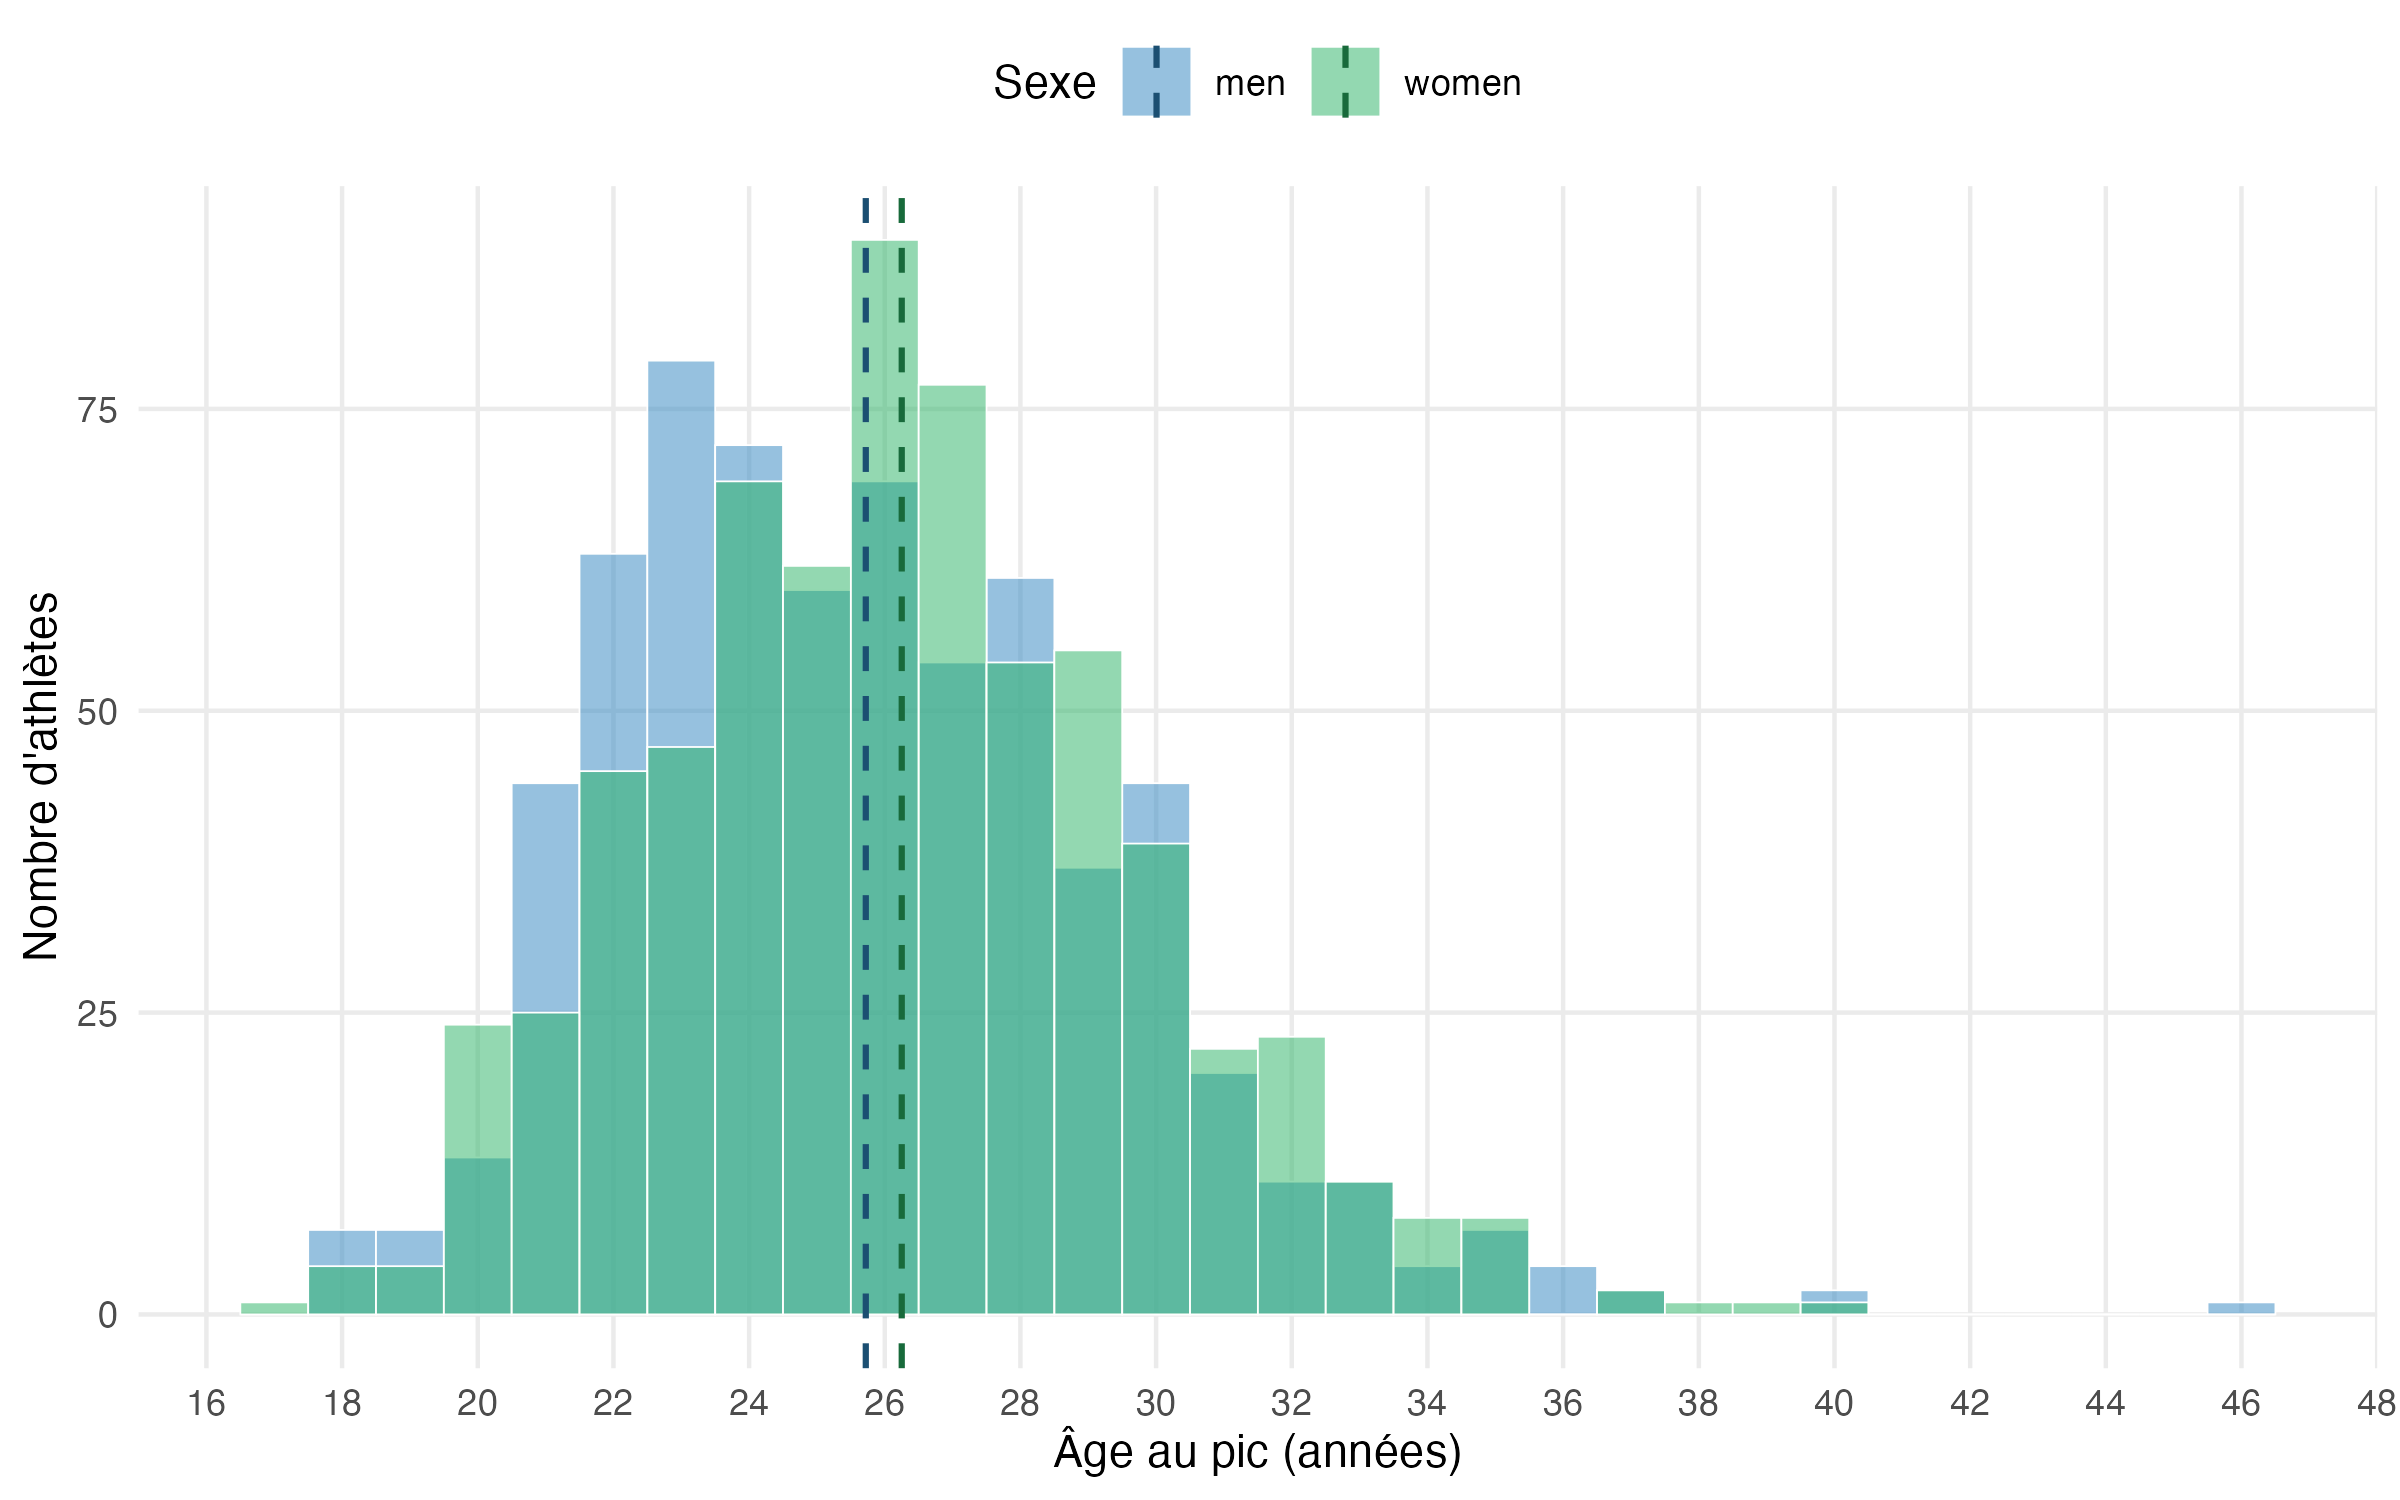
\includegraphics[width=0.85\textwidth]{outputs/histogramme_global.png}}

}

\caption{\label{fig-hist}Distribution de l'âge au pic}

\end{figure}%

Les indicateurs de position associés à cette distribution sont détaillés
dans le tableau ci-dessous :

\begin{longtable}[]{@{}lccccccc@{}}
\caption{Résumé statistique de l'âge au pic observé selon le
sexe}\label{tbl-stats}\tabularnewline
\toprule\noalign{}
Sexe & Eff. & Min & Q1 & Moyenne \(\pm\) SD & Médiane & Q3 & Max \\
\midrule\noalign{}
\endfirsthead
\toprule\noalign{}
Sexe & Eff. & Min & Q1 & Moyenne \(\pm\) SD & Médiane & Q3 & Max \\
\midrule\noalign{}
\endhead
\bottomrule\noalign{}
\endlastfoot
Hommes & 672 & 18 & 23 & 25.72 \(\pm\) 3.74 & \textbf{25} & 28 & 46 \\
Femmes & 672 & 17 & 24 & 26.25 \(\pm\) 3.60 & \textbf{26} & 29 & 40 \\
\end{longtable}

Une différence d'un an est observée sur l'âge médian, s'établissant à 25
ans chez les hommes contre 26 ans chez les femmes. La répartition par
familles de disciplines (Figure~\ref{fig-box}) montre également des
variations de maturité sensibles selon les spécialités.

\begin{figure}

\centering{

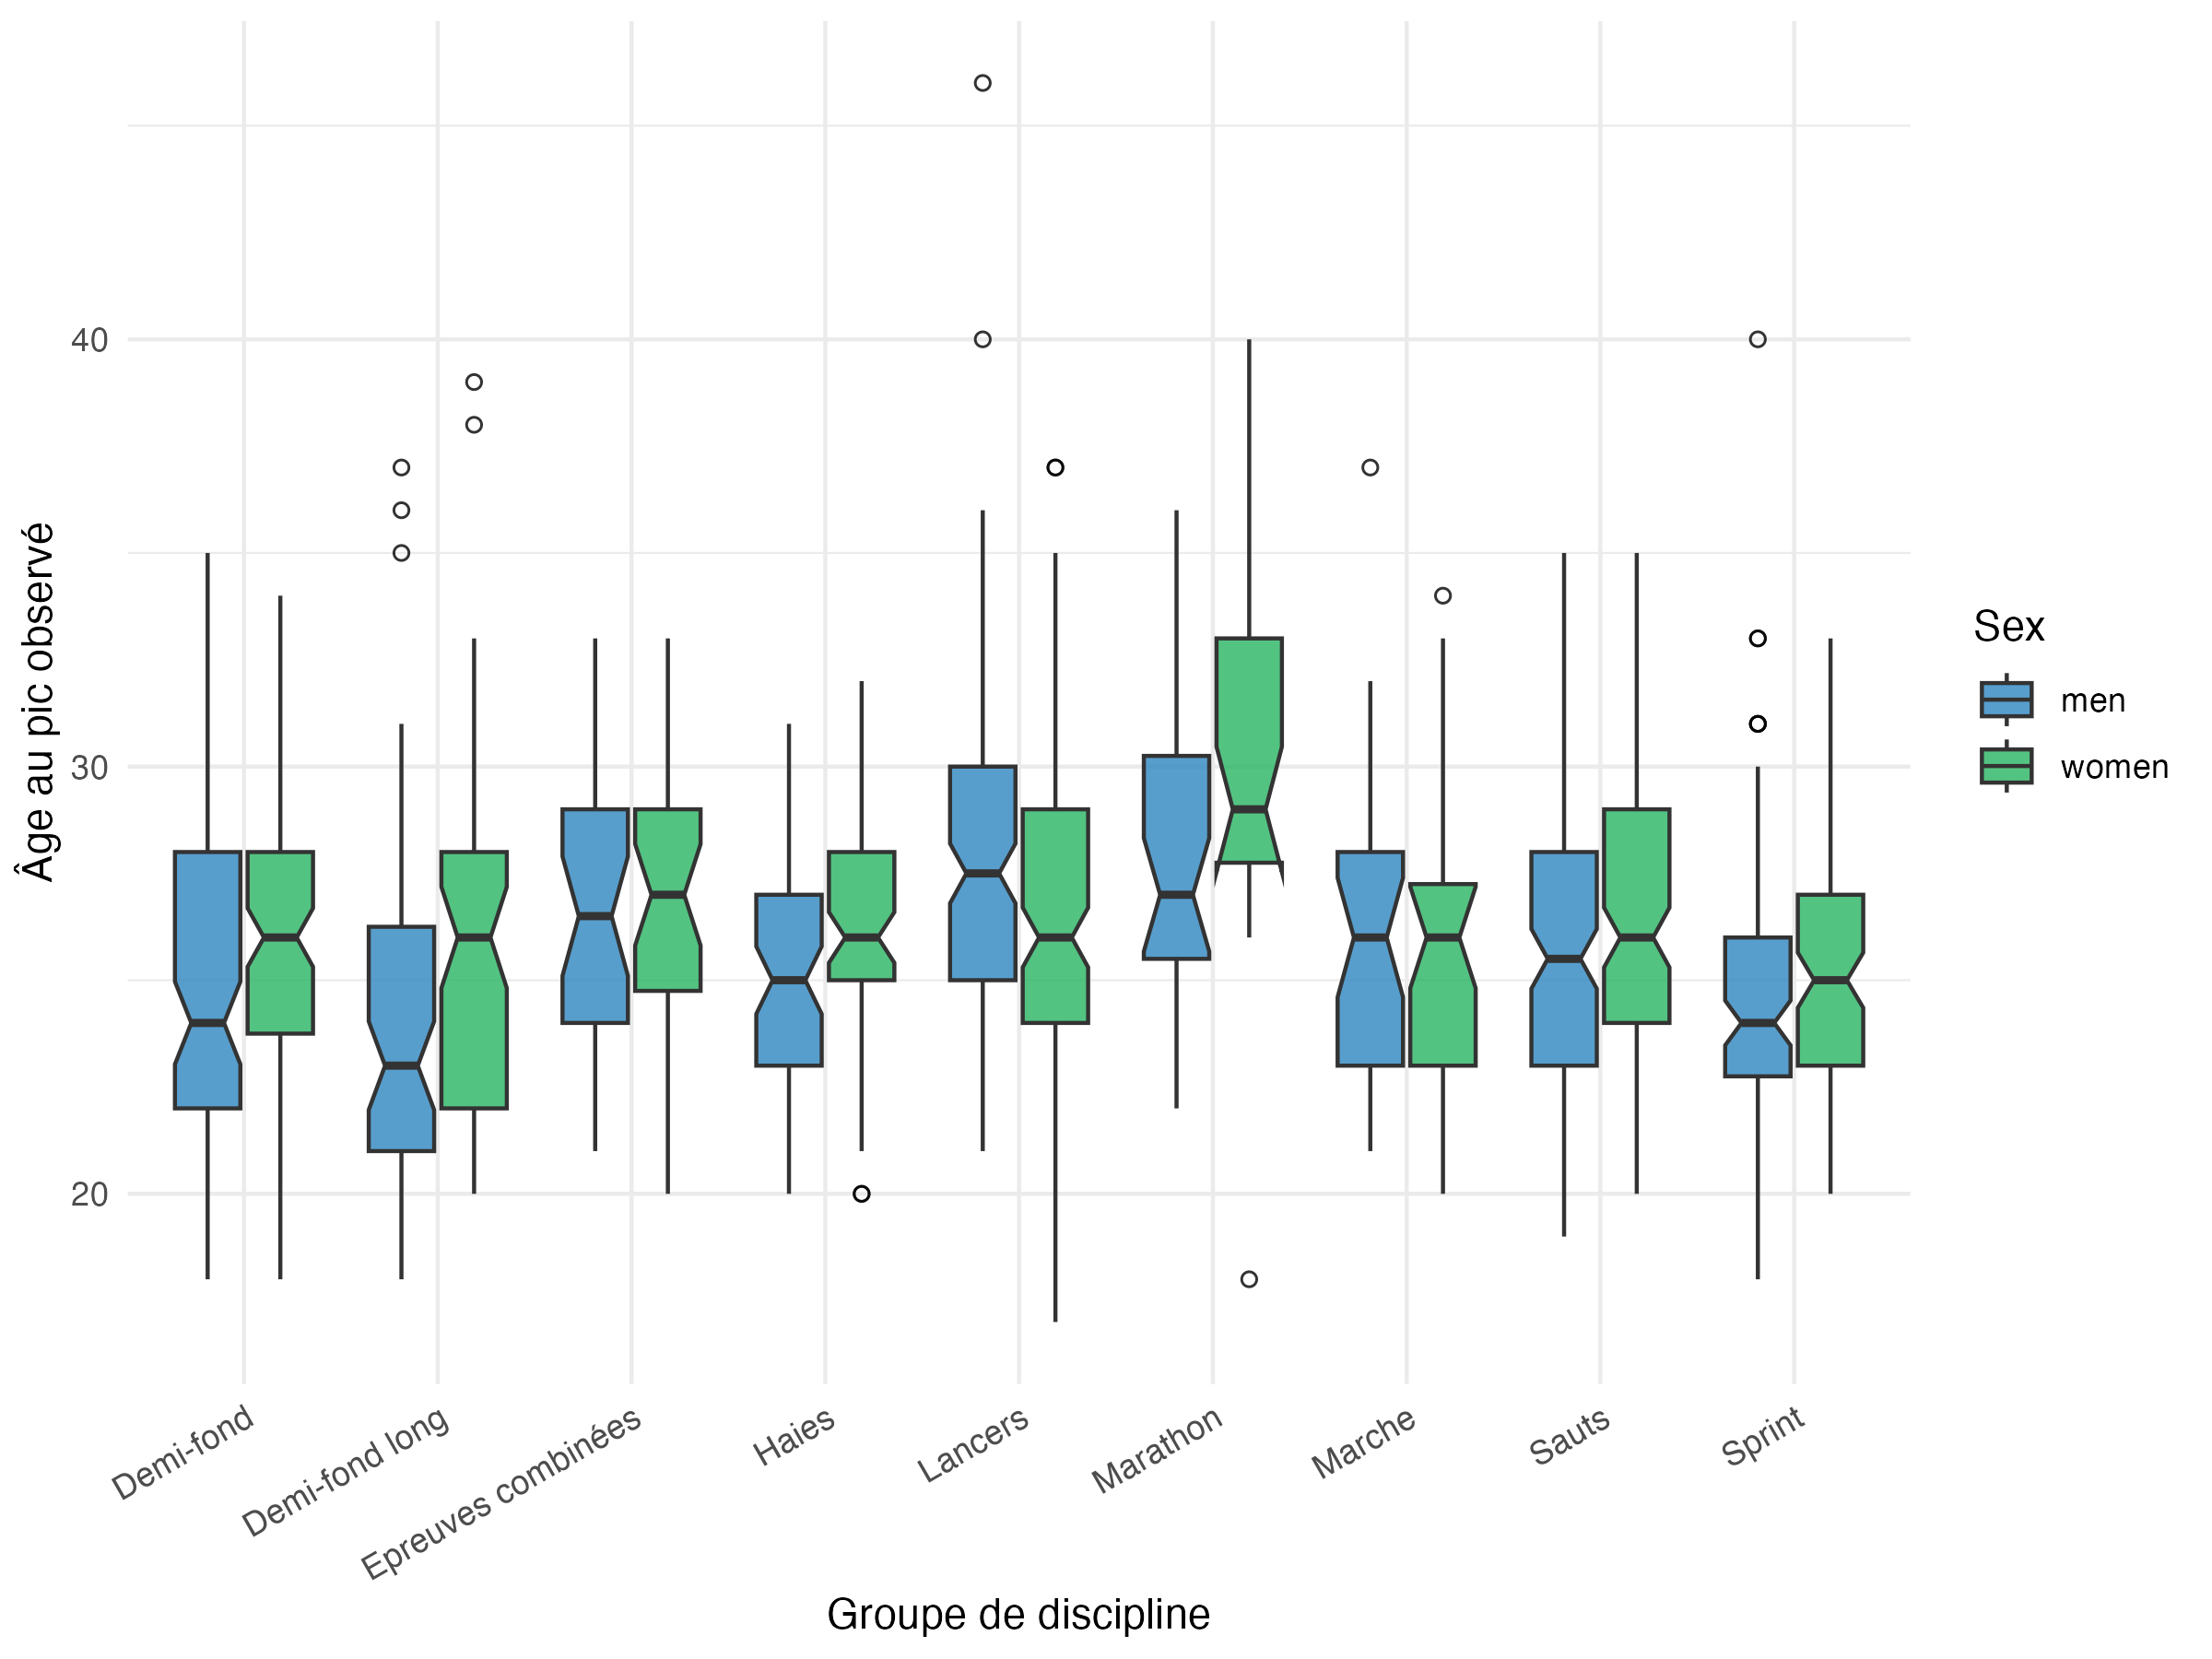
\includegraphics[width=0.85\linewidth,height=\textheight,keepaspectratio]{outputs/boxplot_familles.png}

}

\caption{\label{fig-box}Âges au pic observés selon les familles de
disciplines et le sexe}

\end{figure}%

Le groupe \textbf{Sprint} est identifié comme le plus précoce (médianes
basses). À l'inverse, les \textbf{Lancers} et les disciplines de fond
affichent une maturité plus tardive.

\subsection*{Étude de la distribution et vérification de la
normalité}\label{uxe9tude-de-la-distribution-et-vuxe9rification-de-la-normalituxe9}
\addcontentsline{toc}{subsection}{Étude de la distribution et
vérification de la normalité}

Avant de procéder aux tests d'inférence, il est indispensable d'étudier
la forme de la distribution de notre variable d'intérêt : l'âge au pic
observé. Cette étape permet de vérifier si les données suivent une loi
normale, condition \emph{sine qua non} pour l'utilisation de tests
paramétriques classiques.

\subsubsection*{Analyse visuelle par les
histogrammes}\label{analyse-visuelle-par-les-histogrammes}
\addcontentsline{toc}{subsubsection}{Analyse visuelle par les
histogrammes}

L'examen des histogrammes permet d'observer la répartition réelle des
athlètes par classe d'âge. La Figure~\ref{fig-hist-men} présente cette
distribution pour les athlètes masculins, segmentée par Famille de
disciplines.

\begin{figure}

\centering{

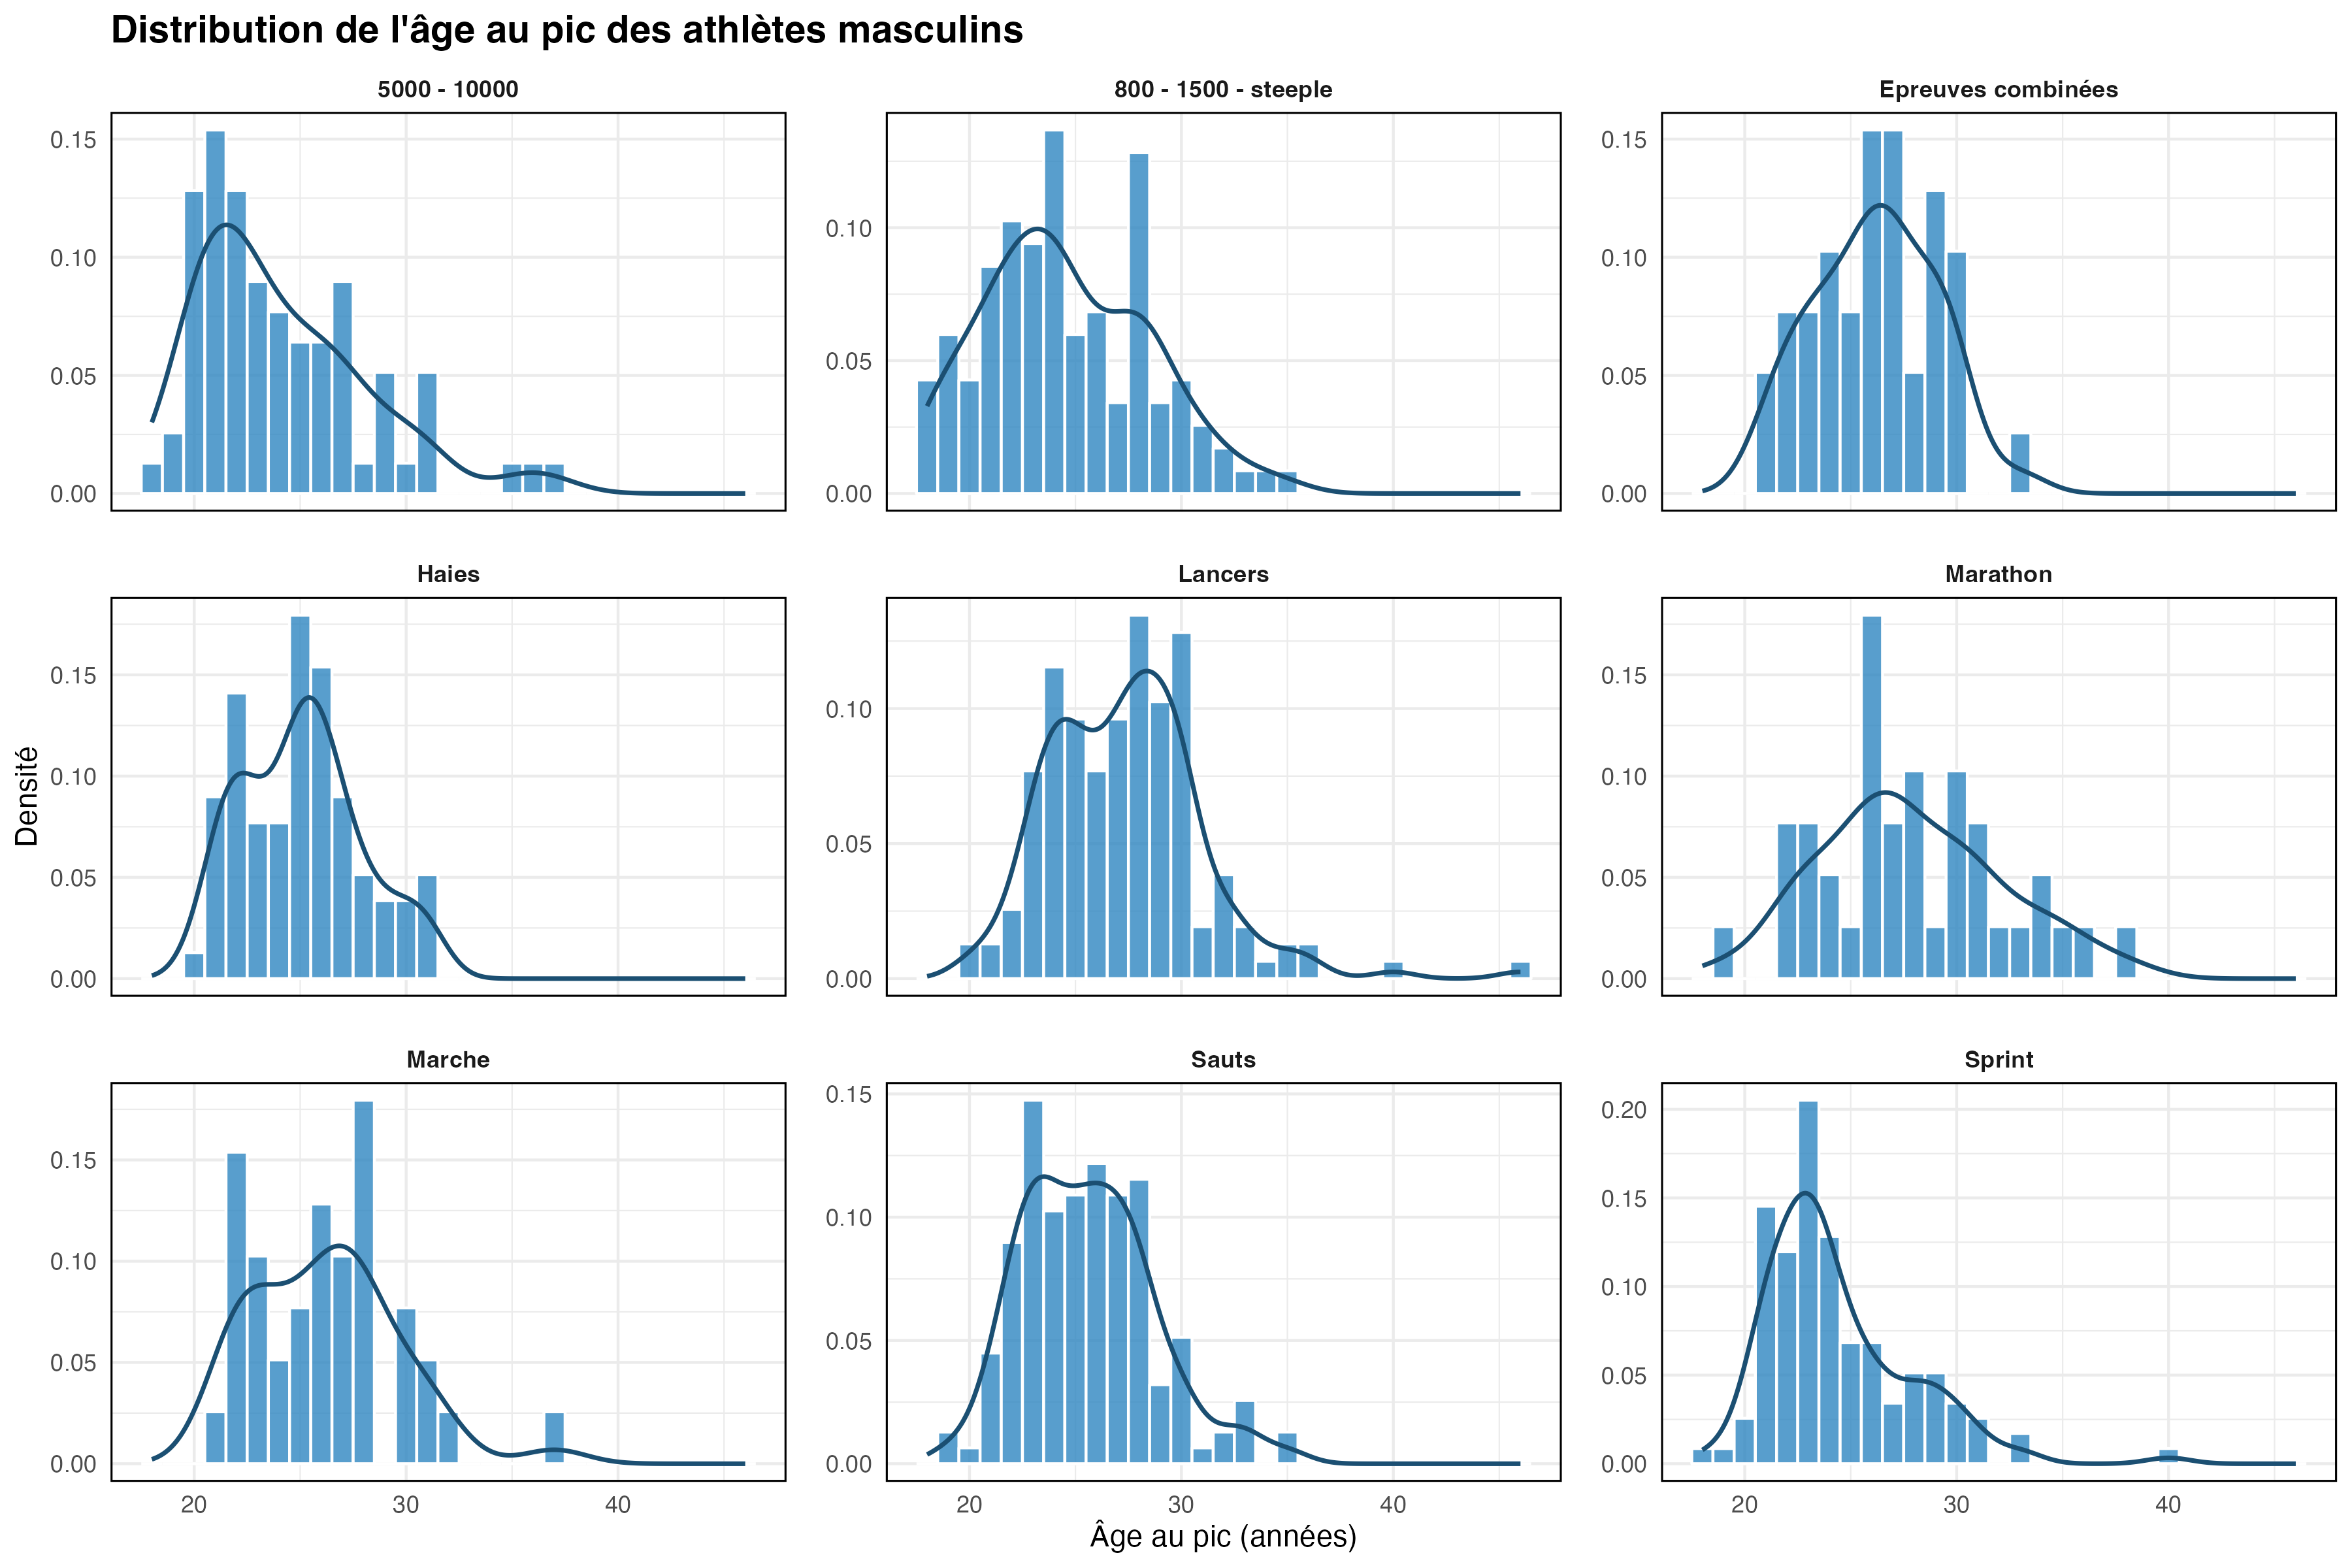
\includegraphics[width=1\linewidth,height=\textheight,keepaspectratio]{outputs/hist_age_hommes.png}

}

\caption{\label{fig-hist-men}Distributions de l'âge au pic de
performance (Athlètes masculins)}

\end{figure}%

L'observation de la Figure~\ref{fig-hist-men} révèle des profils variés
:

\begin{itemize}
\tightlist
\item
  Certaines familles, comme le \textbf{Sprint}, montrent une
  concentration très marquée sur des âges précoces avec une chute rapide
  de l'effectif.
\item
  D'autres, comme les \textbf{Lancers}, présentent une distribution plus
  étalée, suggérant une plus grande hétérogénéité des âges de
  performance.
\item
  De manière générale, on observe une ``queue'' de distribution vers la
  droite (asymétrie positive), indiquant que si l'accès au haut niveau
  est limité avant 20 ans, le maintien de la performance peut se
  prolonger tardivement pour certains individus.
\end{itemize}

\emph{Note : Les histogrammes concernant les athlètes féminines ainsi
que l'ensemble des graphiques Quantile-Quantile (QQ-plots) sont
consultables en Annexe.}

\subsubsection*{Test statistique de normalité
(Shapiro-Wilk)}\label{test-statistique-de-normalituxe9-shapiro-wilk}
\addcontentsline{toc}{subsubsection}{Test statistique de normalité
(Shapiro-Wilk)}

Pour confirmer ces observations visuelles, un test de
\textbf{Shapiro-Wilk} a été réalisé sur chaque groupe. Ce test évalue
l'hypothèse nulle (\(H_0\)) de normalité des données. Si la \(p\)-value
est inférieure au seuil de \(5\%\), l'hypothèse de normalité est
rejetée.

\begin{longtable}[]{@{}lcccc@{}}
\caption{Résultats du test de normalité de Shapiro-Wilk par
groupe}\label{tbl-shapiro}\tabularnewline
\toprule\noalign{}
Famille & Sexe & Statistique W & \(p\)-value & Normalité \\
\midrule\noalign{}
\endfirsthead
\toprule\noalign{}
Famille & Sexe & Statistique W & \(p\)-value & Normalité \\
\midrule\noalign{}
\endhead
\bottomrule\noalign{}
\endlastfoot
5000 - 10000 & Hommes & 0.883 & \textless{} 0.001 & \textbf{NON} \\
5000 - 10000 & Femmes & 0.943 & 0.005 & \textbf{NON} \\
800 - 1500 - steeple & Hommes & 0.969 & 0.023 & \textbf{NON} \\
Sprint & Hommes & 0.892 & \textless{} 0.001 & \textbf{NON} \\
Lancers & Hommes & 0.915 & \textless{} 0.001 & \textbf{NON} \\
Épreuves combinées & Hommes & 0.963 & 0.335 & \textbf{OUI} \\
Marche & Femmes & 0.942 & 0.083 & \textbf{OUI} \\
\end{longtable}

\subsubsection*{Conclusion sur le choix des
tests}\label{conclusion-sur-le-choix-des-tests}
\addcontentsline{toc}{subsubsection}{Conclusion sur le choix des tests}

Les résultats du test de Shapiro-Wilk (Table~\ref{tbl-shapiro})
confirment que la normalité est rejetée pour la majorité des familles
les plus représentées (Sprint, Lancers, Demi-fond). Les quelques cas où
la normalité est acceptée (Épreuves combinées, Marche) correspondent
souvent à des effectifs plus réduits ou à des disciplines aux
contraintes de maturité spécifiques.

\textbf{Implication méthodologique :} La distribution de l'âge au pic
n'étant pas uniformément normale, l'utilisation de la moyenne et de
l'écart-type comme seuls indicateurs serait trompeuse. Par conséquent :
1. La \textbf{médiane} et les \textbf{quartiles} sont privilégiés pour
décrire les positions. 2. Des \textbf{tests non-paramétriques}
(Wilcoxon-Mann-Whitney pour le sexe et Kruskal-Wallis pour les familles)
sont exclusivement utilisés pour comparer les groupes. Ces tests, fondés
sur les rangs, sont robustes face à l'asymétrie et aux valeurs extrêmes
observées.

\subsection*{Discussion}\label{discussion}
\addcontentsline{toc}{subsection}{Discussion}

L'analyse montre que l'âge au pic est une variable plastique, influencée
prioritairement par la filière énergétique sollicitée. Il est possible
que la précocité en sprint soit liée aux exigences de puissance
neuromusculaire, tandis que la maturité tardive dans les lancers ou le
marathon suggère que la force, la technique ou l'efficience aérobie
peuvent se bonifier avec l'expérience.

Il est important de noter que si des tendances générales existent, les
performances exceptionnelles liées à des individus uniques (comme le
record de longévité à 46 ans identifié dans l'échantillon) ne peuvent
être généralisées. Cette hétérogénéité valide la stratégie consistant à
calibrer les modèles de Moore et IMAP de façon spécifique pour chaque
sous-groupe afin de capturer la tendance moyenne de la population
d'élite.

\newpage

\subsubsection{Description des tests statistiques
utilisés}\label{description-des-tests-statistiques-utilisuxe9s}

Trois tests principaux ont été mobilisés pour valider les observations
descriptives :

\begin{itemize}
\tightlist
\item
  \textbf{Test de Wilcoxon-Mann-Whitney :} Utilisé pour comparer l'âge
  au pic entre les deux sexes (deux groupes indépendants). Contrairement
  au test \(t\) de Student, il ne compare pas les moyennes mais teste si
  une distribution est statistiquement décalée par rapport à l'autre en
  se basant sur la somme des rangs.
\item
  \textbf{Test de Kruskal-Wallis :} Appliqué pour comparer l'âge au pic
  entre les différentes familles de disciplines (plus de deux groupes
  indépendants). Il constitue l'alternative non paramétrique à l'ANOVA à
  un facteur. L'hypothèse nulle (\(H_0\)) suppose que les médianes de
  tous les groupes sont identiques.
\item
  \textbf{Test post-hoc de Dunn :} Lorsqu'une différence significative a
  été détectée par le test de Kruskal-Wallis, le test de Dunn a été
  utilisé pour effectuer des comparaisons par paires entre les familles
  (ex: Sprint vs Lancers). Une correction de \textbf{Bonferroni} a été
  systématiquement appliquée aux p-values pour limiter le risque
  d'erreur de type I (faux positifs) lié à la multiplicité des tests.
\end{itemize}

L'ensemble des calculs a été effectué avec un seuil de significativité
\(\alpha = 0.05\).

\subsection{Résultats}\label{ruxe9sultats}

L'examen de la distribution globale (Figure 1) montre que la majorité
des athlètes atteignent leur record personnel dans une fenêtre comprise
entre 22 et 28 ans.

\begin{figure}

\centering{

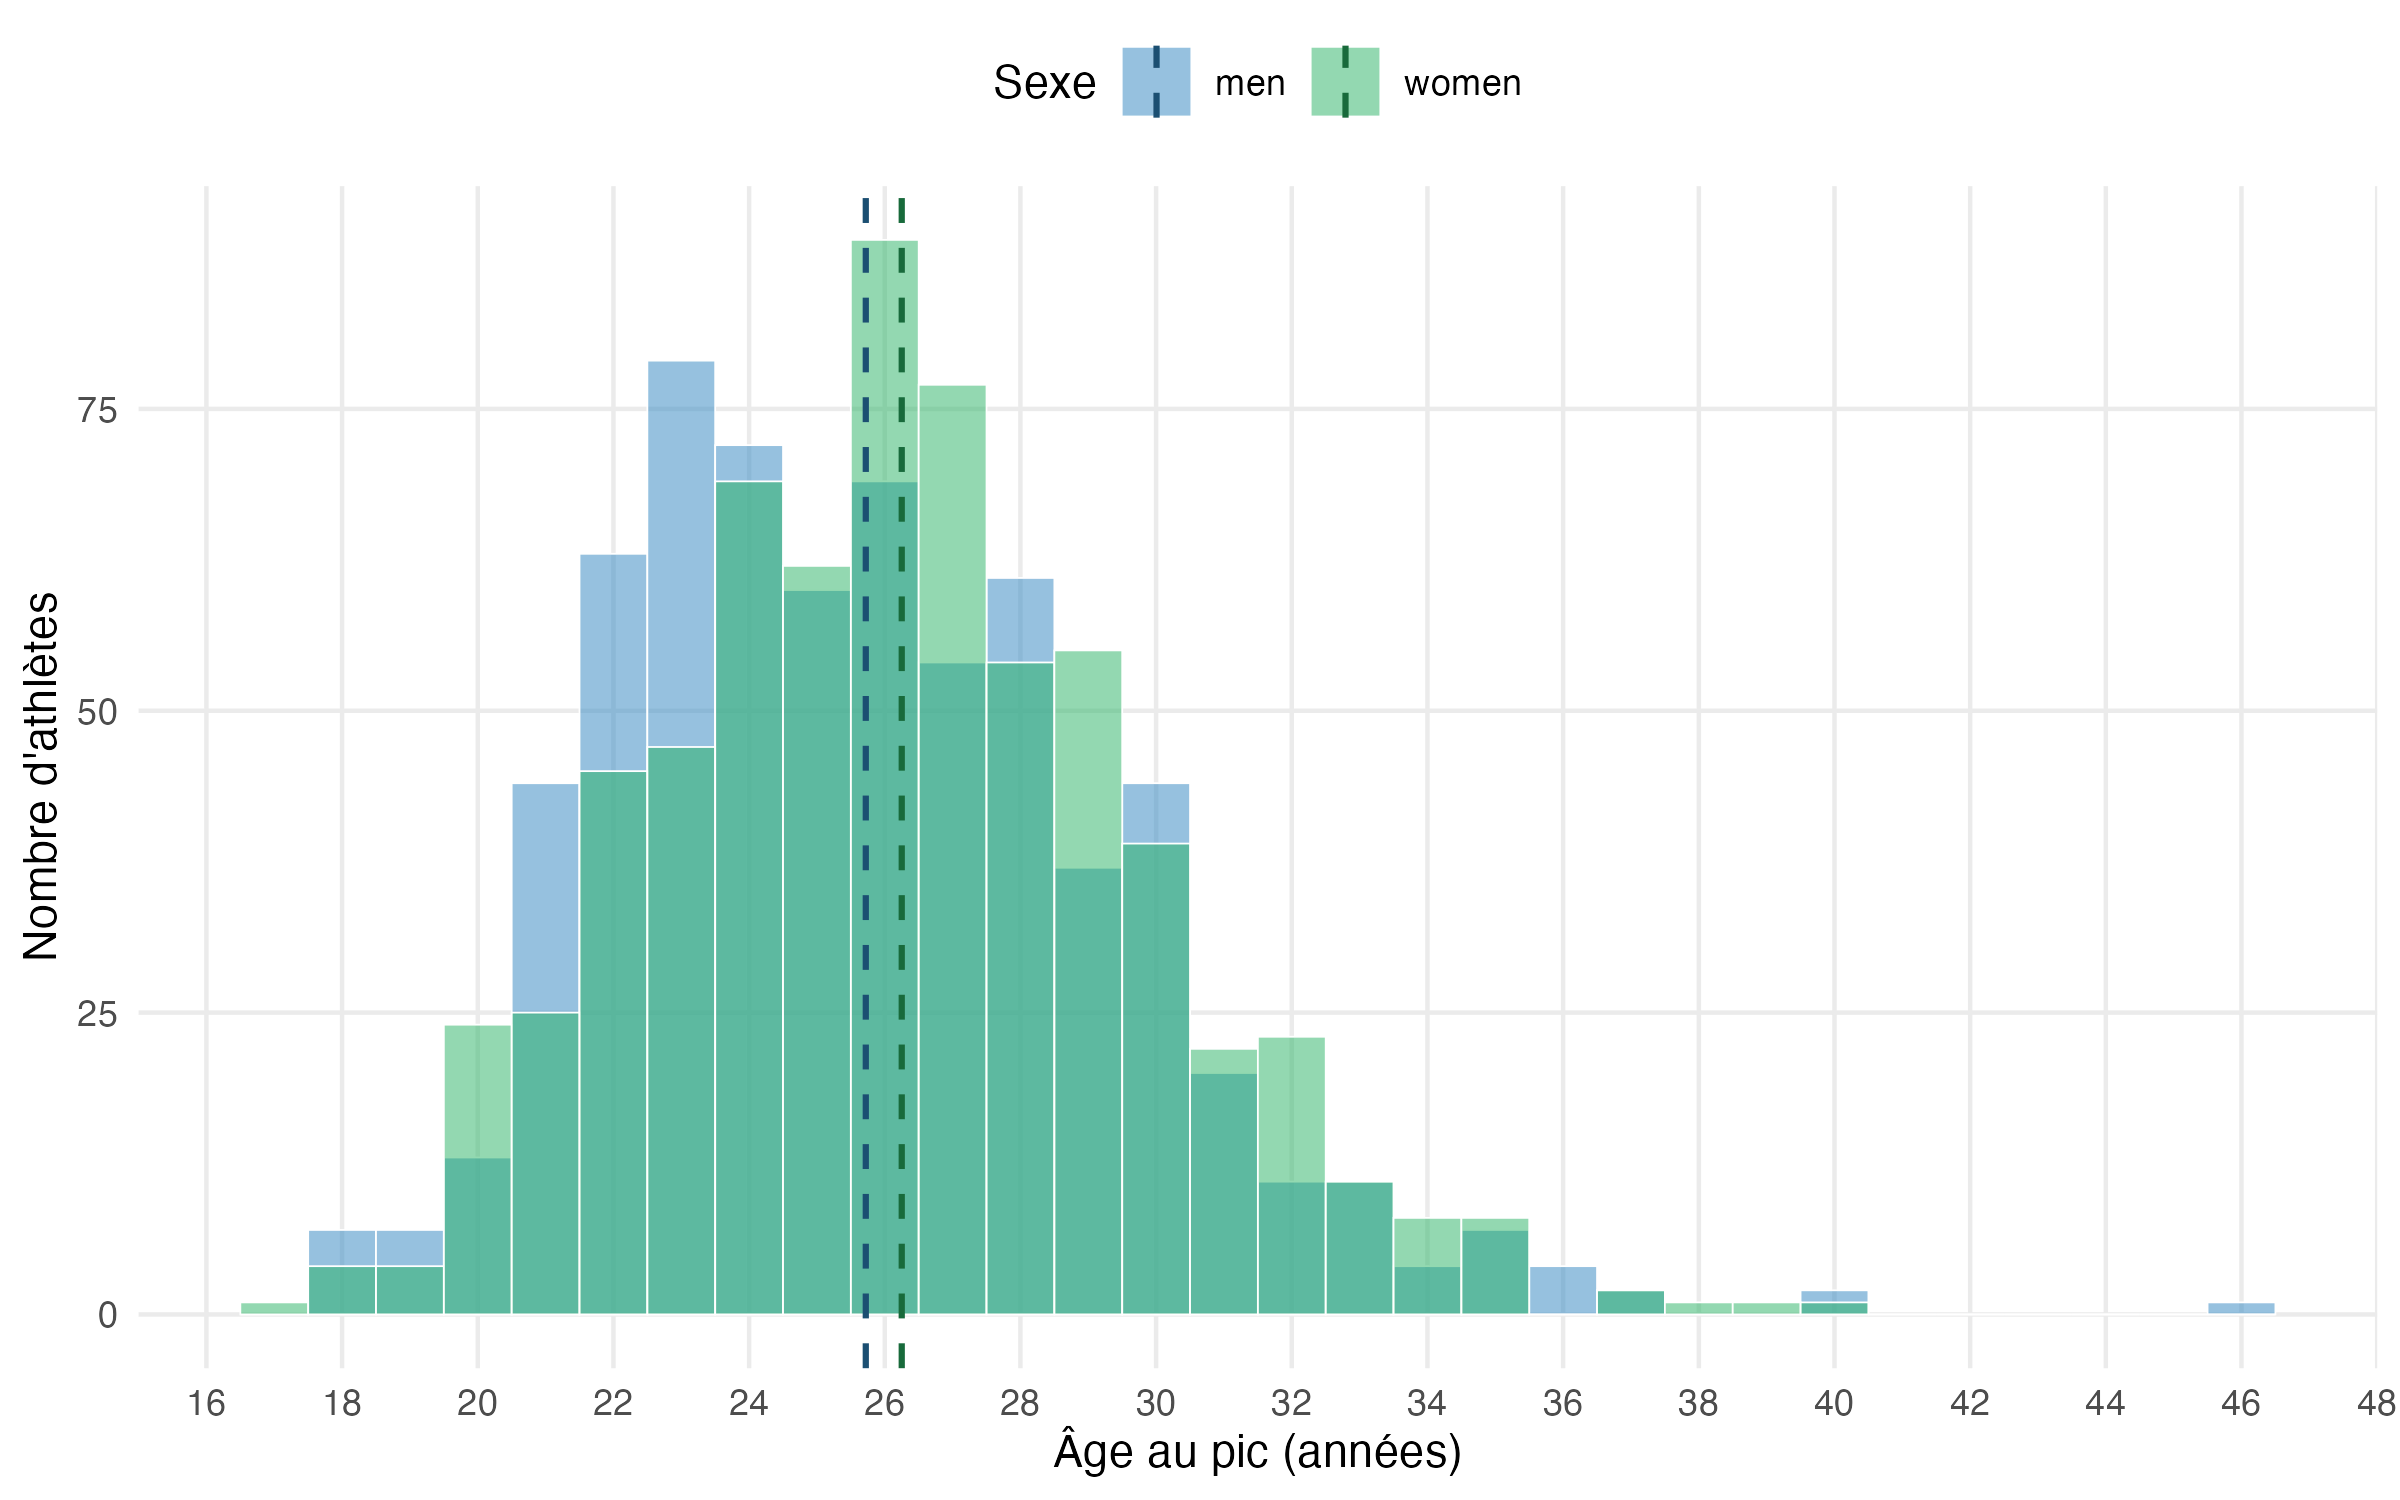
\includegraphics[width=0.85\linewidth,height=\textheight,keepaspectratio]{outputs/histogramme_global.png}

}

\caption{\label{fig-hist}Distribution de l'âge au pic de performance
selon le sexe}

\end{figure}%

Une différence est observée dans la répartition : la distribution
masculine semble plus dense dans la zone de précocité (21-23 ans),
tandis que la distribution féminine présente un sommet plus marqué
autour de 26 ans. Le Tableau 1 détaille ces indicateurs de position.

\begin{longtable}[]{@{}lccccccc@{}}
\caption{Résumé statistique de l'âge au pic observé selon le
sexe}\label{tbl-stats}\tabularnewline
\toprule\noalign{}
Sexe & Eff. & Min & Q1 & Moyenne \(\pm\) SD & Médiane & Q3 & Max \\
\midrule\noalign{}
\endfirsthead
\toprule\noalign{}
Sexe & Eff. & Min & Q1 & Moyenne \(\pm\) SD & Médiane & Q3 & Max \\
\midrule\noalign{}
\endhead
\bottomrule\noalign{}
\endlastfoot
Hommes & 507 & 18 & 23 & 25.56 \(\pm\) 4.06 & 25 & 28 & 46 \\
Femmes & 507 & 17 & 24 & 26.17 \(\pm\) 3.80 & 26 & 29 & 40 \\
\end{longtable}

D'après ces données, l'âge médian au pic est d'un an supérieur chez les
femmes (26 ans) par rapport aux hommes (25 ans). Le résultat du test de
Wilcoxon-Mann-Whitney (\(p = 0.004\)) permet de rejeter l'hypothèse
nulle : il existe une différence statistiquement significative dans le
timing de la performance entre les deux groupes.

\subsubsection{Analyse par familles de
disciplines}\label{analyse-par-familles-de-disciplines}

Le boxplot de la Figure 2 permet de visualiser les différences d'âge au
pic entre les groupes de disciplines et entre les sexes. On observe
d'abord que ces données varient sensiblement d'un groupe de disciplines
à l'autre.

\begin{figure}

\centering{

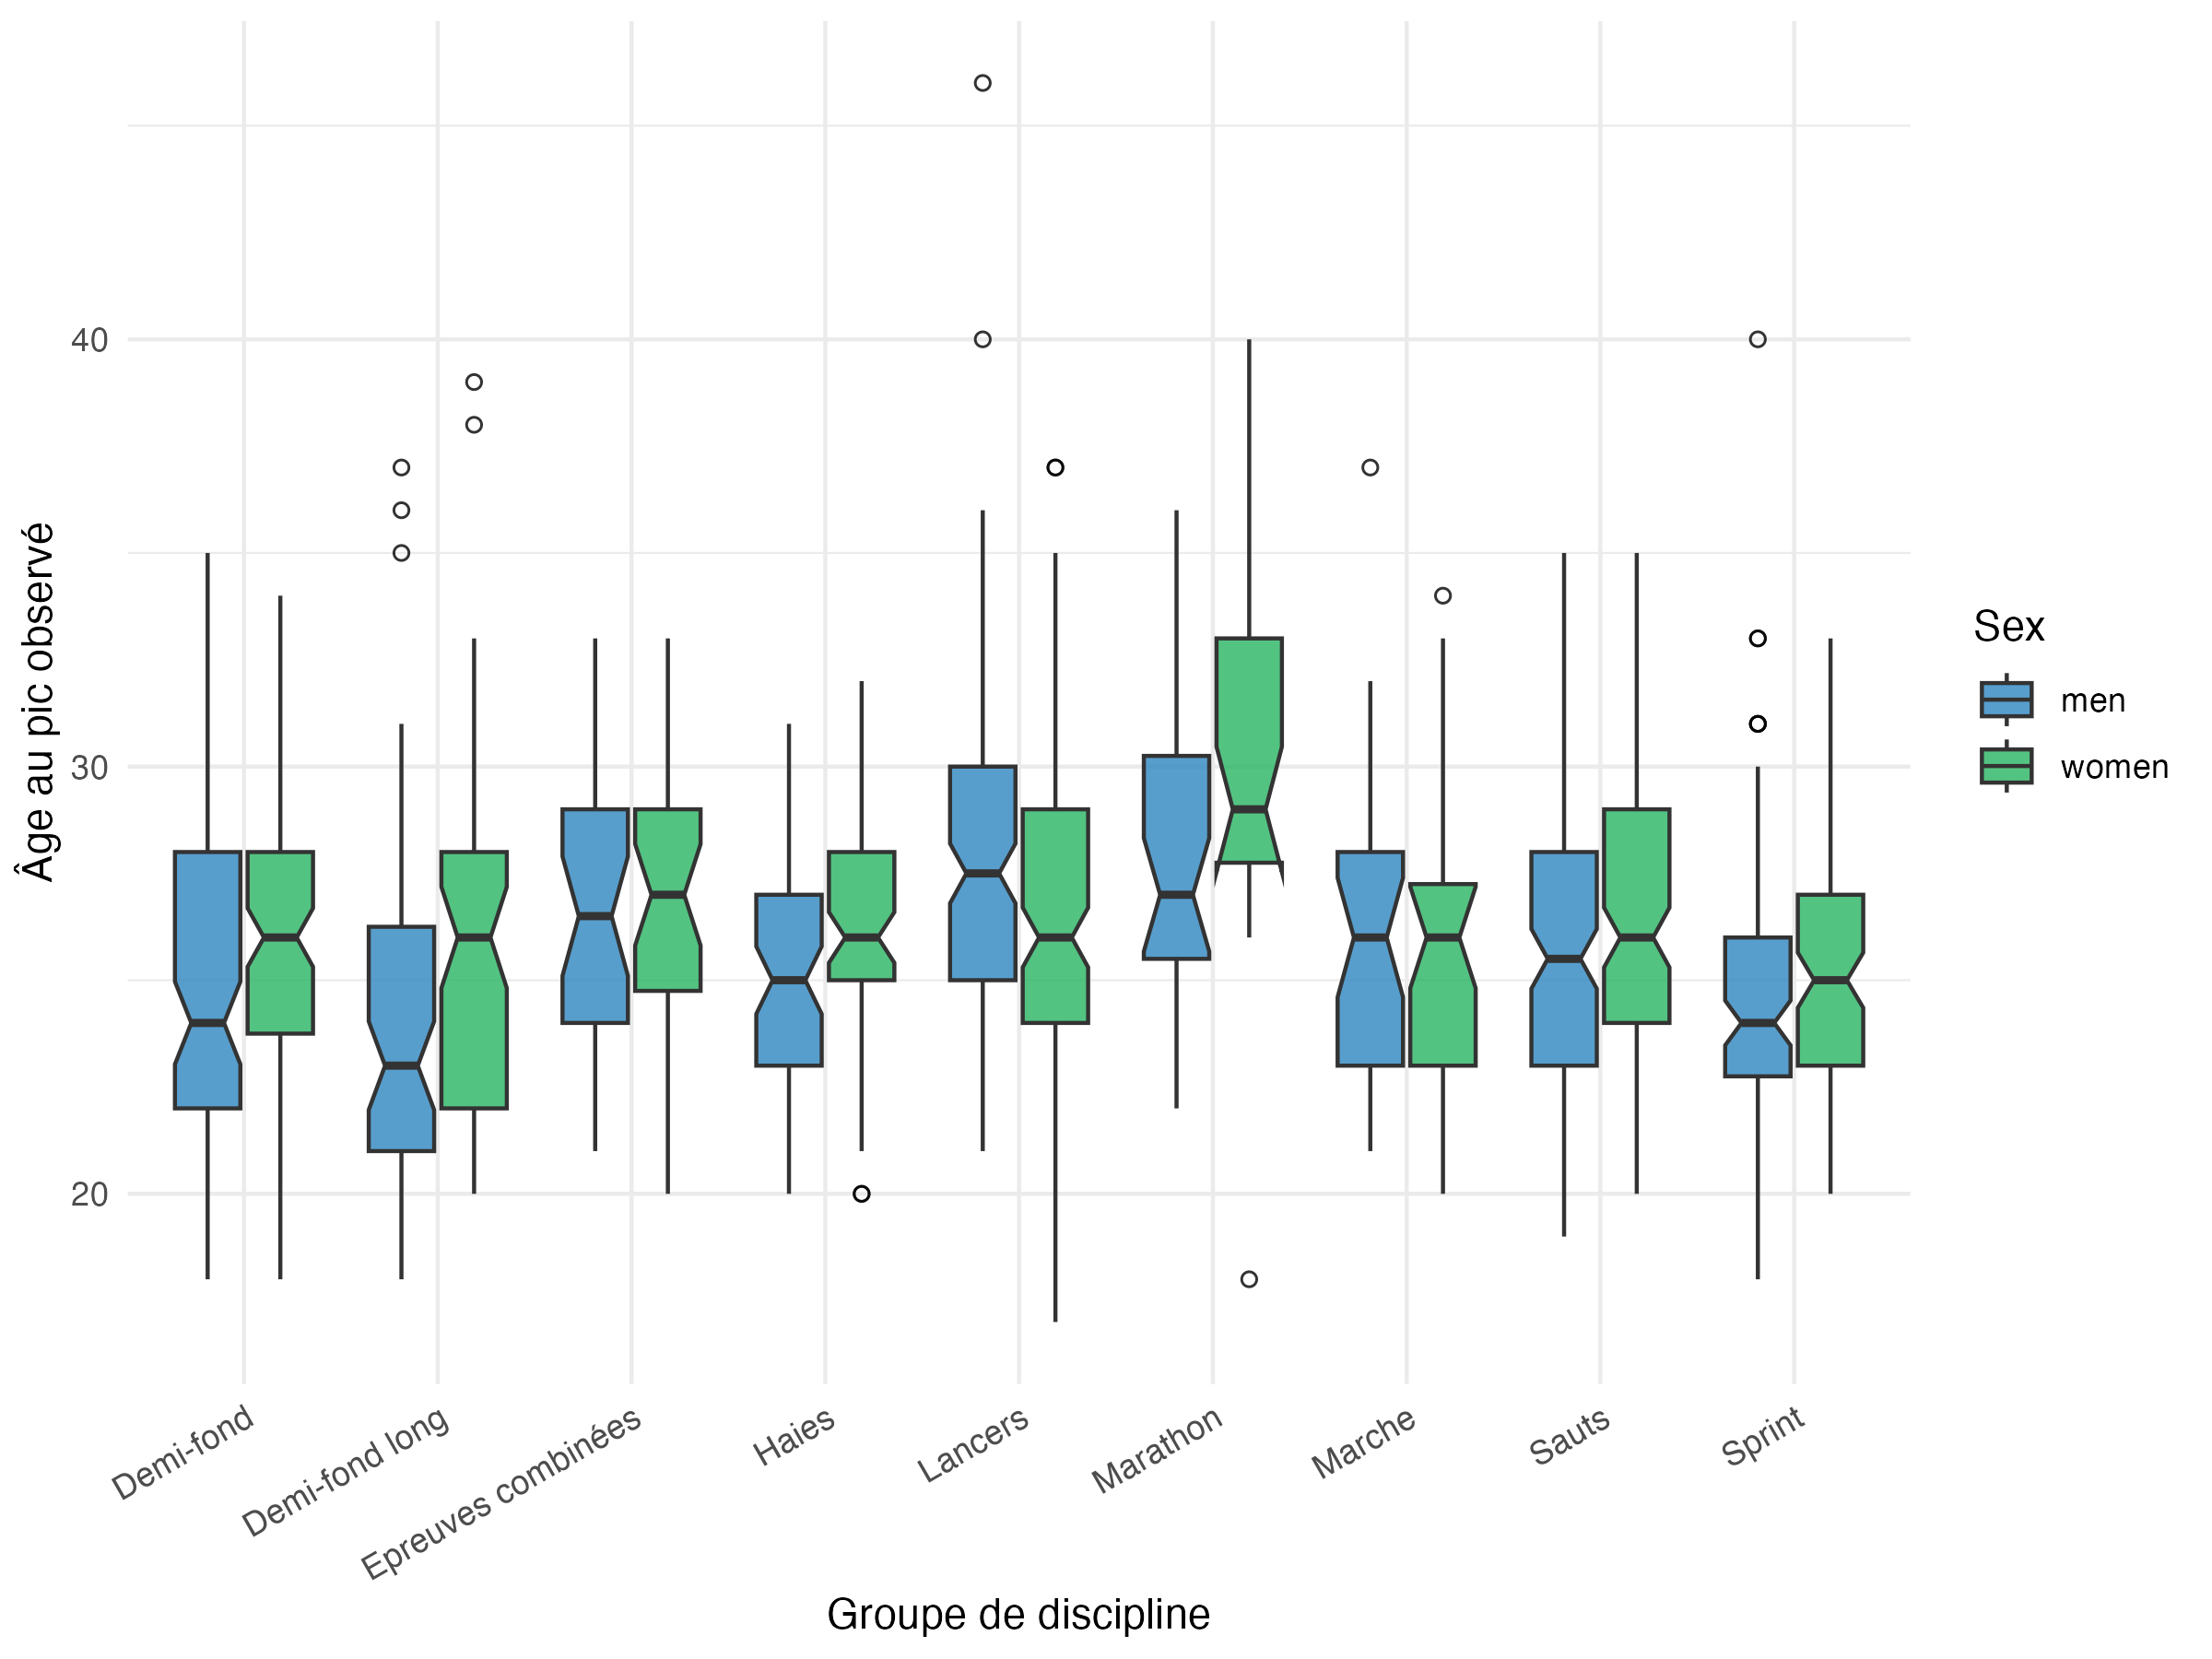
\includegraphics[width=0.85\linewidth,height=\textheight,keepaspectratio]{outputs/boxplot_familles.png}

}

\caption{\label{fig-box}Âges au pic observés selon les familles de
disciplines et le sexe}

\end{figure}%

Le groupe \textbf{Sprint} est identifié comme le plus précoce (médiane à
23-24 ans). À l'inverse, les \textbf{Lancers} et les disciplines
d'\textbf{Endurance longue} affichent une maturité plus tardive. Le test
de Kruskal-Wallis confirme la solidité de ces écarts
(\(\chi^2 = 38.855, p < 0.001\)). Les comparaisons par paires via le
test de Dunn soulignent que le groupe Sprint diffère significativement
des Lancers (\(p < 0.001\)) et de l'Endurance (\(p = 0.002\)).

\subsection{Discussion}\label{discussion-1}

L'analyse montre que l'âge au pic est une variable plastique, influencée
prioritairement par la filière énergétique sollicitée. La précocité en
sprint pourrait être liée aux exigences de puissance neuromusculaire,
tandis que la maturité tardive dans les lancers ou le marathon suggère
que la force, la technique ou l'efficience aérobie peuvent se bonifier
avec l'expérience.

Il est important de noter que si des tendances générales existent, les
performances exceptionnelles liées à des individus uniques (comme le
record de longévité à 46 ans identifié dans l'échantillon) ne peuvent
être généralisées. Cette hétérogénéité valide la stratégie consistant à
calibrer les modèles de Moore et IMAP de façon spécifique pour chaque
sous-groupe afin de capturer la tendance moyenne de la population
d'élite.

\newpage

\section{Etude 2 : Modèles}\label{etude-2-moduxe8les}

\subsection{Méthodologie}\label{muxe9thodologie-1}

De nombreux modèles ont déjà été élaborés afin de modéliser la relation
entre l'âge et la performance en athlétisme. Nous allons nous concentrer
sur le modèle de Moore (1975) ainsi que sur le modèle IMAP (2019). Ces
deux modèles sont des modèles incluant une partie qui va croitre avec
l'âge jusqu'à atteindre un pic ainsi qu'une seconde partie de
décroissance.

\subsubsection{Modèle de Moore (1975)}\label{moduxe8le-de-moore-1975}

Dans son modèle, Dan H. Moore explique la relation entre l'âge et la
performance sur un large éventail d'âges, de 5 ans jusqu'à 75 ans. Il
utilise l'équation suivante pour modéliser la performance en fonction de
l'âge.

\begin{equation}\phantomsection\label{eq-moore}{P(t) = a \cdot(1 - e^{-bt}) + c \cdot(1 - e^{dt})}\end{equation}

L'équation \eqref{eq:moore} est un modèle à double exponentielle,
constitué de deux composantes :\\
- \(P_1(t) = a(1 - e^{-bt})\) : correspond à la phase d'amélioration des
performances avec l'âge.\\
- \(P_2(t) = c(1 - e^{dt})\) : correspond à la phase de déclin des
performances, liée au vieillissement.

Dans ce modèle, les paramètres a, b, c et d sont tous positifs et P(t)
correspond à la performance à l'âge t.

En s'appuyant sur l'expression analytique du pic
\(P(t_{pic}) = (a+c) − a·R^{−α} − c·R^{1−α}\) où \(R = \frac {ab} {cd}\)
et \(\alpha = \frac {b} {b+d}\) ainsi que de sa position
\(t_{pic} = \frac {ln(\frac {ab} {cd})} {b+d}\), on peut caractériser
précisément le rôle de chaque paramètre. Les paramètres a et c
gouvernent l'amplitude de la courbe mais agissent en sens opposés : a
détermine le plateau vers lequel tend le terme montant et tire le pic
vers le haut, tandis que c contrôle l'amplitude du terme descendant et
l'abaisse. Leur rapport conditionne ainsi directement la valeur maximale
atteinte par P(t). Sous l'hypothèse c \textless\textless{} a, a est le
paramètre dominant : il fixe à lui seul l'ordre de grandeur du pic, et c
n'en est qu'une correction.

\begin{figure}[H]

{\centering 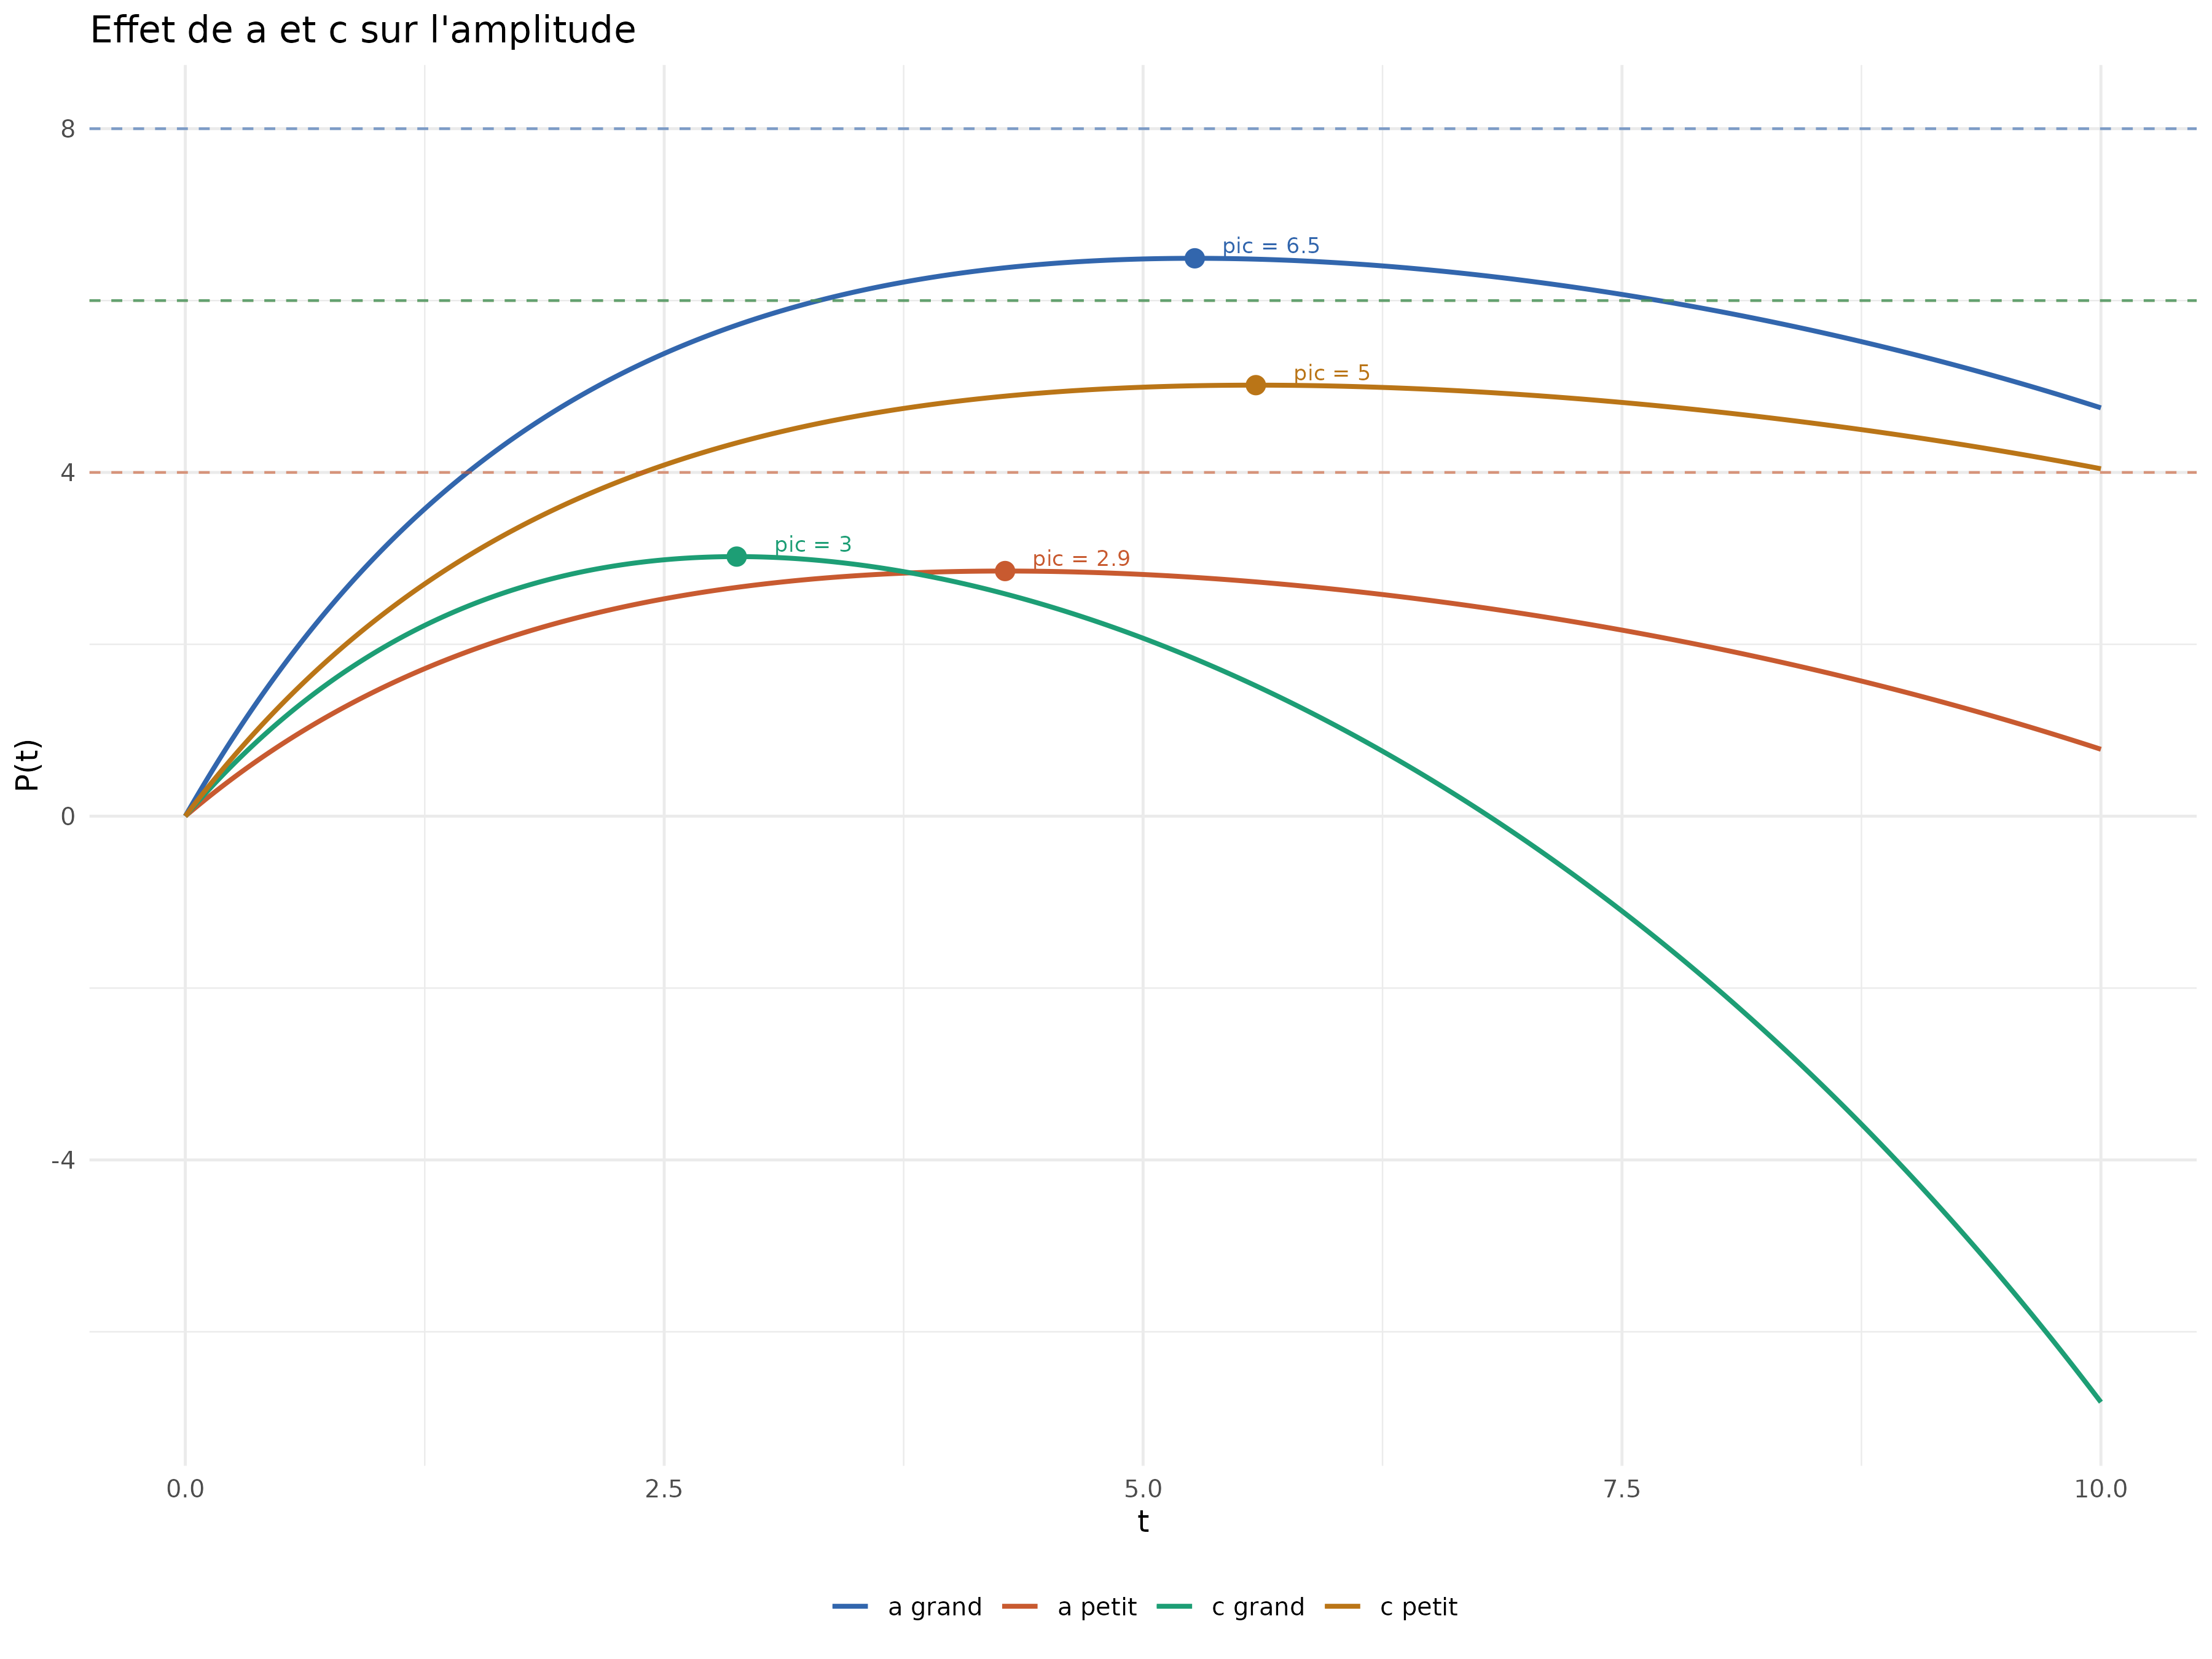
\includegraphics[width=0.8\linewidth,height=\textheight,keepaspectratio]{methodo/a_et_c.png}

}

\caption{Effet de a et c}

\end{figure}%

Les paramètres b et d gouvernent quant à eux la dynamique temporelle de
la courbe. b est la vitesse de montée, il est directement proportionnel
à la pente initiale via P'(0) ≈ ab tandis que d est la vitesse de
descente, estimable depuis la pente de la phase tardive. Leur somme b+d
détermine l'étalement global de la courbe : une grande valeur de b+d
produit un pic étroit et précoce, une petite valeur un pic large et
tardif. La position du pic
\(t_{pic} = \frac {ln(\frac {ab} {cd})} {b+d}\) montre que b et d
interagissent également avec a et c via le rapport
\(R = \frac {ab} {cd}\): le pic est d'autant plus tardif que la force du
terme montant (ab) est grande devant celle du terme descendant (cd).

\begin{figure}[H]

{\centering 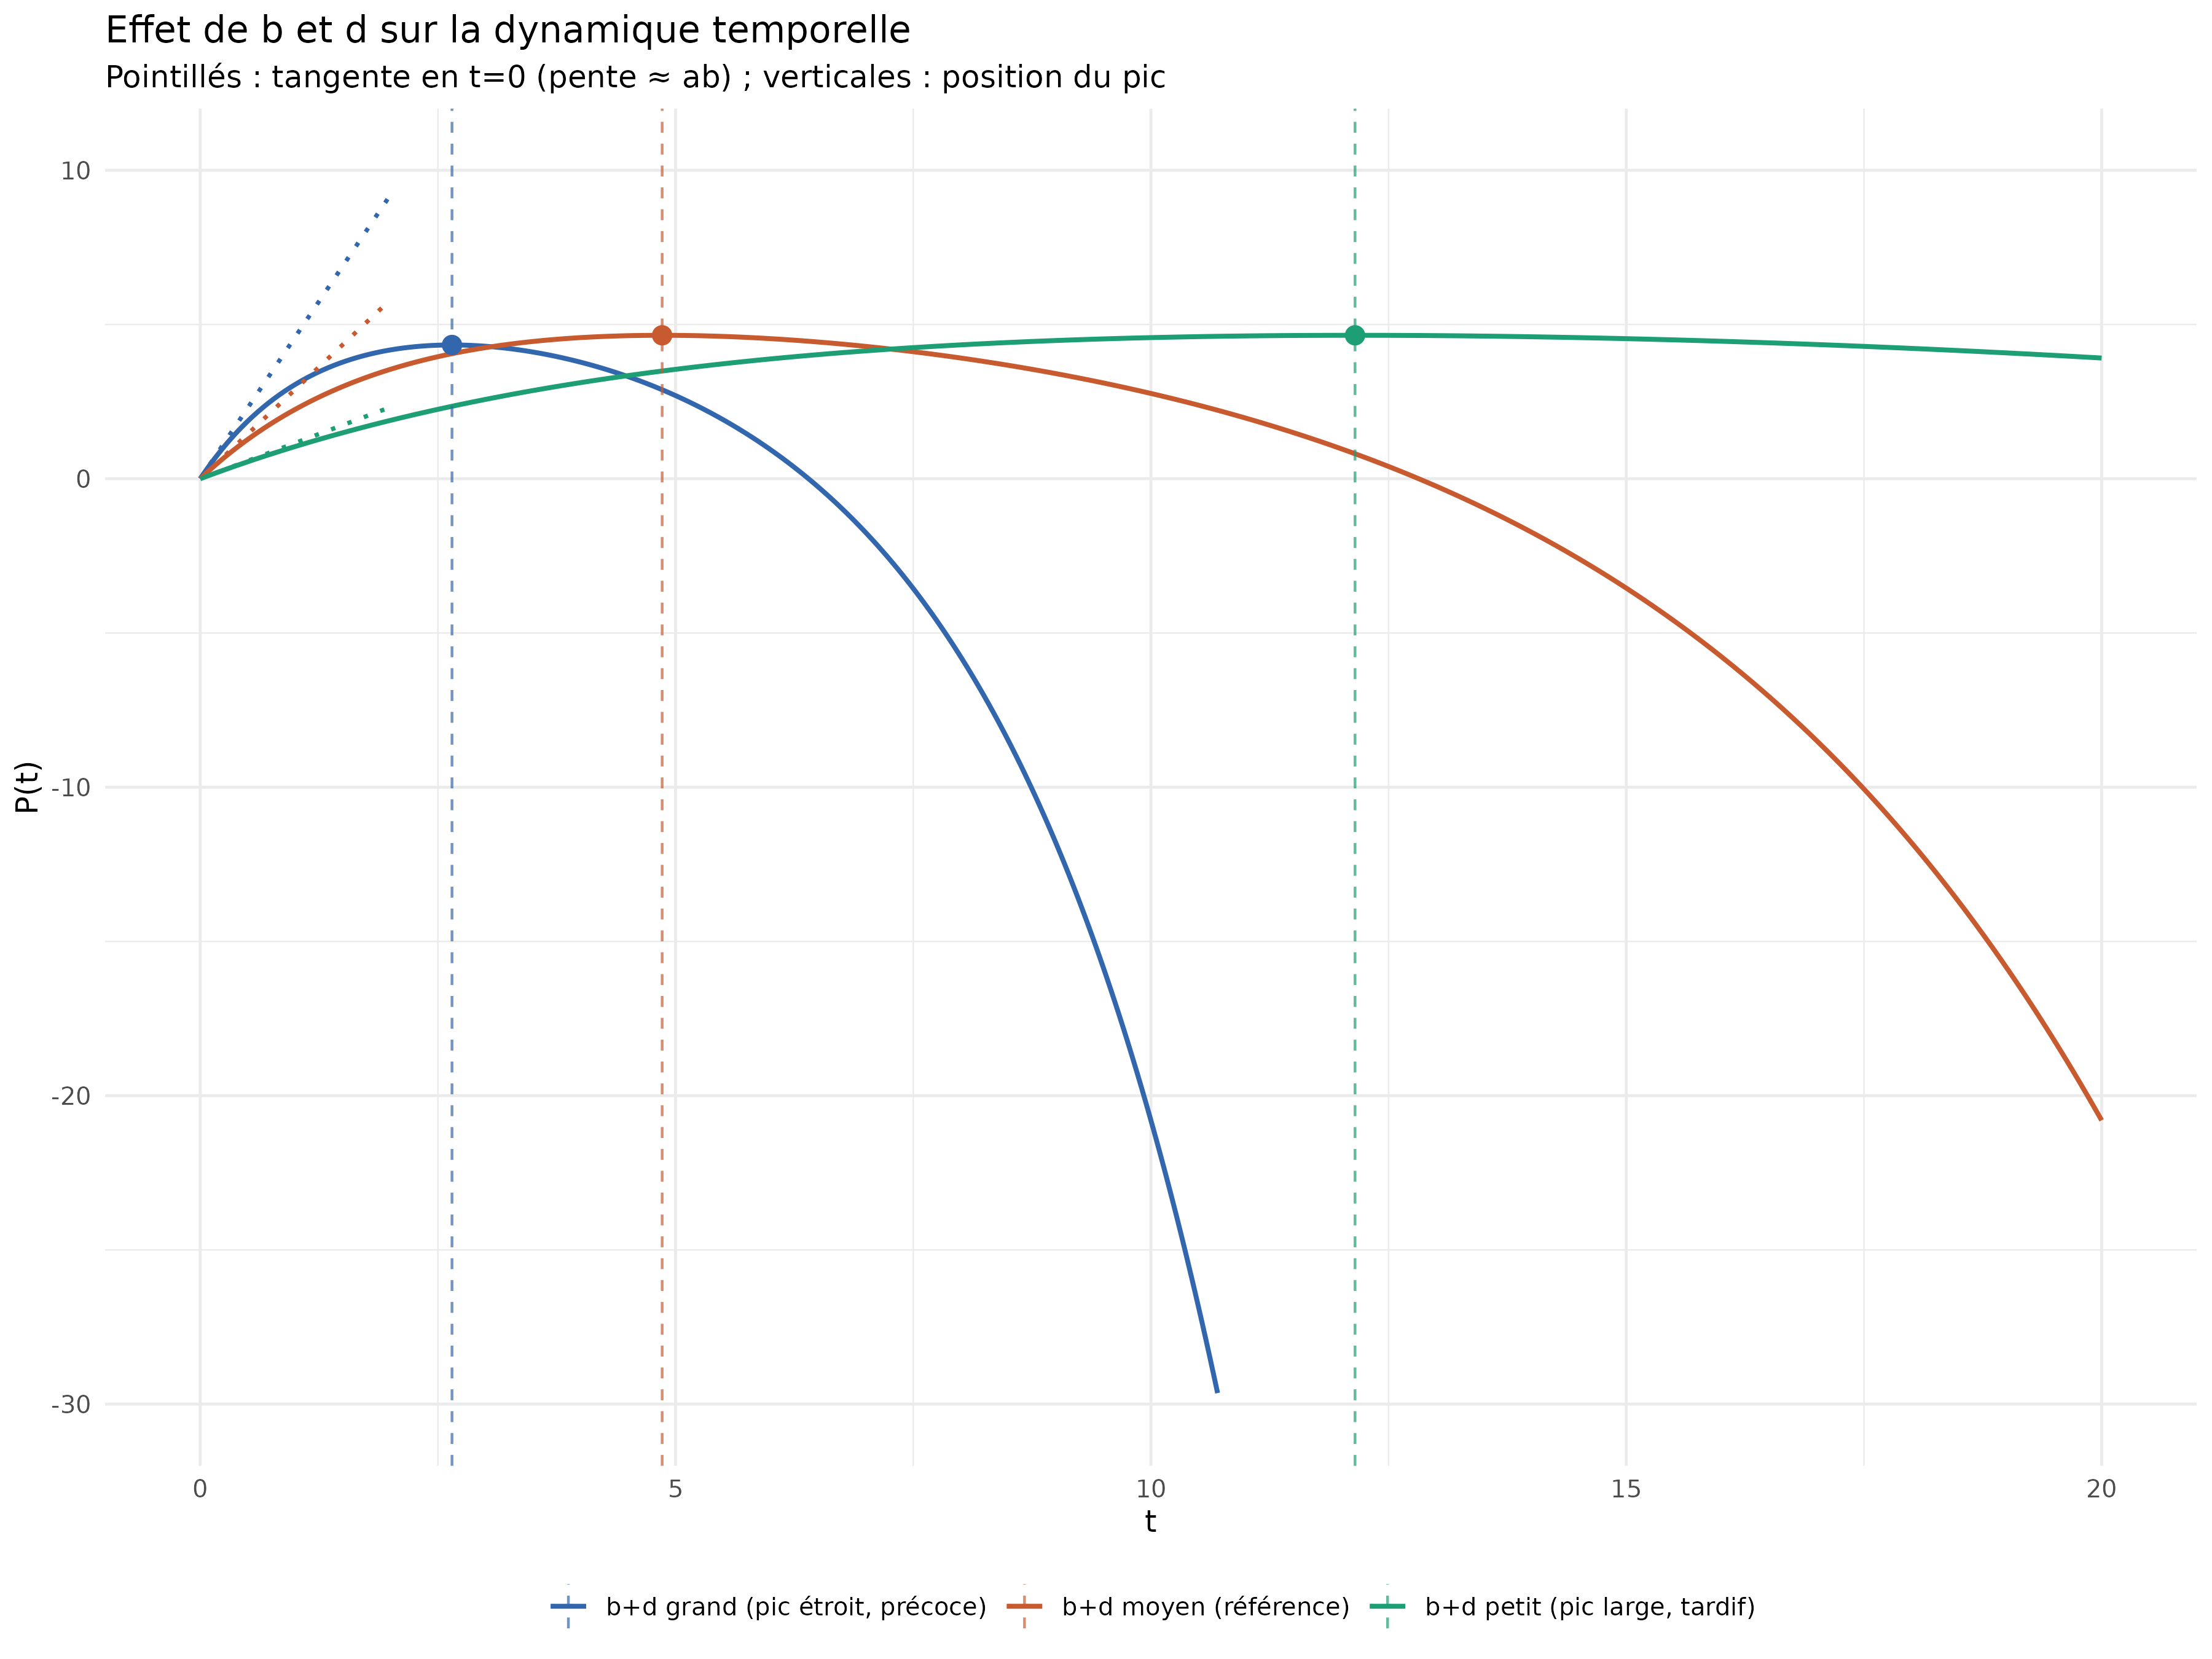
\includegraphics[width=0.8\linewidth,height=\textheight,keepaspectratio]{methodo/b_et_d.png}

}

\caption{Effet de b et d}

\end{figure}%

La position de \(t_{pic}\) a été obtenu en en annulant la dérivée de
P(t). C'est-à-dire en annulant \(P'(t) = ab · e^{−bt} − cd · e^{dt}\),
l'équation \(P'(t) = 0\) traduit l'équilibre instantané entre la vitesse
de montée et la vitesse de descente. Ainsi, cette formule montre que ce
n'est pas a seul ni b seul qui positionnent le pic, mais bien les
produits ab et cd qui s'affrontent dans le rapport R. Sous l'hypothèse c
\textless\textless{} a, on a cd \textless\textless{} ab, donc R
\textgreater\textgreater{} 1, ln(R) \textgreater{} 0 et t* est bien
positif --- le pic existe. Plus c est faible devant a, plus R est grand
et plus le pic est tardif : la descente, peu vigoureuse, tarde à
contrebalancer la montée. À l'inverse, un cas limite instructif est
\(a \cdot b = c \cdot d\), soit \(R = 1\) : \(ln(R) = 0\) et
\(t_{pic} = 0\), il n'y a plus de pic et la courbe est décroissante dès
l'origine. C'est pourquoi la contrainte ab \textgreater{} cd constitue
non seulement une condition de positivité des paramètres, mais bien la
condition d'existence du pic.

\begin{figure}[H]

{\centering 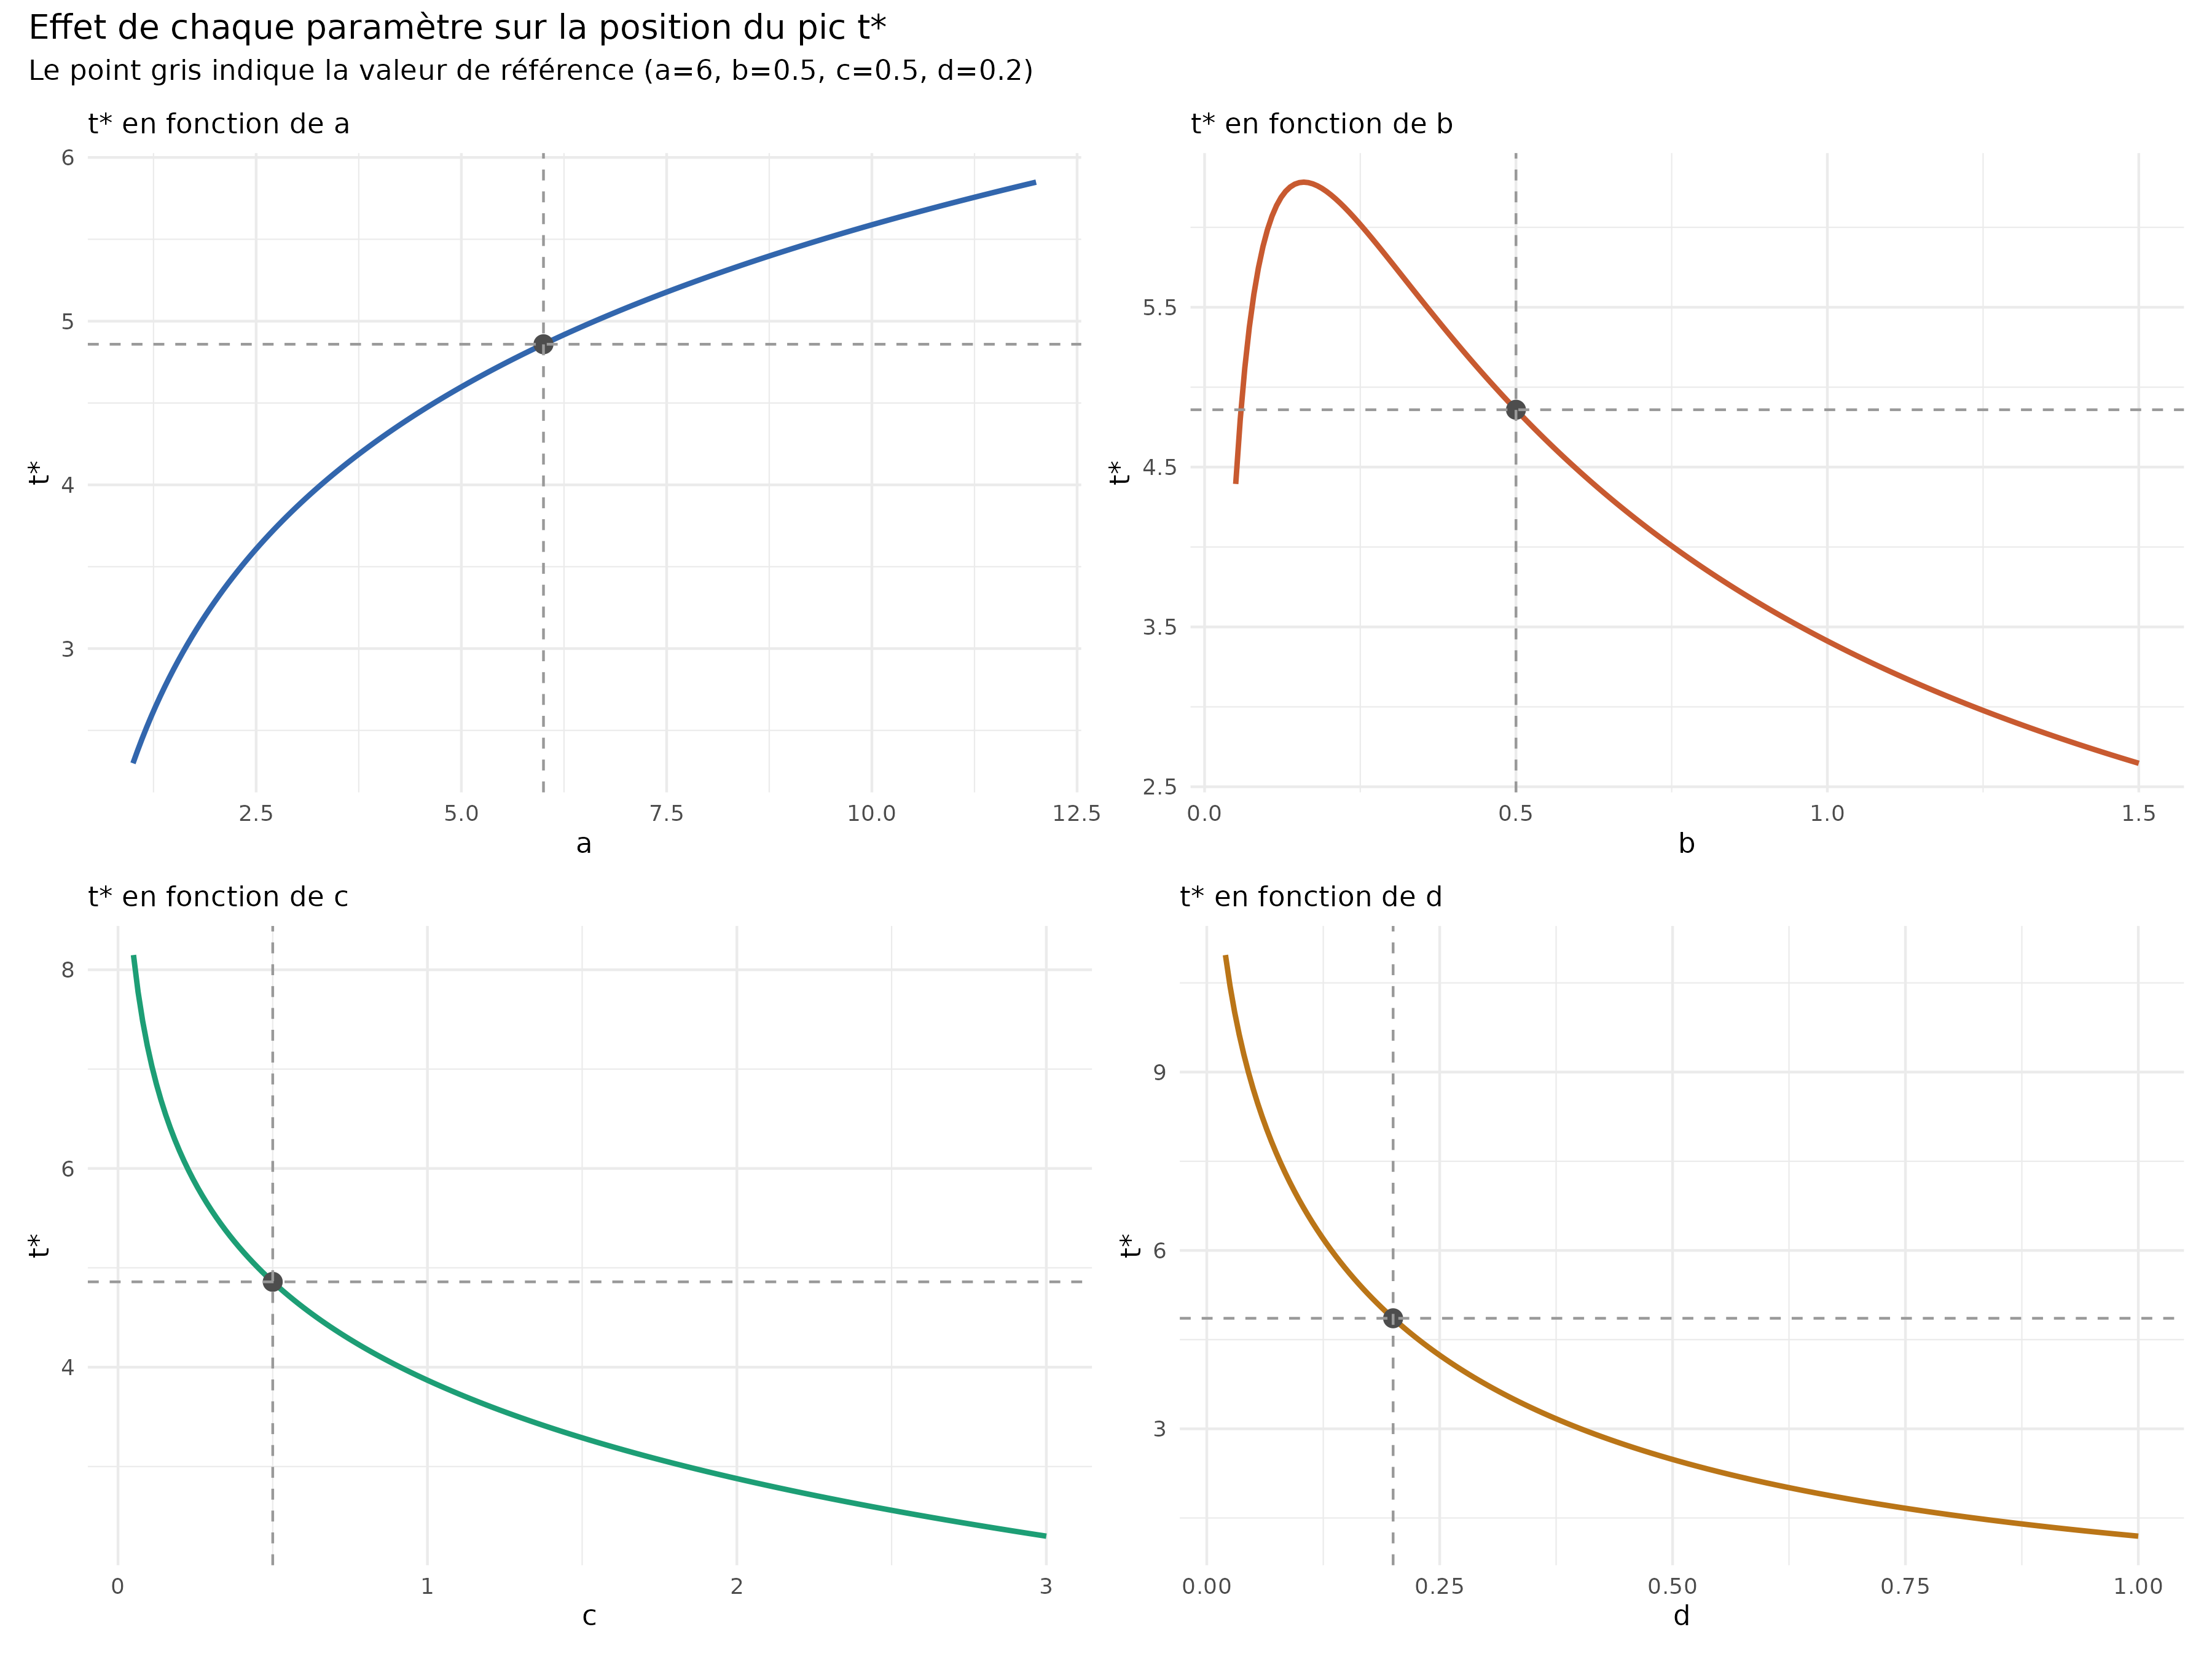
\includegraphics[width=0.8\linewidth,height=\textheight,keepaspectratio]{methodo/effets_params_t_pic.png}

}

\caption{Effet des paramètres sur t\_pic}

\end{figure}%

\subsubsection{Modèle IMAP (2019)}\label{moduxe8le-imap-2019}

Le modèle IMAP (\textit{Integrative Model of Age-Performance}),
développé par Berthelot et al.~en 2019, propose une approche
biologiquement fondée de la relation âge-performance, en modélisant la
dynamique des populations cellulaires au cours de la vie. Contrairement
au modèle de Moore, dont les paramètres sont purement empiriques, l'IMAP
s'appuie sur deux mécanismes cellulaires distincts : la sénescence
réplicative \(\alpha(t)\), qui décrit la croissance puis la saturation
de la population cellulaire, et la perte de fonctionnalité cellulaire
\(\beta(t)\), qui traduit le déclin progressif lié au vieillissement. La
performance \(P(t)\) à l'âge \(t\) est alors donnée par :

\begin{equation}
\label{eq:imap}
P(t) = \beta_0 N_\infty \cdot e^{\frac{\alpha_0}{\alpha_r}(1 - e^{-\alpha_r t})} \cdot \left(1 - e^{\beta_r(t - t_d)}\right)
\end{equation}

où \(N_\infty\) est la taille asymptotique de la population cellulaire,
\(\alpha_0 > 0\) et \(\alpha_r > 0\) contrôlent respectivement le taux
initial et la vitesse de saturation de la croissance cellulaire,
\(\beta_0 > 0\) et \(\beta_r > 0\) contrôlent le taux et la vitesse du
déclin fonctionnel, et \(t_d > 0\) est un paramètre explicite
correspondant à l'âge de décès. Ce dernier paramètre constitue une
différence importante avec le modèle de Moore : il assure une
convergence contrôlée de la courbe et réduit la variabilité des
estimations aux âges avancés.

\subsubsection{Méthode générale}\label{muxe9thode-guxe9nuxe9rale}

\paragraph*{Précautions pour gérer le déséquilibre des
âges}\label{pruxe9cautions-pour-guxe9rer-le-duxe9suxe9quilibre-des-uxe2ges}
\addcontentsline{toc}{paragraph}{Précautions pour gérer le déséquilibre
des âges}

On note dans nos données un fort déséquilibre dans la distribution des
âges (très peu d'âges dits « élevés » et très peu d'âges dit « faibles
»). La figure suivante illustre cela, entre 20 et 30 ans, il y a
beaucoup plus de points qu'avant 20 ans ou après 30 ans. Il va falloir
gérer ce problème car comme chaque point à le même poids, les âges où
nous avons beaucoup de points risquent d'influencer fortement notre
modèle.

\begin{figure}[H]

{\centering 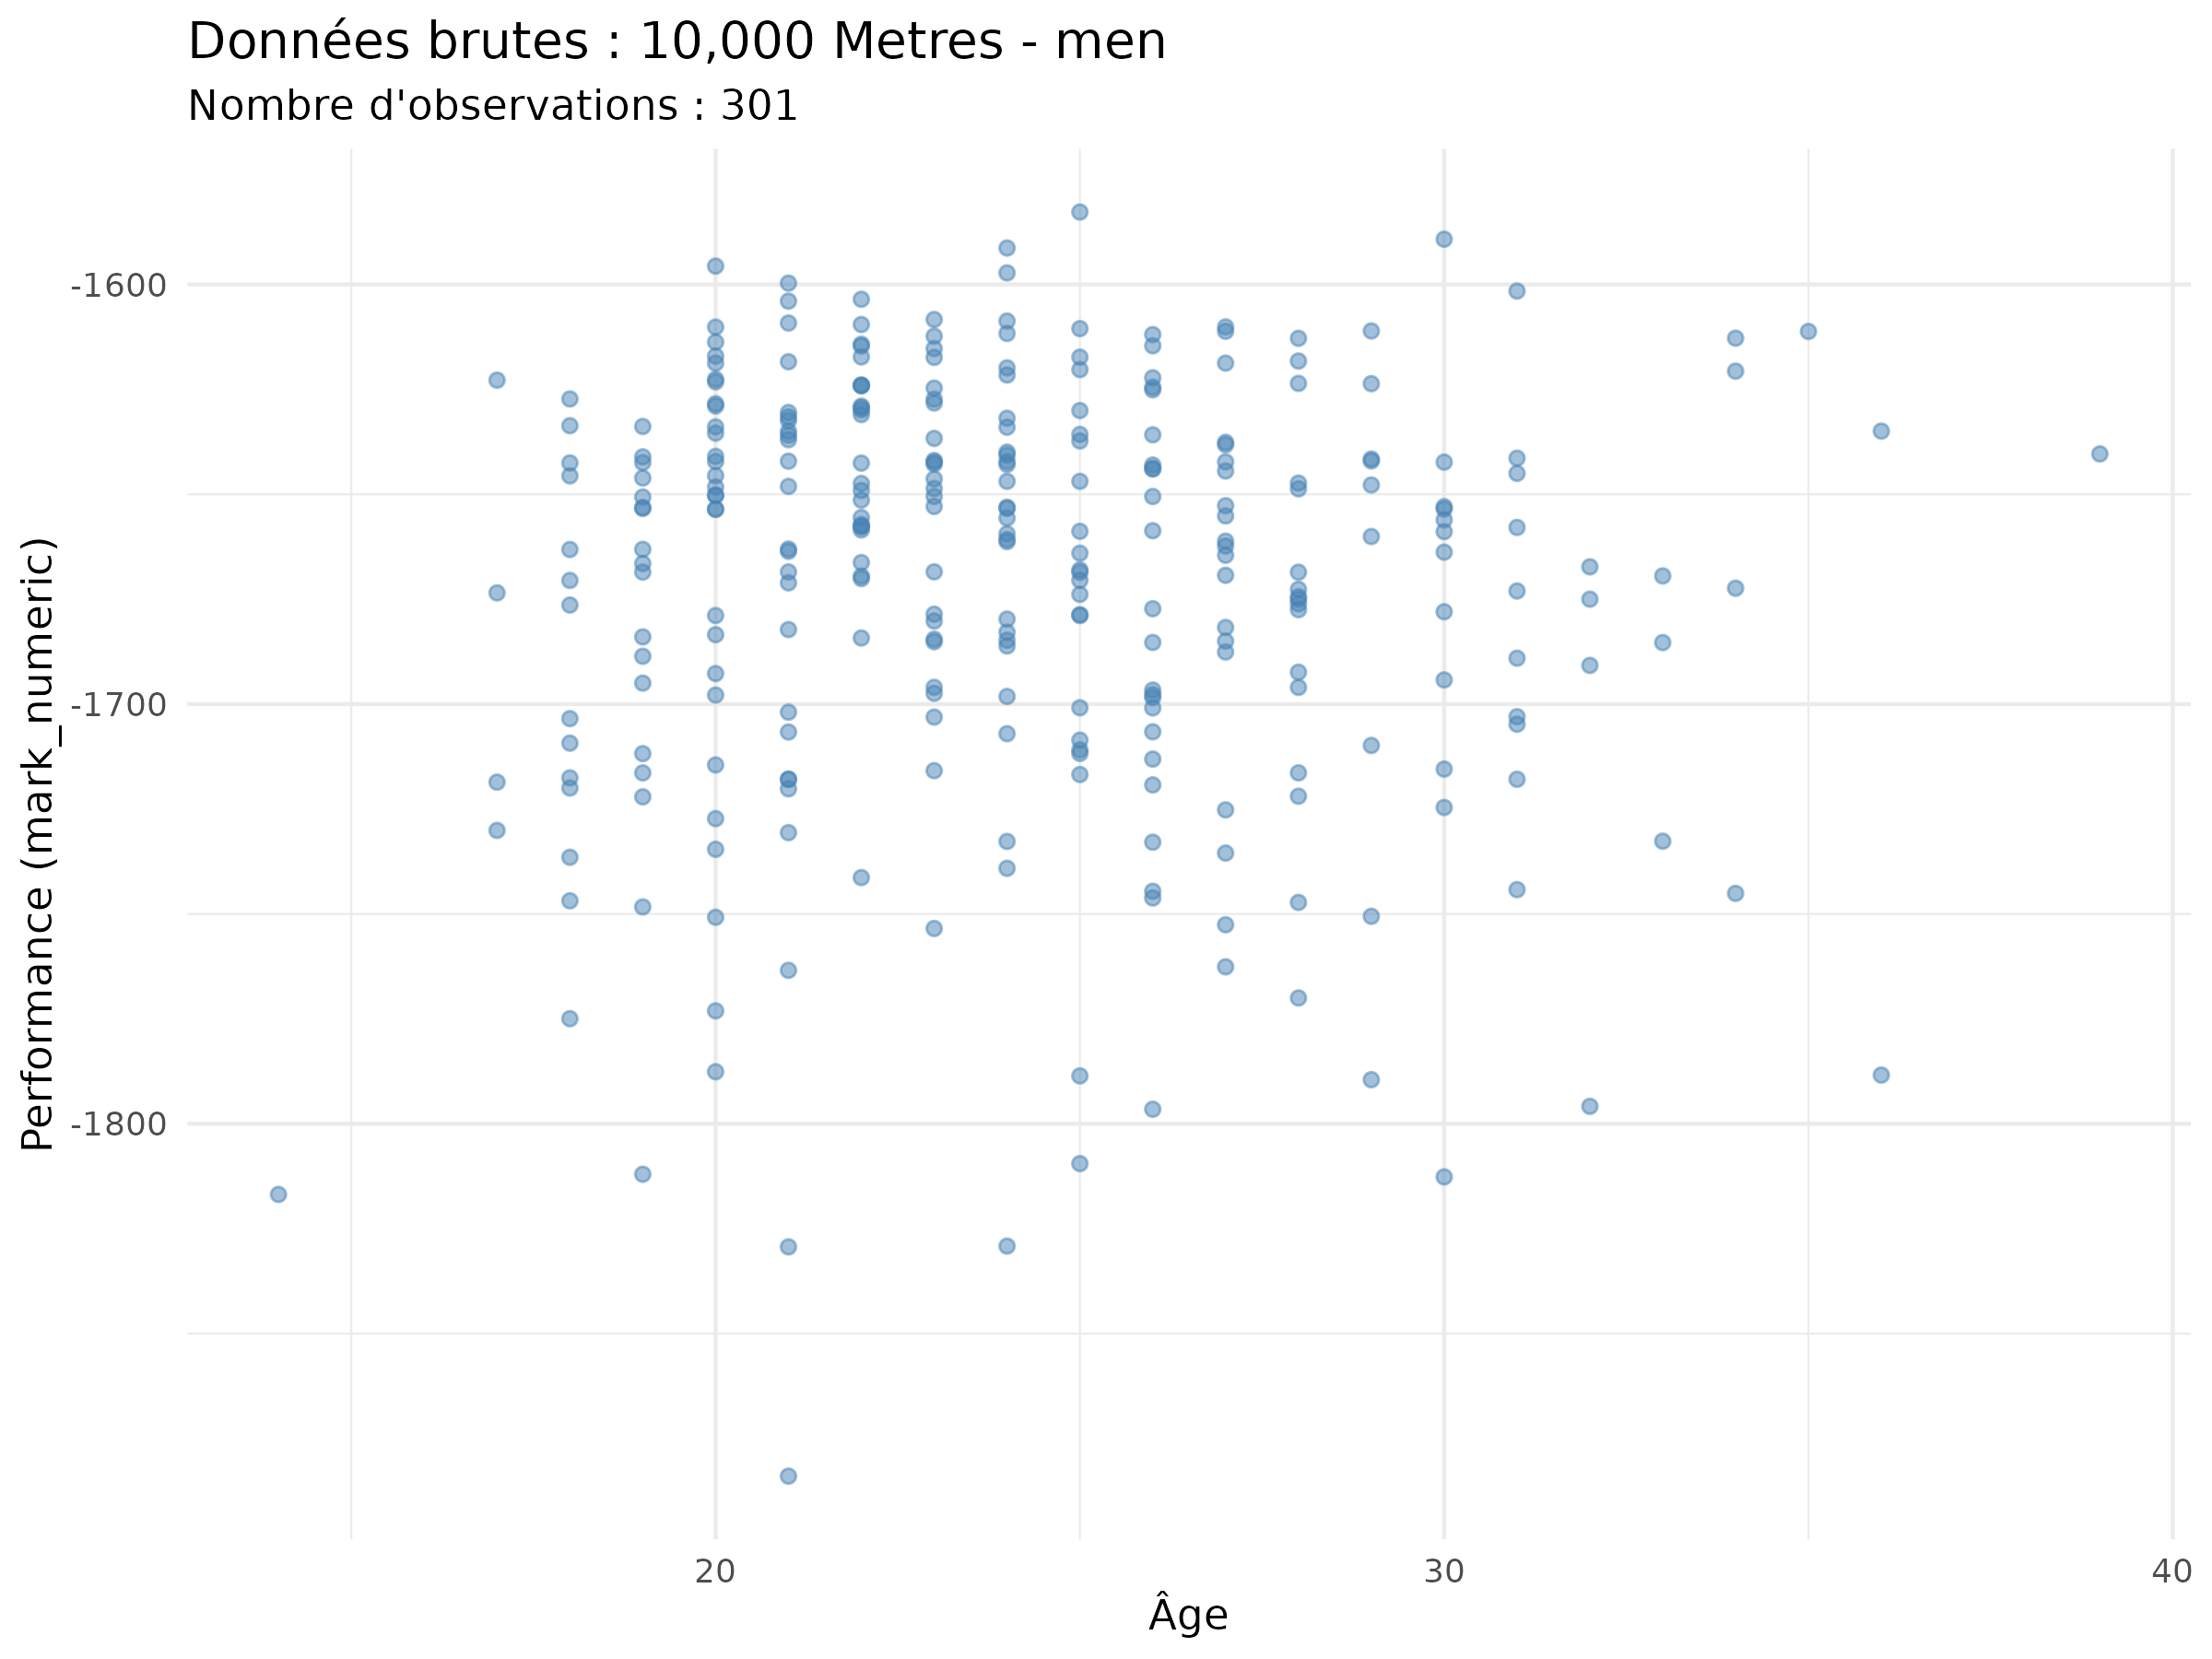
\includegraphics[width=0.8\linewidth,height=\textheight,keepaspectratio]{donnees_reelles_top32/brut_10_000_Metres_men.png}

}

\caption{Top 32}

\end{figure}%

Pour cela, nous allons garder pour chaque âge la meilleure performance
réalisée et estimer nos modèles à partir de ces données.

\begin{figure}[H]

{\centering 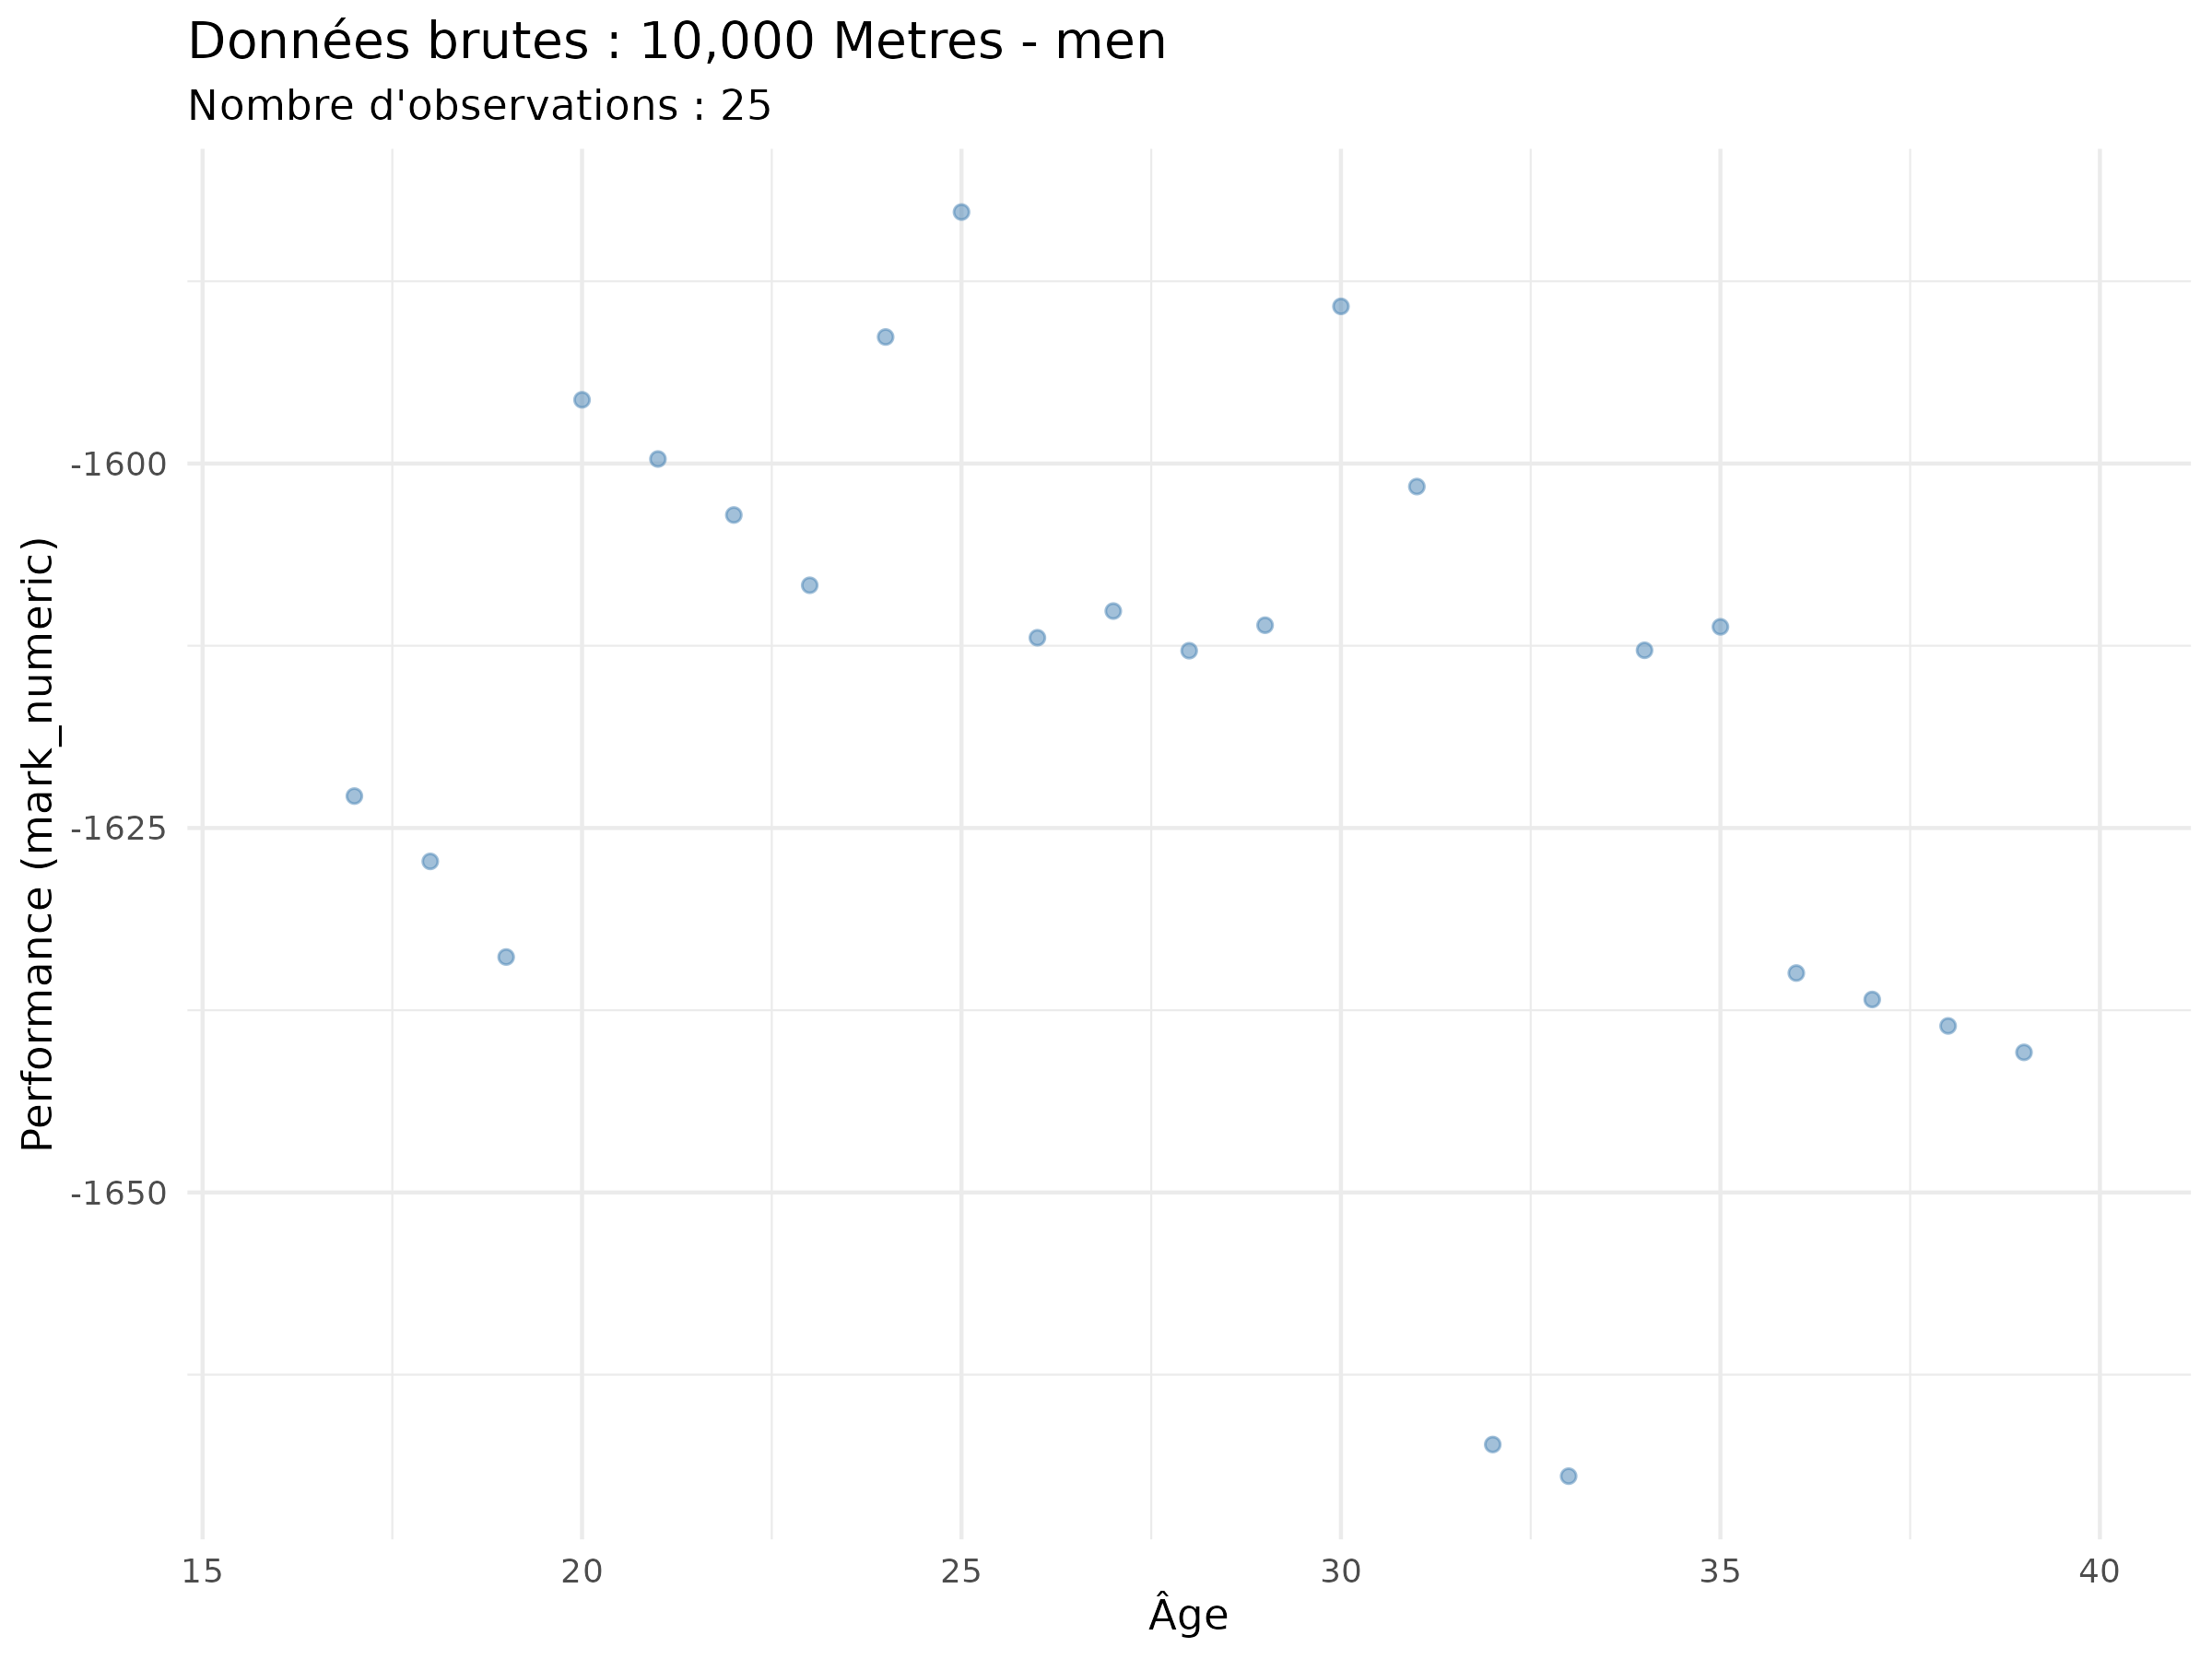
\includegraphics[width=0.8\linewidth,height=\textheight,keepaspectratio]{donnees_reelles_meilleure_par_age/brut_10_000_Metres_men.png}

}

\caption{Meilleure par age}

\end{figure}%

\paragraph*{Descente de gradients}\label{descente-de-gradients}
\addcontentsline{toc}{paragraph}{Descente de gradients}

\subparagraph{Pourquoi cette méthode ?}\label{pourquoi-cette-muxe9thode}

La méthode de la descente de gradient est nécessaire car dans le cadre
du modèle de Moore comme pour le modèle IMAP, les formules présentent
une non-linéarité par rapport à certains paramètres. La non-linéarité
est selon les paramètres b et d, situés en exposants pour le modèle de
Moore et selon les paramètres \(\alpha_r\), \(\beta_r\) et \(\alpha_0\).
Contrairement à une régression linéaire classique (MCO), il n'existe pas
de formule explicite permettant de calculer directement les coefficients
optimaux par une simple inversion matricielle. La structure même de
l'équation, composée de deux membres bi-exponentiels, crée une
interdépendance forte : il devient difficile d'isoler l'influence de
chaque partie sur l'allure globale de la courbe, car les deux termes
``se mélangent'' pour produire le résultat final. Là où une régression
linéaire tenterait de trouver une solution globale et instantanée, la
descente de gradient adopte une approche plus fine et progressive. Elle
ajuste les paramètres et de concert, avançant pas à pas dans toutes les
directions pour minimiser l'erreur, permettant ainsi de calibrer
précisément le modèle là où les méthodes directes échouent.

\subparagraph{Fonctionnement}\label{fonctionnement}

La descente de gradient est un algorithme d'optimisation itératif du
premier ordre. Son objectif est de déterminer le jeu de paramètres
\(\theta={\theta_1, ...,\theta_n}\) qui minimise une fonction de coût
(ou fonction de perte), notée \(J(\theta)\). Dans ce cadre, nous
utilisons l'Erreur Quadratique Moyenne (MSE), qui mesure l'écart entre
les prédictions du modèle et les observations réelles. Le gradient, noté
\(\nabla J(\theta)\), est le vecteur regroupant les dérivées partielles
de la fonction de coût par rapport à chaque paramètre :
\[\nabla J(\theta) = \begin{pmatrix} \frac{\partial J}{\partial \theta_1} \\ \vdots \\ \frac{\partial J}{\partial \theta_n} \end{pmatrix}\]
Mathématiquement, ce vecteur pointe toujours vers la direction de la
plus forte augmentation de la fonction. Par conséquent, pour minimiser
l'erreur, l'algorithme doit se déplacer dans la direction opposée au
gradient. L'algorithme démarre d'une initialisation arbitraire et met à
jour les paramètres de manière itérative selon la règle suivante :
\(\theta_{next} = \theta_{current} – \eta \cdot \nabla J(\theta)\). Dans
cette formule, \(\eta\) représente le taux d'apprentissage (learning
rate). C'est un hyperparamètre crucial qui détermine la taille du pas
effectué à chaque étape : - S'il est trop grand, l'algorithme risque
d'osciller et de ne jamais converger. - S'il est trop petit, la
progression sera extrêmement lente. L'opération est répétée jusqu'à la
convergence, c'est-à-dire lorsque le gradient devient proche de zéro
(indiquant que nous avons atteint un minimum) ou lorsque le nombre
maximal d'itérations est atteint.

\subparagraph{Optimum local}\label{optimum-local}

La descente de gradient est une méthode permettant d'obtenir un optimum
local qu'il faut distinguer de l'optimum global. En effet, l'optimum
local dépend du point d'où nous décidons de partir et n'est pas
forcément le meilleur optimum. Dans cette méthode, le point de départ
choisi joue donc un rôle essentiel et a une influence considérable sur
les paramètres estimés. Pour contrer ce problème, nous allons estimer
plusieurs modèles (1000) pour chaque couple (Sex, discipline) en
générant de façon aléatoire les points de départ pour chacune des
estimations.

\begin{figure}[H]

{\centering 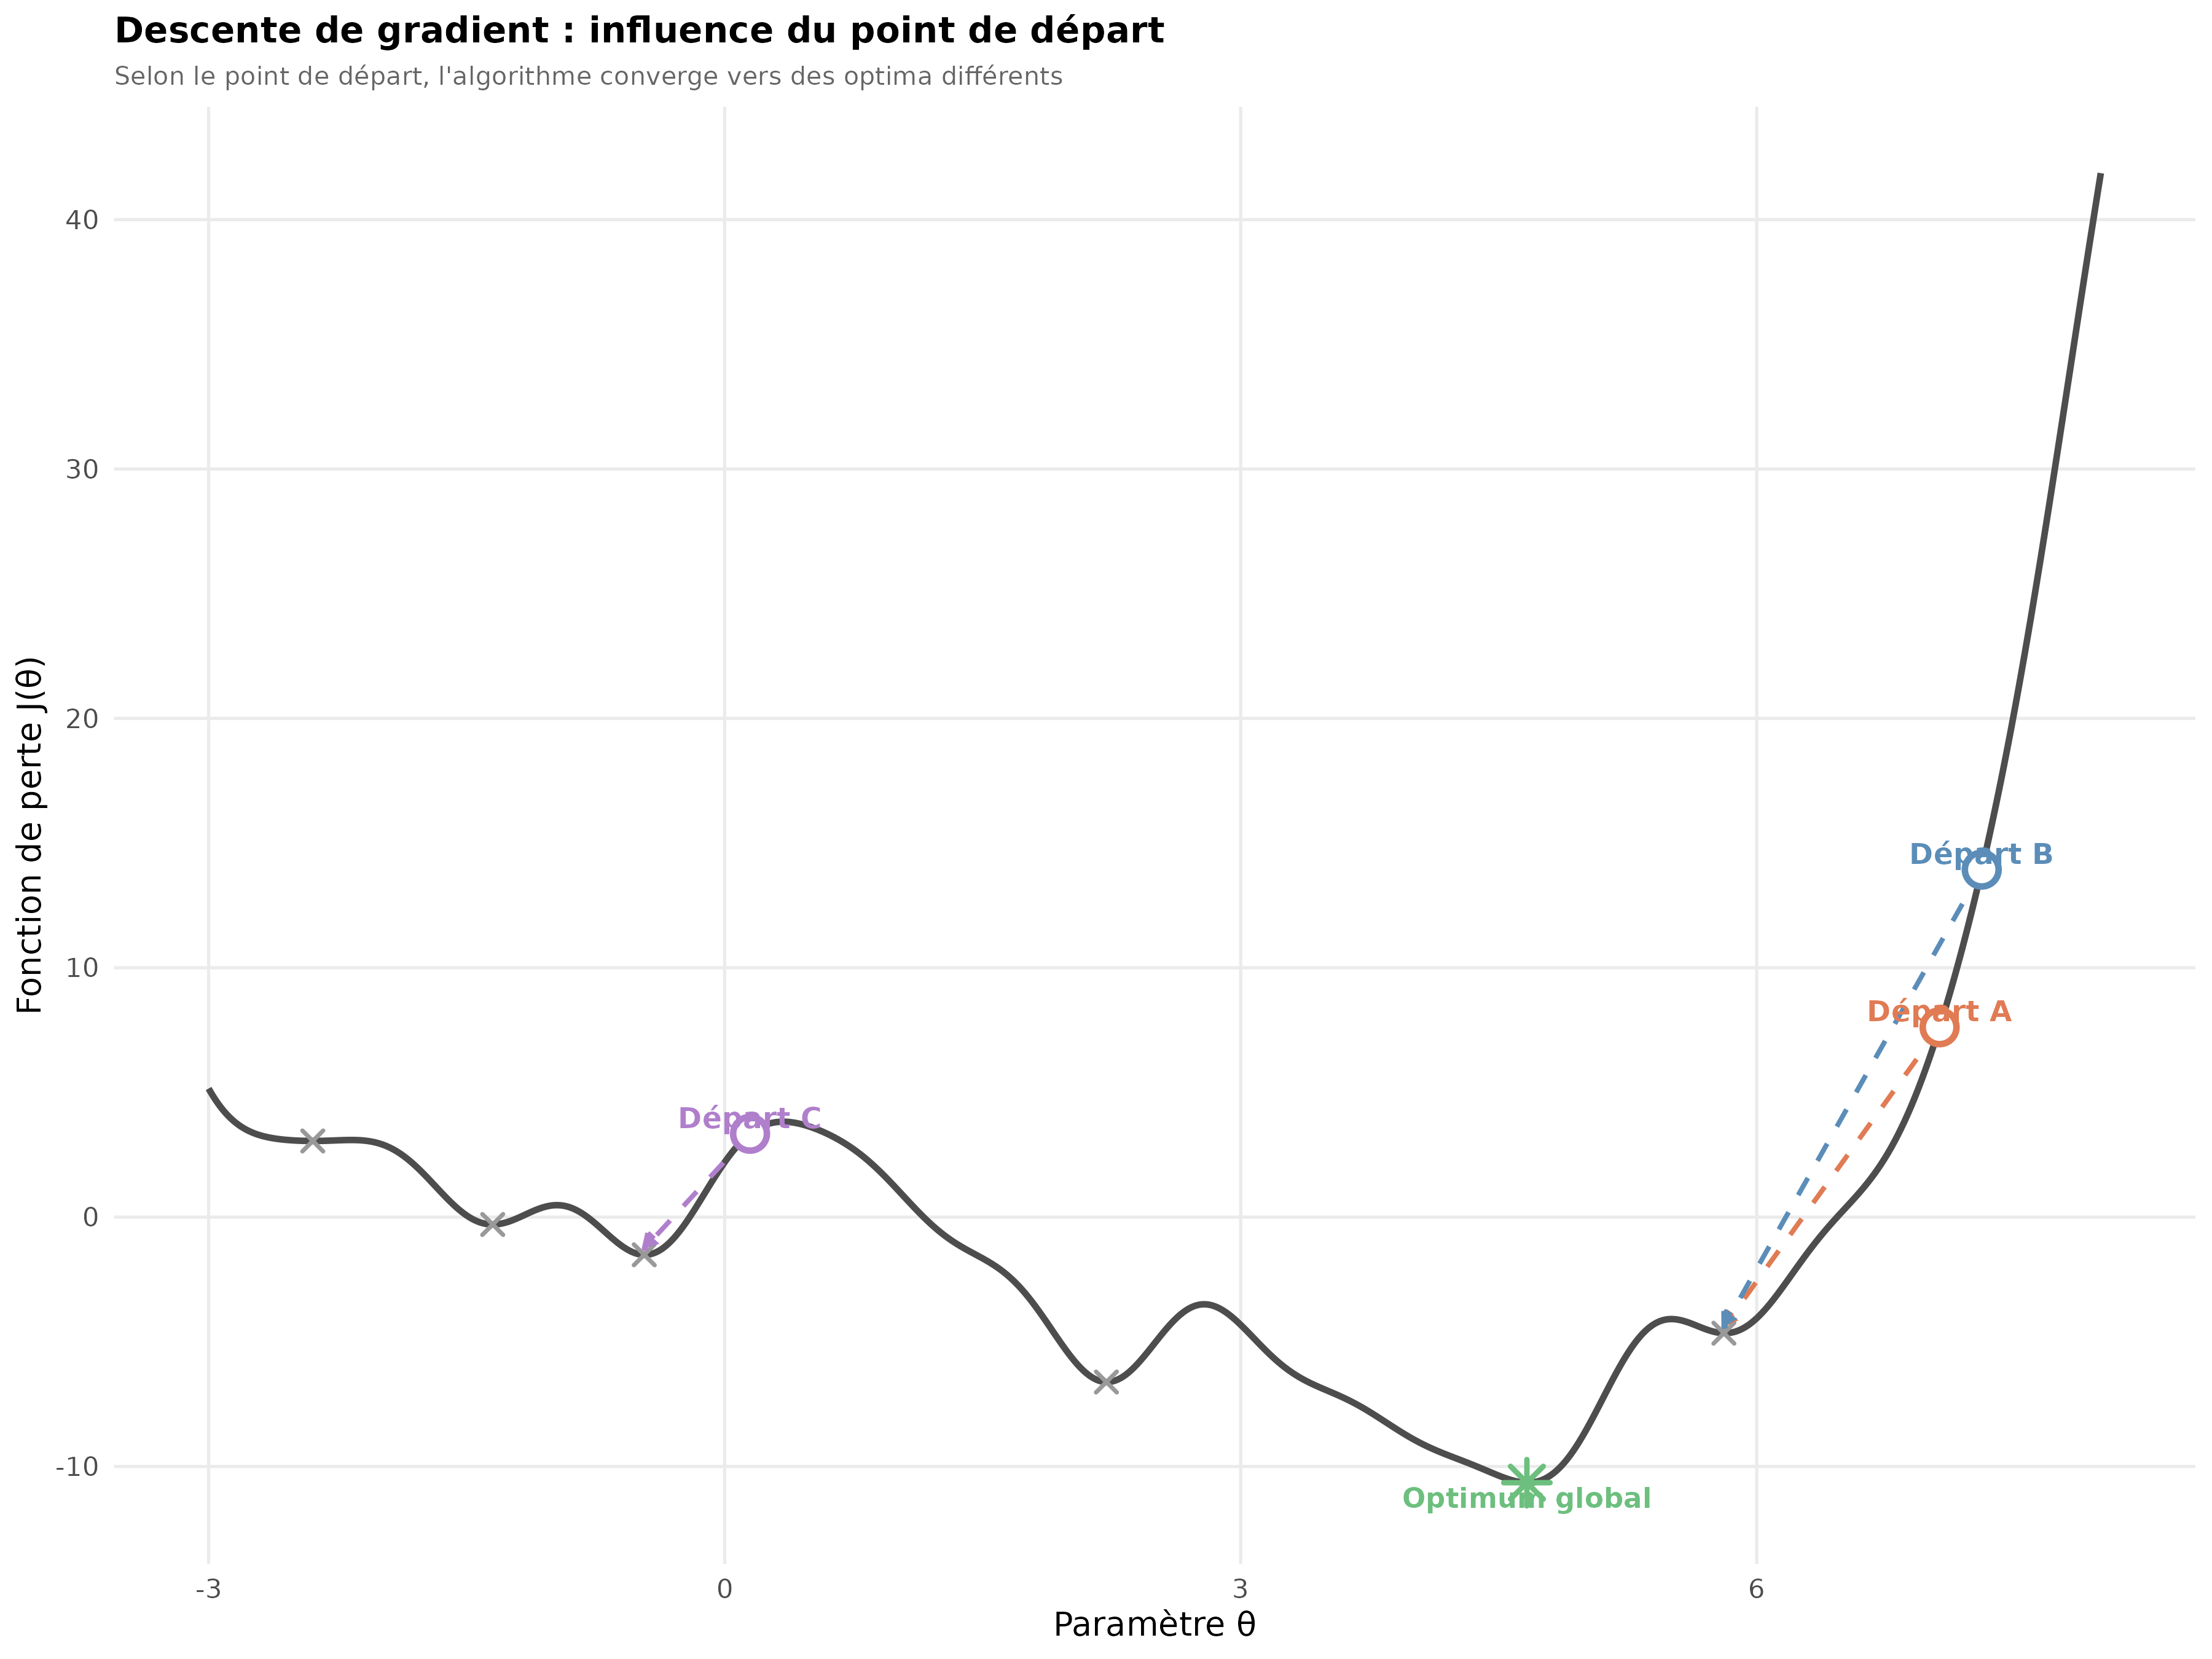
\includegraphics[width=0.8\linewidth,height=\textheight,keepaspectratio]{methodo/descente_gradient.png}

}

\caption{Optimum local et descente de graident}

\end{figure}%

\paragraph*{Introduction de
l'aléatoire}\label{introduction-de-laluxe9atoire}
\addcontentsline{toc}{paragraph}{Introduction de l'aléatoire}

Le point de départ choisi jouant un rôle essentiel dans la détermination
des paramètres estimés, il est essentiel d'ajouter une part d'aléatoire
dans le choix de ces paramètres. Ainsi nous estimerons plusieurs fois
chaque modèle avec des points de départ généré aléatoirement à chaque
fois. Nous allons ainsi estimés 1 000 modèles pour chaque couple afin de
maximiser nos chances d'en avoir qui convergent et pouvoir ensuite
choisir le plus performant.

\subparagraph{L'aléatoire dans le modèle de
Moore}\label{laluxe9atoire-dans-le-moduxe8le-de-moore}

Initialisation des paramètres du modèle

Afin d'estimer les paramètres du modèle de Moore, nous devons fournir à
l'algorithme de descente de gradient des valeurs initiales pour
\(a, b, c\) et \(d\). Celles-ci sont générées aléatoirement à partir des
propriétés observables de la série de données, selon le schéma suivant :

\begin{itemize}
\tightlist
\item
  \textbf{\(a\)} est tiré uniformément entre 0,9 et 1,2 fois la valeur
  de performance maximale observée, reflétant le fait que le plateau
  asymptotique du terme montant est légèrement supérieur au pic ;
\item
  \textbf{\(b\)} est tiré uniformément autour du rapport
  \(\frac{\text{pente initiale}}{a}\), conformément à l'approximation
  \(f'(0) \approx ab\) valable lorsque \(c \ll a\) ;
\item
  \textbf{\(c\)} est tiré uniformément dans un voisinage étroit de
  \(a/100\), traduisant l'hypothèse que le terme descendant est une
  petite perturbation devant le terme montant ;
\item
  \textbf{\(d\)} est tiré uniformément autour de l'estimateur
  \(\frac{\ln[(f(t_3) - a) / (f(t_4) - a)]}{t_3 - t_4}\), obtenu par
  régression sur deux points situés dans la phase descendante de la
  courbe.
\end{itemize}

Par ailleurs, les quatre paramètres étant par définition strictement
positifs, des contraintes de positivité sont imposées lors de la
génération, sans restriction sur les valeurs maximales.

\subparagraph*{Adaptation du modèle IMAP à nos
données}\label{adaptation-du-moduxe8le-imap-uxe0-nos-donnuxe9es}
\addcontentsline{toc}{subparagraph}{Adaptation du modèle IMAP à nos
données}

Le modèle IMAP tel que proposé par Berthelot et al.~(2019) a été conçu
pour des données couvrant l'ensemble du cycle de vie, de 5 à 75 ans
environ. Dans ce cadre, les six paramètres --- \(\alpha_0\),
\(\alpha_r\), \(\beta_0\), \(N_\infty\), \(\beta_r\) et \(t_d\) --- sont
tous identifiables car la courbe présente à la fois une phase de
croissance complète, un pic prononcé et une phase de déclin étendue.

Notre jeu de données couvre en revanche une fenêtre beaucoup plus
restreinte, de 16 à 40 ans, correspondant aux carrières des athlètes
d'élite. Cette troncature crée un problème d'\textbf{identifiabilité} :
les paramètres \(\beta_0\) et \(N_\infty\) n'apparaissant que sous forme
de produit dans la formule, ils ne peuvent pas être estimés séparément.
Ils ont donc été fusionnés en un unique paramètre d'amplitude
\(A = \beta_0 N_\infty\), ramenant le nombre de paramètres libres à
quatre : \(A\), \(\alpha_0\), \(\alpha_r\) et \(\beta_r\). La formule
estimée est ainsi :

\[P(t) = A \cdot e^{\frac{\alpha_0}{\alpha_r}(1 - e^{-\alpha_r t})}
\cdot \left(1 - e^{\beta_r(t - t_d)}\right)\]

\subparagraph*{\texorpdfstring{Choix du paramètre
\(t_d\)}{Choix du paramètre t\_d}}\label{choix-du-paramuxe8tre-t_d}
\addcontentsline{toc}{subparagraph}{Choix du paramètre \(t_d\)}

Le paramètre \(t_d\), qui représente dans le modèle original l'espérance
de vie de l'athlète, ne peut pas être estimé de façon fiable sur des
données tronquées à 40 ans : la phase de déclin terminal est trop peu
visible dans la fenêtre d'observation pour contraindre ce paramètre. Des
tests ont confirmé que laisser \(t_d\) libre conduit systématiquement à
une matrice de gradient singulière et à l'absence de convergence.

Nous avons donc fixé \(t_d\) à une valeur supérieure à l'âge maximal
observé dans chaque groupe (discipline \(\times\) sexe), en testant huit
valeurs : \(t_d = \max(\text{Age}) + \delta\) avec
\(\delta \in \{10, 15, 20, 25, 30,
35, 40, 45\}\). Pour chaque valeur de \(\delta\), 500 estimations sont
lancées avec des points de départ aléatoires, et la valeur retenue est
celle qui minimise le RMSE sur l'ensemble des huit candidats.

Cette approche garantit que le terme de déclin est suffisamment visible
dans la fenêtre d'observation pour que le gradient soit non singulier,
tout en restant cohérente avec l'interprétation de \(t_d\) comme horizon
temporel au-delà duquel la performance décline rapidement. Il convient
de noter que \(t_d\) ne représente plus ici l'âge de décès biologique au
sens strict, mais un paramètre de calibration lié à la fenêtre des
données.

\subparagraph{L'aléatoire dans le modèle
IMAP}\label{laluxe9atoire-dans-le-moduxe8le-imap}

Comme pour le modèle de Moore, le problème des optima locaux est géré
par une procédure de départs multiples aléatoires. Les points de départ
des quatre paramètres libres sont générés aléatoirement à chaque
itération, selon une logique proportionnelle à \(t_d\) inspirée des
travaux de Berthelot et al.~(2019) :

\begin{itemize}
  \item $A$ est tiré négativement dans l'intervalle
        $[-0{,}003 \cdot t_d \;;\; -0{,}002 \cdot t_d]$,
        reflétant le fait que le terme de déclin impose $A < 0$ pour que
        la courbe reste positive sur la fenêtre d'observation ;
  \item $\alpha_0$ est tiré dans
        $[0{,}00075 \cdot t_d \;;\; 0{,}00325 \cdot t_d]$ ;
  \item $\alpha_r$ est tiré dans
        $[0{,}00225 \cdot t_d \;;\; 0{,}00325 \cdot t_d]$ ;
  \item $\beta_r$ est tiré négativement dans
        $[-0{,}0015 \cdot t_d \;;\; -0{,}0005 \cdot t_d]$.
\end{itemize}

Pour chaque valeur de \(t_d\) testée, 500 modèles sont estimés et le
meilleur --- au sens du RMSE --- est retenu. Au total, 4 000 estimations
sont donc réalisées par couple (sexe \(\times\) discipline).

\paragraph*{Choix du modèle le plus performant : Critère
d'optimisation}\label{choix-du-moduxe8le-le-plus-performant-crituxe8re-doptimisation}
\addcontentsline{toc}{paragraph}{Choix du modèle le plus performant :
Critère d'optimisation}

Une fois les modèles estimés, il va nous falloir déterminer les
paramètres optimaux pour chaque modèle afin de résumer au mieux les
données et obtenir une courbe la plus représentative possible. Il nous
faut donc un critère d'optimisation. Le critère d'optimisation que nous
allons utiliser est assez classique : il s'agit de l'erreur quadratique
(ou méthode des moindres carrés). Ce critère consiste à minimiser la
somme des erreurs quadratiques, notée :
\[S(\theta) = \sum_{i=1}^{N} (f_i - \hat{f}(age_i, \theta))^2\] On
cherche donc :
\[\arg\min_{\theta} \sum_{i=1}^{N} (f_i - \hat{f}(age_i, \theta))^2\].

Pour chaque couple (sexe, discipline), nous allons choisir parmi les
différents modèles estimés (et ayant donc convergés) celui qui MSE. On
trouve ainsi les paramètres correspondant au modèle le plus performant.

\paragraph*{Comparaison des modèles : AIC et
BIC}\label{comparaison-des-moduxe8les-aic-et-bic}
\addcontentsline{toc}{paragraph}{Comparaison des modèles : AIC et BIC}

Afin de comparer les différents modèles de régression linéaire
considérés dans cette étude, les critères d'information AIC (Akaike
Information Criterion) et BIC (Bayesian Information Criterion) sont
utilisés. Ces deux critères reposent sur une logique commune : pénaliser
la complexité du modèle afin d'éviter le surapprentissage, tout en
cherchant à minimiser l'erreur de prévision sur de nouvelles
observations.

\subparagraph{AIC : Akaike Information
Criterion}\label{aic-akaike-information-criterion}

L'AIC est défini par \[AIC=n \cdot \ln(\frac {SRC} n)+2(p+1)\] où n
désigne le nombre d'observations, p le nombre de variables explicatives
retenues dans le modèle, et SCR la somme des carrés des résidus. Cette
formule, valable sous hypothèse de normalité des erreurs, quantifie
l'erreur de prévision via la divergence de Kullback-Leibler.

\subparagraph{BIC : Bayesian Information
Criterion}\label{bic-bayesian-information-criterion}

Le BIC est quant à lui défini par
\[BIC=n \cdot \ln(\frac {SRC} n)+(p+1) \cdot \ln (n),\] et se distingue
de l'AIC uniquement par le remplacement du facteur 2 par \[\ln (n)\]
dans le terme de pénalité. Bien que proches dans leur formulation, ces
deux critères conduisent fréquemment au choix de modèles différents.

Pour chacun de ces critères, le modèle retenu est celui présentant la
valeur la plus faible.

\subsection{Résultats}\label{ruxe9sultats-1}

\subsubsection*{Résultats du modèle
IMAP}\label{ruxe9sultats-du-moduxe8le-imap}
\addcontentsline{toc}{subsubsection}{Résultats du modèle IMAP}

Le modèle IMAP a convergé pour l'ensemble des 42 couples (sexe
\(\times\) discipline). Le Tableau 4 présente les âges au pic estimés
par groupe de disciplines.

\begin{longtable}[]{@{}lllll@{}}
\caption{Âge au pic estimé par le modèle IMAP selon le groupe de
disciplines et le sexe}\label{tbl-imap-groupes}\tabularnewline
\toprule\noalign{}
Groupe & Sexe & \(t_{\text{pic}}\) moyen & Min & Max \\
\midrule\noalign{}
\endfirsthead
\toprule\noalign{}
Groupe & Sexe & \(t_{\text{pic}}\) moyen & Min & Max \\
\midrule\noalign{}
\endhead
\bottomrule\noalign{}
\endlastfoot
Sprint & Hommes & 27,1 & 25,3 & 29,2 \\
Sprint & Femmes & 27,3 & 26,8 & 28,2 \\
Haies & Hommes & 27,0 & 26,9 & 27,0 \\
Haies & Femmes & 27,2 & 26,4 & 28,0 \\
Demi-fond & Hommes & 26,6 & 25,2 & 27,7 \\
Demi-fond & Femmes & 26,1 & 24,9 & 27,1 \\
Fond & Hommes & 25,2 & 24,9 & 25,4 \\
Fond & Femmes & 27,0 & 25,8 & 28,3 \\
Marathon & Hommes & 29,5 & 29,5 & 29,5 \\
Marathon & Femmes & 29,8 & 29,8 & 29,8 \\
Marche & Hommes & 28,2 & 28,2 & 28,2 \\
Marche & Femmes & 27,3 & 27,3 & 27,3 \\
Lancers & Hommes & 28,6 & 26,8 & 30,0 \\
Lancers & Femmes & 27,6 & 27,2 & 28,3 \\
Sauts & Hommes & 27,2 & 26,3 & 28,4 \\
Sauts & Femmes & 27,9 & 27,0 & 28,7 \\
Combinées & Hommes & 26,6 & 26,6 & 26,6 \\
Combinées & Femmes & 25,3 & 25,3 & 25,3 \\
\end{longtable}

Les estimations se situent entre 25 et 30 ans pour la majorité des
groupes. Le marathon constitue l'exception la plus nette, avec un pic
estimé à 29,5 ans chez les hommes et 29,8 ans chez les femmes. Les
différences entre sexes sont faibles : les femmes présentent un pic
légèrement plus tardif dans les sauts (+0,7 an en moyenne) et au
marathon (+0,3 an), mais légèrement plus précoce dans les épreuves de
fond et les épreuves combinées, avec des écarts restant dans une marge
de 1 à 2 ans.Concernant la qualité d'ajustement, le RMSE varie selon
l'unité de mesure de la performance : les disciplines exprimées en
mètres (lancers, RMSE moyen de 1,57 m chez les hommes) présentent des
erreurs absolues plus élevées que les disciplines exprimées en km/h
(marche athlétique, RMSE \textless{} 0,01).

\paragraph{exemple du marathon}\label{exemple-du-marathon}

La figure Figure~\ref{fig-imap-marathon} présente les ajustements
obtenus pour les marathoniens et marathoniennes du Top 39. Chez les
hommes, le modèle estime un pic de performance à \textbf{29,5 ans}, avec
un \(t_d\) retenu de 65 ans. La courbe capture la phase de progression
entre 18 et 28 ans, le plateau autour de 29--31 ans, puis le déclin
progressif jusqu'à 40 ans. Chez les femmes, le pic estimé est légèrement
plus tardif à \textbf{29,8 ans}, avec un \(t_d\) retenu de 85 ans. La
dispersion des points est plus importante que chez les hommes ---
notamment une performance à 35 ans (18,49 km/h) s'écartant nettement de
la tendance centrale --- ce qui se traduit par un RMSE légèrement plus
élevé (0,20 km/h) et des critères AIC et BIC moins favorables.

\begin{figure}

\centering{

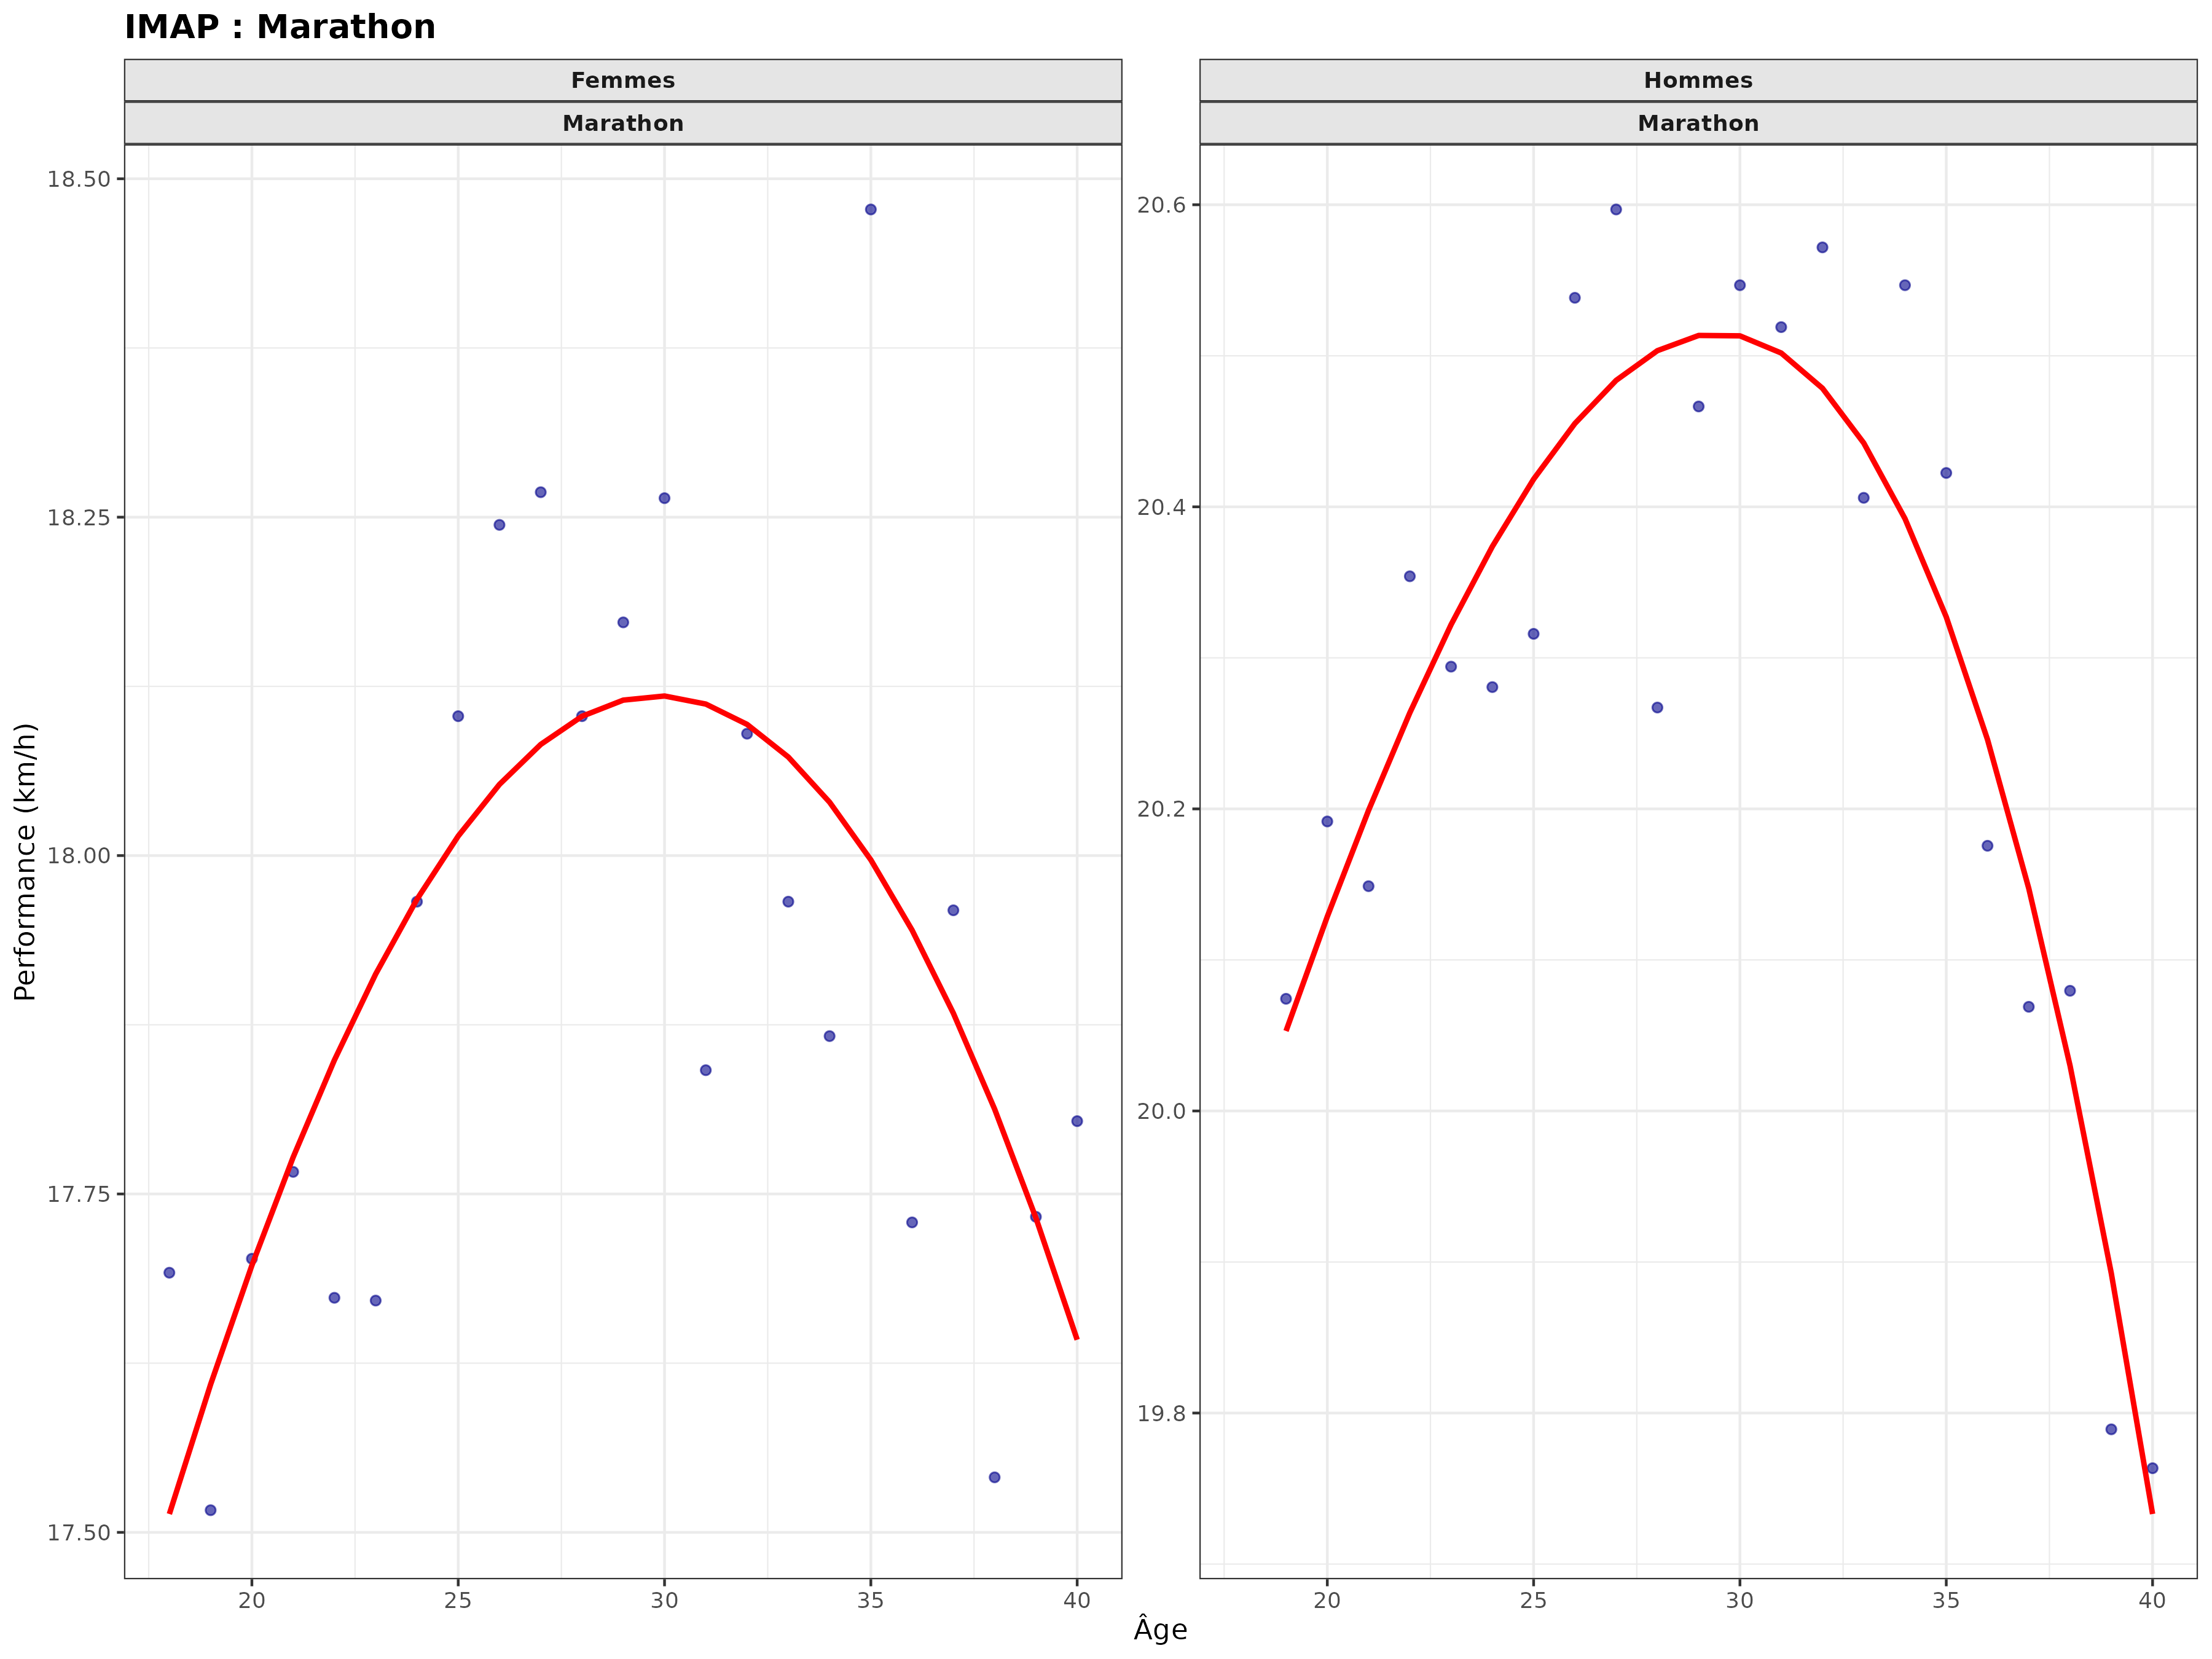
\includegraphics[width=0.9\linewidth,height=\textheight,keepaspectratio]{annexes/imap_marathon.png}

}

\caption{\label{fig-imap-marathon}Ajustement du modèle IMAP sur le
marathon (hommes et femmes). Points : meilleure performance annuelle par
âge. Ligne rouge : courbe ajustée.}

\end{figure}%

\subsubsection*{Comparaison des modèles Moore et
IMAP}\label{comparaison-des-moduxe8les-moore-et-imap}
\addcontentsline{toc}{subsubsection}{Comparaison des modèles Moore et
IMAP}

\paragraph*{Âges au pic}\label{uxe2ges-au-pic}
\addcontentsline{toc}{paragraph}{Âges au pic}

Le Tableau Table~\ref{tbl-comparatif-pic} présente les âges au pic
estimés par les deux modèles pour l'ensemble des disciplines.

\begin{longtable}[]{@{}lcccc@{}}
\caption{Âges au pic estimés (en années) par les modèles Moore et IMAP,
selon la discipline et le sexe}\label{tbl-comparatif-pic}\tabularnewline
\toprule\noalign{}
Discipline & Moore H & IMAP H & Moore F & IMAP F \\
\midrule\noalign{}
\endfirsthead
\toprule\noalign{}
Discipline & Moore H & IMAP H & Moore F & IMAP F \\
\midrule\noalign{}
\endhead
\bottomrule\noalign{}
\endlastfoot
100m & 27,6 & 29,2 & 28,1 & 28,2 \\
200m & 24,7 & 25,3 & 27,4 & 26,9 \\
400m & 25,1 & 26,6 & 25,1 & 26,8 \\
Haies hautes & 27,2 & 26,9 & 27,0 & 28,0 \\
400m haies & 25,7 & 27,0 & 26,9 & 26,4 \\
800m & 23,8 & 25,2 & 25,1 & 26,4 \\
1500m & 26,0 & 27,7 & 25,6 & 27,1 \\
3000m steeple & 26,8 & 26,8 & 25,8 & 24,9 \\
5000m & 24,0 & 25,4 & 24,4 & 25,8 \\
10 000m & 22,3 & 24,9 & 28,1 & 28,3 \\
Marathon & 29,7 & 29,5 & 29,3 & 29,8 \\
Marche & 27,2 & 28,2 & 26,1 & 27,3 \\
Longueur & 25,9 & 26,3 & 26,8 & 27,0 \\
Triple saut & 26,9 & 28,0 & 27,0 & 28,2 \\
Hauteur & 25,1 & 26,3 & 26,7 & 27,8 \\
Perche & 27,9 & 28,4 & 28,5 & 28,7 \\
Javelot & 28,5 & 26,8 & 27,5 & 27,6 \\
Disque & 30,9 & 30,0 & 28,7 & 28,3 \\
Poids & 29,9 & 28,7 & 28,7 & 27,2 \\
Marteau & 29,5 & 28,9 & 27,1 & 27,2 \\
Épreuves combinées & 27,2 & 26,6 & 27,0 & 25,3 \\
\end{longtable}

Les deux modèles produisent des estimations globalement cohérentes, avec
des écarts souvent inférieurs à 2 ans (Table~\ref{tbl-comparatif-pic}).
Les convergences les plus nettes apparaissent pour les disciplines
d'endurance longue : au marathon, l'écart entre Moore et IMAP est
inférieur à 0,5 an pour les deux sexes. Les divergences les plus
importantes concernent le sprint et le demi-fond : au 100m hommes, Moore
estime le pic à 27,6 ans contre 29,2 ans pour IMAP ; au 10 000m hommes,
l'écart est inverse avec 22,3 ans (Moore) contre 24,9 ans (IMAP). Pour
les lancers, les deux modèles s'accordent sur des pics tardifs, au-delà
de 28 ans.

\paragraph*{Qualité d'ajustement : RMSE, AIC et
BIC}\label{qualituxe9-dajustement-rmse-aic-et-bic}
\addcontentsline{toc}{paragraph}{Qualité d'ajustement : RMSE, AIC et
BIC}

Le Tableau Table~\ref{tbl-comparatif-rmse} présente les RMSE obtenus par
les deux modèles. Les erreurs résiduelles sont proches entre les deux
modèles. IMAP présente un RMSE inférieur sur plusieurs disciplines : au
marteau hommes (1,319 contre 1,986, soit −34 \%), au poids femmes (0,226
contre 0,446, soit −49 \%), et au 10 000m hommes (0,277 contre 0,550).
Moore présente en revanche un RMSE légèrement inférieur sur plusieurs
disciplines de course courte et de demi-fond.

\begin{longtable}[]{@{}lcccc@{}}
\caption{RMSE par modèle, discipline et
sexe}\label{tbl-comparatif-rmse}\tabularnewline
\toprule\noalign{}
Discipline & RMSE Moore H & RMSE IMAP H & RMSE Moore F & RMSE IMAP F \\
\midrule\noalign{}
\endfirsthead
\toprule\noalign{}
Discipline & RMSE Moore H & RMSE IMAP H & RMSE Moore F & RMSE IMAP F \\
\midrule\noalign{}
\endhead
\bottomrule\noalign{}
\endlastfoot
100m & 0,324 & 0,443 & 0,264 & 0,257 \\
200m & 0,683 & 0,683 & 0,311 & 0,427 \\
400m & 0,350 & 0,395 & 0,327 & 0,413 \\
Haies hautes & 0,370 & 0,363 & 0,388 & 0,428 \\
400m haies & 0,084 & 0,094 & 0,053 & 0,063 \\
800m & 0,282 & 0,342 & 0,407 & 0,447 \\
1500m & 0,194 & 0,238 & 0,319 & 0,346 \\
3000m steeple & 0,214 & 0,234 & 0,397 & 0,412 \\
5000m & 0,148 & 0,176 & 0,205 & 0,234 \\
10 000m & 0,550 & 0,277 & 0,480 & 0,507 \\
Marathon & 0,129 & 0,101 & 0,201 & 0,196 \\
Marche & 0,002 & 0,002 & 0,001 & 0,001 \\
Longueur & 0,171 & 0,178 & 0,149 & 0,150 \\
Triple saut & 0,171 & 0,190 & 0,195 & 0,198 \\
Hauteur & 0,037 & 0,040 & 0,019 & 0,020 \\
Perche & 0,096 & 0,099 & 0,008 & 0,082 \\
Javelot & 3,083 & 2,875 & 1,550 & 1,515 \\
Disque & 1,726 & 1,663 & 1,697 & 1,714 \\
Poids & 0,501 & 0,419 & 0,446 & 0,226 \\
Marteau & 1,986 & 1,319 & 1,156 & 1,174 \\
Épreuves combinées & 147,9 & 134,6 & 174,9 & 138,9 \\
\end{longtable}

La comparaison des critères AIC et BIC confirme cette absence de
dominance systématique : IMAP obtient de meilleurs critères sur le
marathon hommes, le 10 000m hommes et les épreuves combinées ; Moore
obtient de meilleurs critères sur la majorité des disciplines de course
courte et de demi-fond.

\begin{longtable}[]{@{}lcccc@{}}
\caption{Critères AIC par modèle, discipline et
sexe}\label{tbl-comparatif-aic}\tabularnewline
\toprule\noalign{}
Discipline & AIC Moore H & AIC IMAP H & AIC Moore F & AIC IMAP F \\
\midrule\noalign{}
\endfirsthead
\toprule\noalign{}
Discipline & AIC Moore H & AIC IMAP H & AIC Moore F & AIC IMAP F \\
\midrule\noalign{}
\endhead
\bottomrule\noalign{}
\endlastfoot
100m & 20,2 & 35,8 & 6,4 & 8,6 \\
200m & 55,5 & 55,4 & 17,7 & 32,9 \\
400m & 23,3 & 29,2 & 19,5 & 31,3 \\
Haies hautes & 24,3 & 24,3 & 28,3 & 33,0 \\
400m haies & -43,0 & -38,1 & - 58,4 & - 51,0 \\
800m & 12,0 & 20,1 & 31,7 & 36,4 \\
1500m & - 5,1 & 4,8 & 19,5 & 23,5 \\
3000m steeple & 0,0 & 4,0 & 27,4 & 29,0 \\
5000m & - 18,0 & - 9,7 & - 2,4 & 4,0 \\
10 000m & 43,4 & 11,7 & 37,1 & 39,6 \\
Marathon & - 20,8 & - 33,0 & - 2,9 & - 4,0 \\
Marche & - 230,8 & - 229,8 & - 258,3 & - 252,1 \\
Longueur & - 10,3 & - 8,6 & - 17,7 & - 17,3 \\
Triple saut & - 11,7 & - 6,3 & - 5,1 & - 4,5 \\
Hauteur & - 87,7 & - 84,9 & - 121,8 & - 118,7 \\
Perche & - 40,6 & - 38,9 & - 48,8 & - 48,6 \\
Javelot & 132,9 & 129,4 & 98,5 & 97,4 \\
Disque & 103,9 & 102,0 & 103,0 & 103,5 \\
Poids & 40,6 & 32,0 & 36,2 & 2,3 \\
Marteau & 110,9 & 90,4 & 83,8 & 84,6 \\
Épreuves combinées & 275,0 & 271,1 & 308,4 & 297,9 \\
\end{longtable}

\begin{longtable}[]{@{}lcccc@{}}
\caption{Critères BIC par modèle, discipline et
sexe}\label{tbl-comparatif-bic}\tabularnewline
\toprule\noalign{}
Discipline & BIC Moore H & BIC IMAP H & BIC Moore F & BIC IMAP F \\
\midrule\noalign{}
\endfirsthead
\toprule\noalign{}
Discipline & BIC Moore H & BIC IMAP H & BIC Moore F & BIC IMAP F \\
\midrule\noalign{}
\endhead
\bottomrule\noalign{}
\endlastfoot
100m & 26,3 & 41,9 & 12,3 & 14,4 \\
200m & 61,4 & 61,3 & 23,6 & 38,8 \\
400m & 29,2 & 35,1 & 25,2 & 37,2 \\
Haies hautes & 29,7 & 30,0 & 34,2 & 38,9 \\
400m haies & - 37,3 & - 32,4 & -53,2 & -45,7 \\
800m & 17,2 & 25,3 & 37,8 & 42,5 \\
1500m & 0,8 & 10,7 & 25,6 & 29,5 \\
3000m steeple & 5,7 & 9,7 & 32,8 & 34,4 \\
5000m & -12,1 & -3,8 & 3,5 & 9,9 \\
10 000m & 49,1 & 17,4 & 42,8 & 45,3 \\
Marathon & -15,6 & -27,6 & 2,8 & 1,6 \\
Marche & -224,9 & -223,9 & -252,2 & -246,0 \\
Longueur & -4,6 & -2,9 & -11,8 & -11,4 \\
Triple saut & -5,6 & -0,3 & 1,0 & 1,6 \\
Hauteur & -81,6 & -78,8 & -115,7 & -112,6 \\
Perche & -34,5 & -32,8 & -42,7 & -42,5 \\
Javelot & 139,0 & 135,5 & 104,6 & 103,5 \\
Disque & 110,0 & 108,1 & 109,1 & 109,6 \\
Poids & 46,5 & 38,0 & 42,3 & 8,4 \\
Marteau & 117,0 & 96,5 & 89,9 & 90,7 \\
Épreuves combinées & 280,2 & 276,3 & 314,1 & 303,5 \\
\end{longtable}

\subsection{Discussion}\label{discussion-2}

\subsubsection{Âge au pic selon la famille de
disciplines}\label{uxe2ge-au-pic-selon-la-famille-de-disciplines}

Les résultats confirment l'hypothèse d'une variabilité de l'âge au pic
selon la filière énergétique sollicitée, conformément aux travaux
d'Allen et Hopkins (\citeproc{ref-Allen2015}{Allen et Hopkins 2015}). Le
pic plus tardif observé dans les lancers (28--30 ans) s'explique par la
dépendance de ces disciplines à la force maximale, qui atteint son
apogée plus tardivement que la vitesse explosive
(\citeproc{ref-Komi1992}{Komi 1992}). À l'inverse, la précocité relative
des épreuves de sprint et de demi-fond peut être associée à la
prédominance des fibres musculaires rapides et à la capacité anaérobie,
qualités qui culminent plus tôt dans la vie adulte
(\citeproc{ref-Tanaka2003}{Tanaka et Seals 2003}). Le marathon constitue
un cas particulier : le pic tardif estimé à près de 30 ans pour les deux
sexes est cohérent avec la littérature sur l'endurance longue, qui
souligne le rôle déterminant de l'expérience de course accumulée et de
la maturité physiologique aérobie (\citeproc{ref-Allen2015}{Allen et
Hopkins 2015}).

\subsubsection{Différences entre
sexes}\label{diffuxe9rences-entre-sexes}

Les écarts observés entre hommes et femmes restent faibles (1 à 2 ans au
maximum) et non systématiques selon les disciplines, ce qui est cohérent
avec les conclusions d'Allen et Hopkins (\citeproc{ref-Allen2015}{Allen
et Hopkins 2015}). Ces différences pourraient partiellement s'expliquer
par des trajectoires de développement hormonal distinctes : la
testostérone, dont le pic survient plus tôt chez les hommes, favorise un
gain de masse musculaire et de puissance explosive précoce, tandis que
les adaptations physiologiques féminines, notamment cardiovasculaires,
se développeraient sur une fenêtre temporelle légèrement plus étendue
(\citeproc{ref-Deaner2012}{Deaner, Lowen, et Cobley 2012}). Toutefois,
la faiblesse des écarts invite à nuancer l'influence du sexe comme
facteur déterminant de l'âge au pic en athlétisme d'élite.

\subsubsection{Comparaison des modèles Moore et
IMAP}\label{comparaison-des-moduxe8les-moore-et-imap-1}

L'absence de dominance systématique d'un modèle sur l'autre suggère que
les deux formulations capturent des dynamiques similaires sur la fenêtre
d'observation restreinte (16--40 ans). Les divergences les plus marquées
dans les disciplines de sprint et de demi-fond pourraient s'expliquer
par la sensibilité respective des deux modèles aux optima locaux sur des
données peu étendues aux âges extrêmes. La richesse interprétative du
modèle IMAP, dont les paramètres sont ancrés dans une théorie biologique
cellulaire (\citeproc{ref-Berthelot2019}{Berthelot et al. 2012}),
constitue un argument en sa faveur indépendamment des seuls critères
statistiques, notamment pour des usages prospectifs ou comparatifs entre
populations. \newpage

\section{Discussion générale}\label{discussion-guxe9nuxe9rale}

\newpage

\section*{Conclusion}\label{conclusion}
\addcontentsline{toc}{section}{Conclusion}

\newpage

\section*{Remerciements}\label{remerciements}
\addcontentsline{toc}{section}{Remerciements}

\newpage

\section*{Références}\label{ruxe9fuxe9rences}
\addcontentsline{toc}{section}{Références}

Voici la liste de toutes les références bibliographiques utiles à la
rédaction de ce rapport :

\phantomsection\label{refs}
\begin{CSLReferences}{1}{0}
\bibitem[\citeproctext]{ref-Allen2015}
Allen, Scott V., et William G. Hopkins. 2015. {«~Age of Peak Competitive
Performance of Elite Athletes: A Systematic Review~»}. \emph{Sports
Medicine} 45 (10): 1431‑41.
\url{https://doi.org/10.1007/s40279-015-0354-3}.

\bibitem[\citeproctext]{ref-Berthelot2019}
Berthelot, Geoffroy, Sylvain Len, Philippe Hellard, Muriel Tafflet,
Marion Guillaume, Jean-Claude Vollmer, Bruno Gager, Laurent Quinquis,
Andy Marc, et Jean-François Toussaint. 2012. {«~Exponential Growth
Combined with Exponential Decline Explains Lifetime Performance
Evolution in Individual and Human Species~»}. \emph{Age} 34 (4): 1001‑9.
\url{https://doi.org/10.1007/s11357-011-9274-9}.

\bibitem[\citeproctext]{ref-Carter2019}
Carter, P. A. et al. s.~d. {«~The age-performance relationship in the
general population and strategies to delay age related decline in
performance~»}. \emph{Archives of Public Health}.
\url{https://doi.org/10.1186/s13690-019-0375-8}.

\bibitem[\citeproctext]{ref-Deaner2012}
Deaner, Robert O., Alyssa Lowen, et Steve Cobley. 2012. {«~Sex
Differences in Sport: Women Are Underrepresented Among the Best
Performers in Endurance Events~»}. \emph{PLOS ONE} 7 (10): e45628.
\url{https://doi.org/10.1371/journal.pone.0045628}.

\bibitem[\citeproctext]{ref-Infographic2020}
InfographicSite. 2021. {«~Olympians Age Distribution by Gender - Tokyo
2020~»}. 2021.
\url{https://infographicsite.com/infographic/olympians-age-distribution-by-gender/}.

\bibitem[\citeproctext]{ref-Komi1992}
Komi, Paavo V. 1992. \emph{Strength and Power in Sport}. Oxford:
Blackwell Scientific Publications.

\bibitem[\citeproctext]{ref-Tanaka2003}
Tanaka, Hirofumi, et Douglas R. Seals. 2003. {«~Invited Review: Dynamic
Exercise Performance in Masters Athletes: Insight into the Effects of
Primary Human Aging on Physiological Functional Capacity~»}.
\emph{Journal of Applied Physiology} 95 (5): 2152‑62.
\url{https://doi.org/10.1152/japplphysiol.00320.2003}.

\end{CSLReferences}

\newpage

\section*{Annexes}\label{annexes}
\addcontentsline{toc}{section}{Annexes}

\subsection{Compléments de l'analyse de
distribution}\label{compluxe9ments-de-lanalyse-de-distribution}

Cette section regroupe les graphiques de diagnostic complémentaires
permettant de valider les choix statistiques effectués dans le corps du
rapport.

\subsubsection{Distributions des athlètes
féminines}\label{distributions-des-athluxe8tes-fuxe9minines}

La figure ci-dessous complète l'analyse descriptive en présentant les
histogrammes de l'âge au pic pour les femmes.

\begin{figure}

\centering{

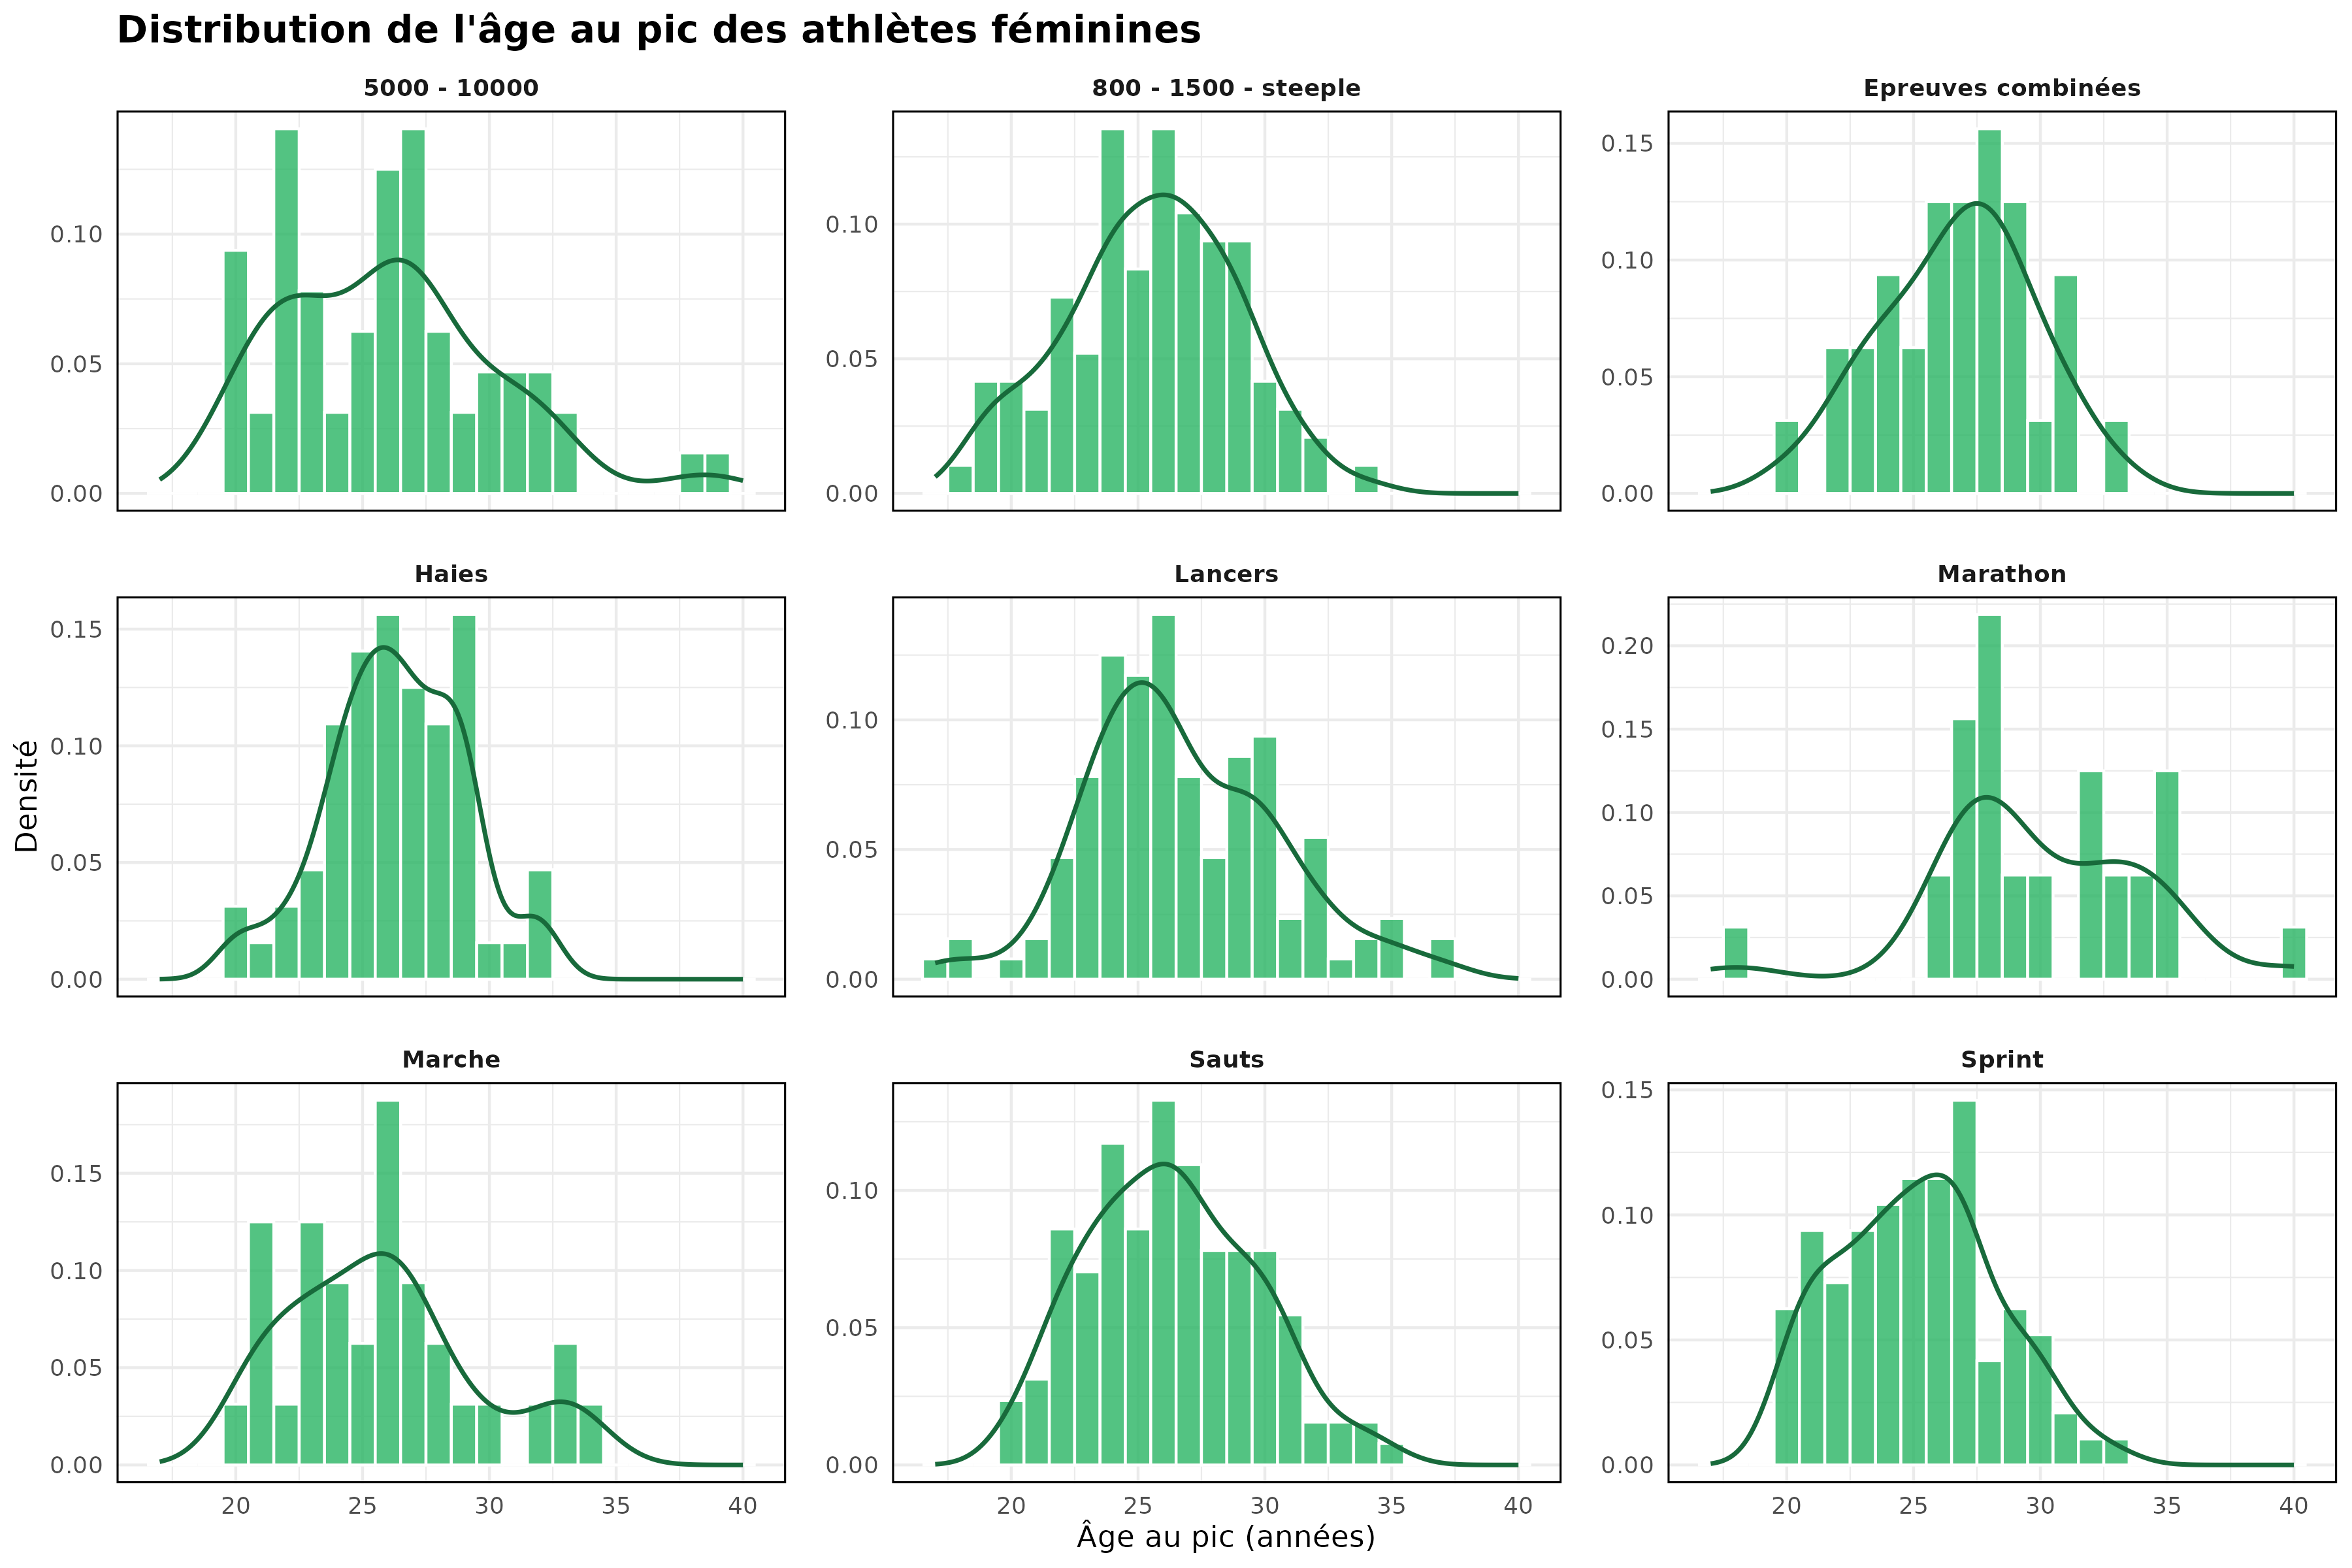
\includegraphics[width=1\linewidth,height=\textheight,keepaspectratio]{outputs/hist_age_femmes.png}

}

\caption{\label{fig-hist-women}Distributions de l'âge au pic de
performance (Athlètes féminines)}

\end{figure}%

\begin{center}\rule{0.5\linewidth}{0.5pt}\end{center}

\subsubsection{Analyse de la normalité
(QQ-Plots)}\label{analyse-de-la-normalituxe9-qq-plots}

Les graphiques Quantile-Quantile (QQ-plots) permettent de visualiser
l'écart entre nos données observées et une distribution normale
théorique (représentée par la ligne droite). Un écart des points par
rapport à cette ligne confirme la non-normalité.

\begin{figure}

\begin{minipage}{\linewidth}

\begin{figure}[H]

\centering{

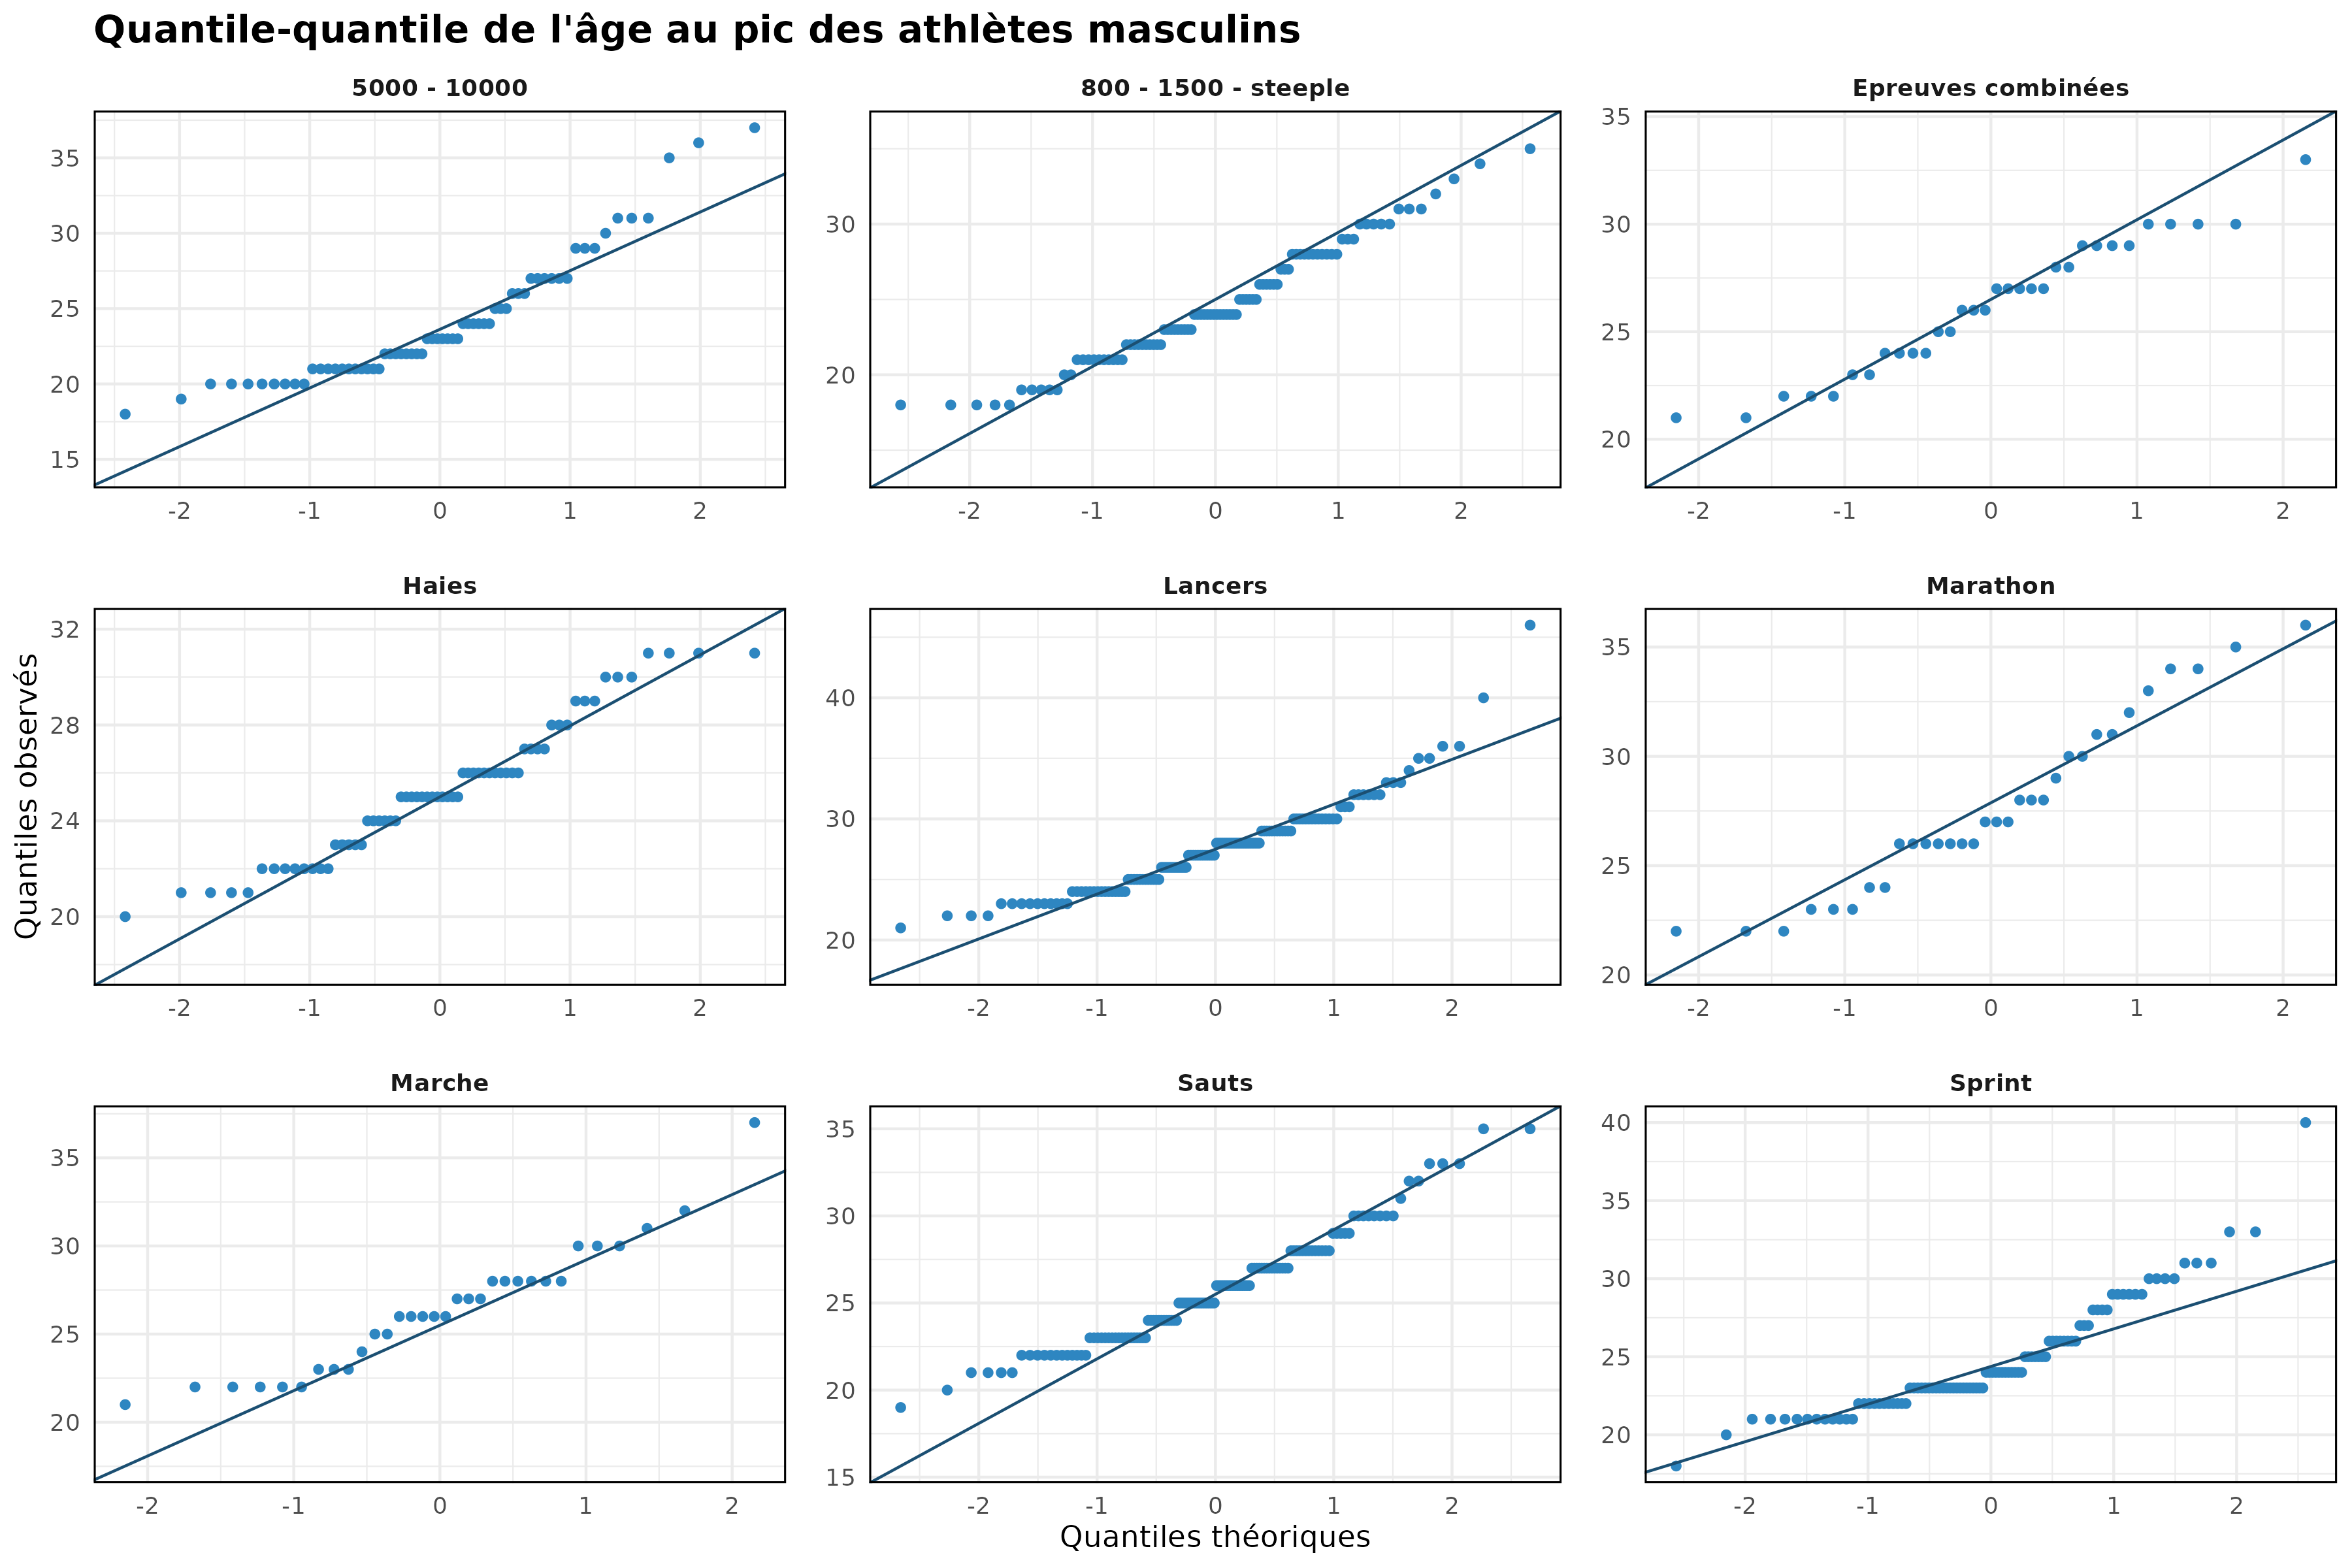
\includegraphics[width=1\linewidth,height=\textheight,keepaspectratio]{outputs/qqplot_age_hommes.png}

}

\caption{\label{fig-qq-men}QQ-plot de l'âge au pic (Hommes)}

\end{figure}%

\end{minipage}%
\newline
\begin{minipage}{\linewidth}

\begin{figure}[H]

\centering{

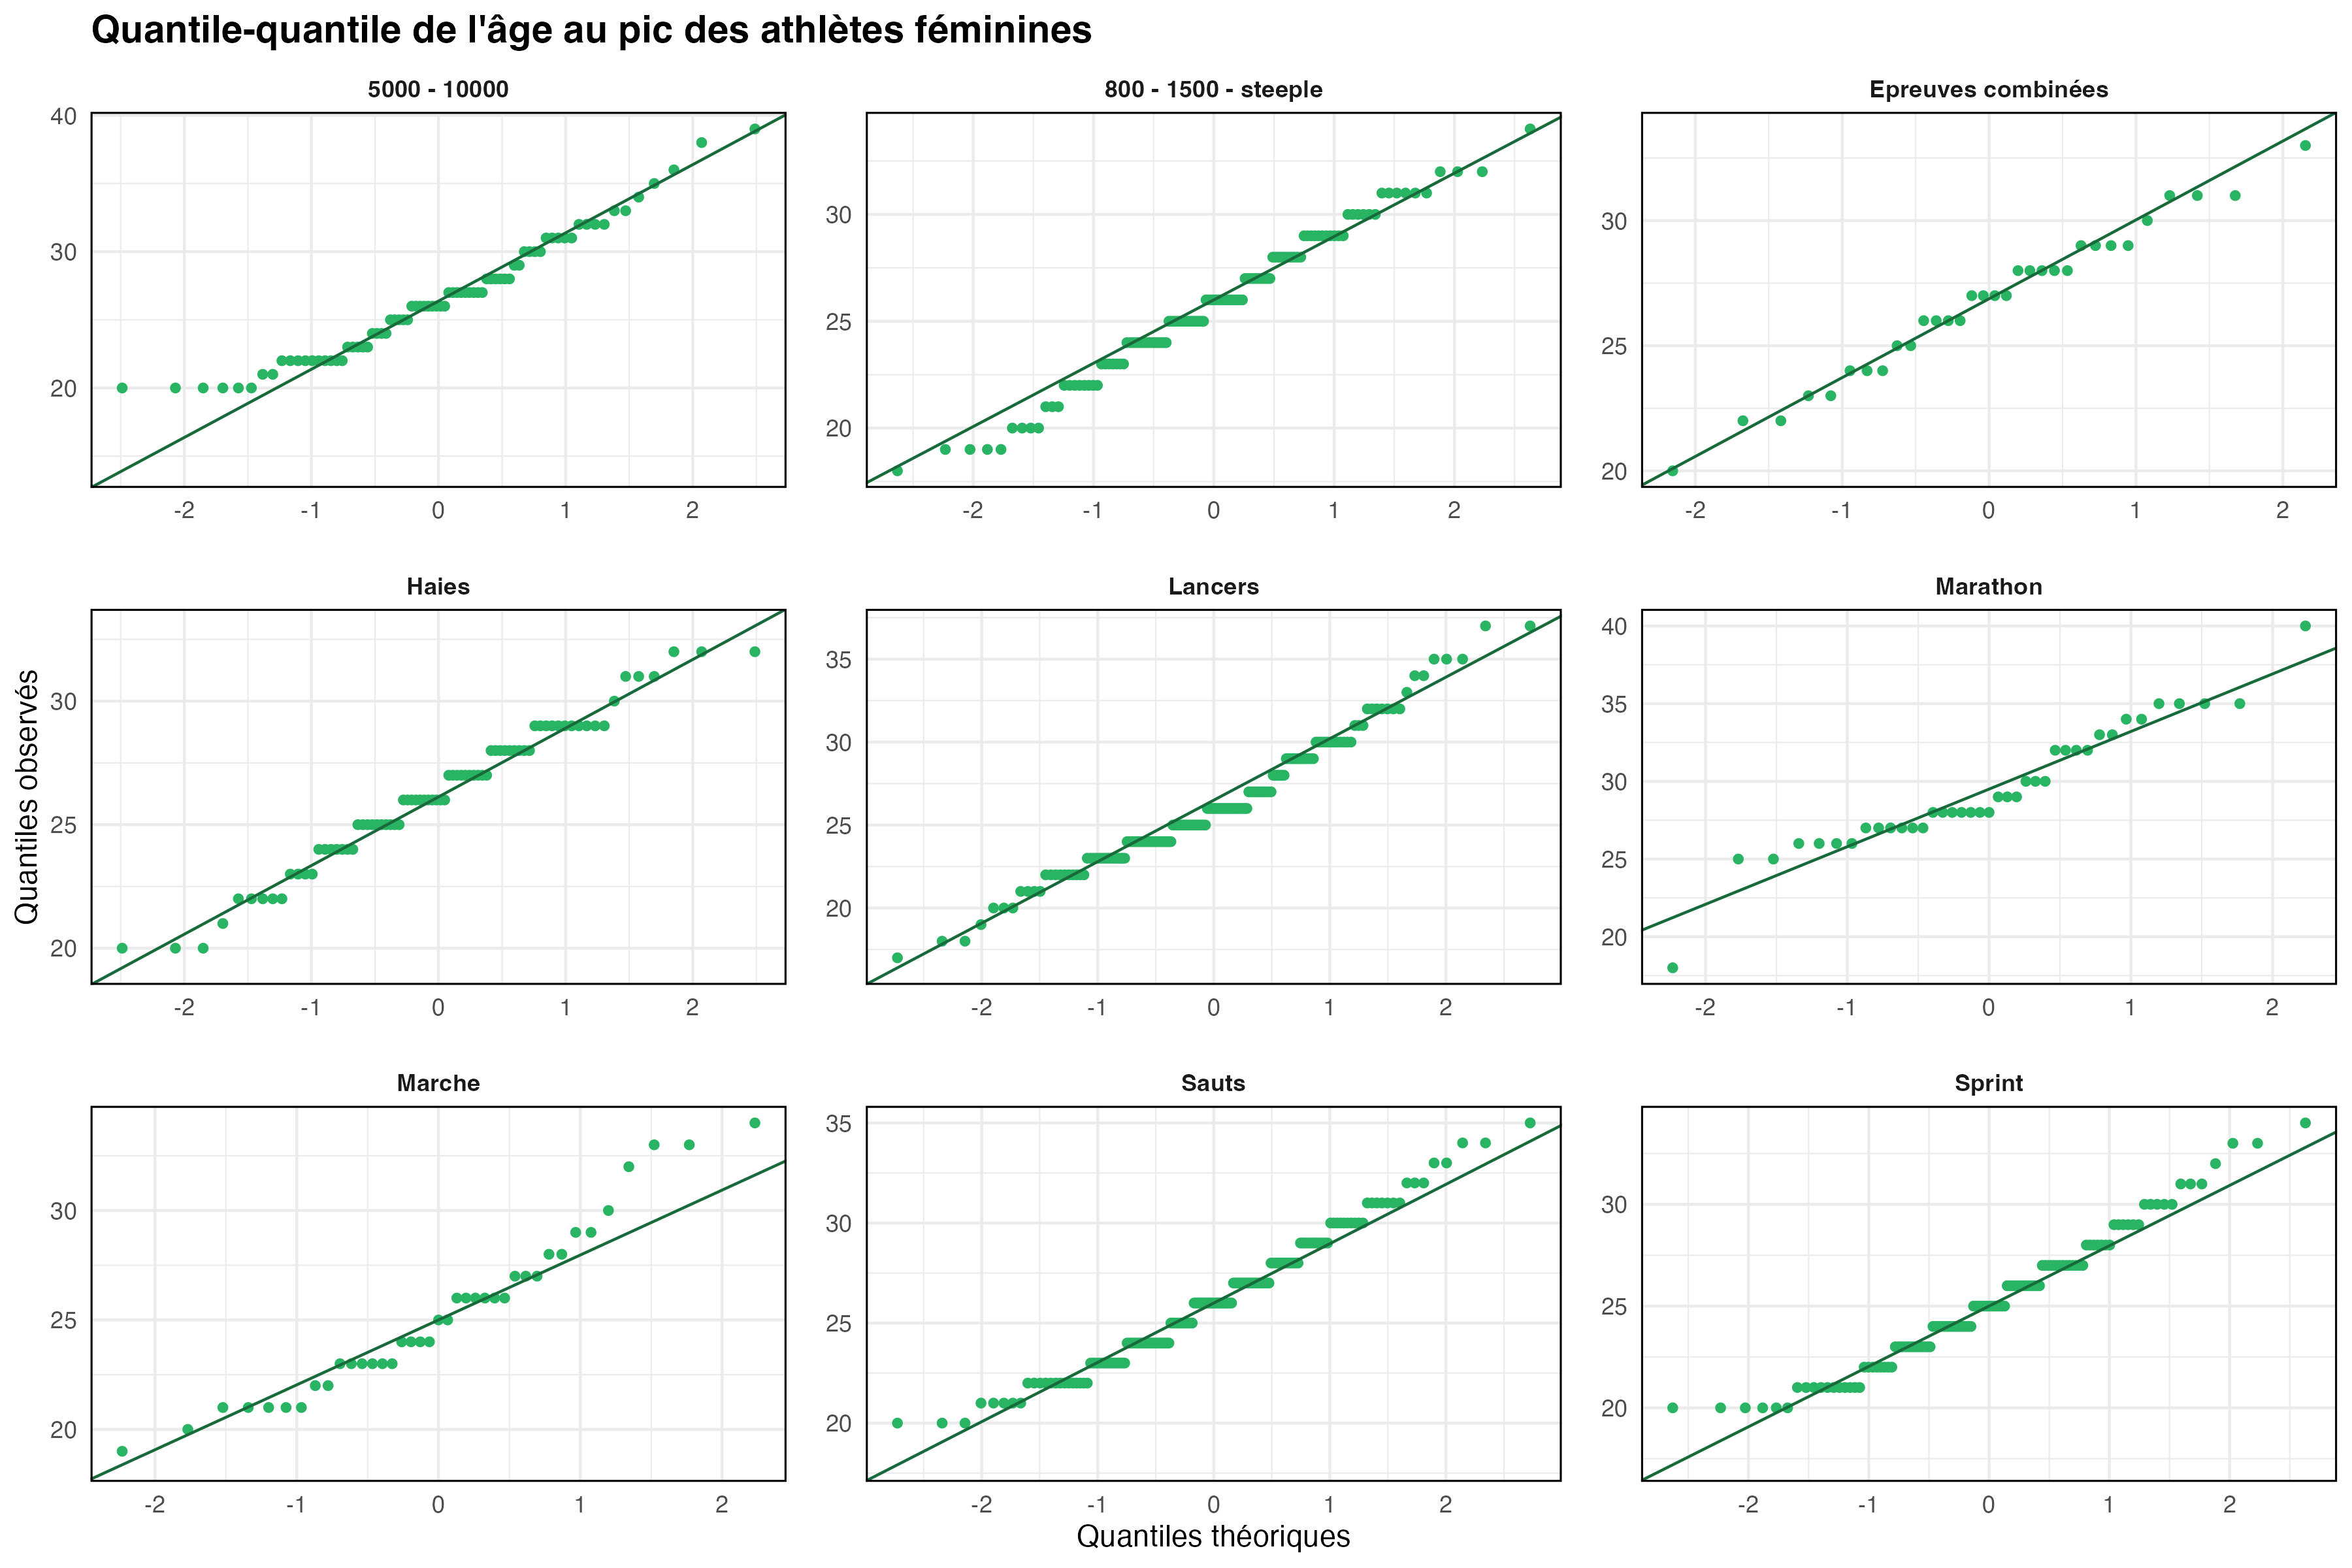
\includegraphics[width=1\linewidth,height=\textheight,keepaspectratio]{outputs/qqplot_age_femmes.png}

}

\caption{\label{fig-qq-women}QQ-plot de l'âge au pic (Femmes)}

\end{figure}%

\end{minipage}%

\end{figure}%

======= \#\# Annexe : Modèles de Moore

\begin{figure}[H]

{\centering 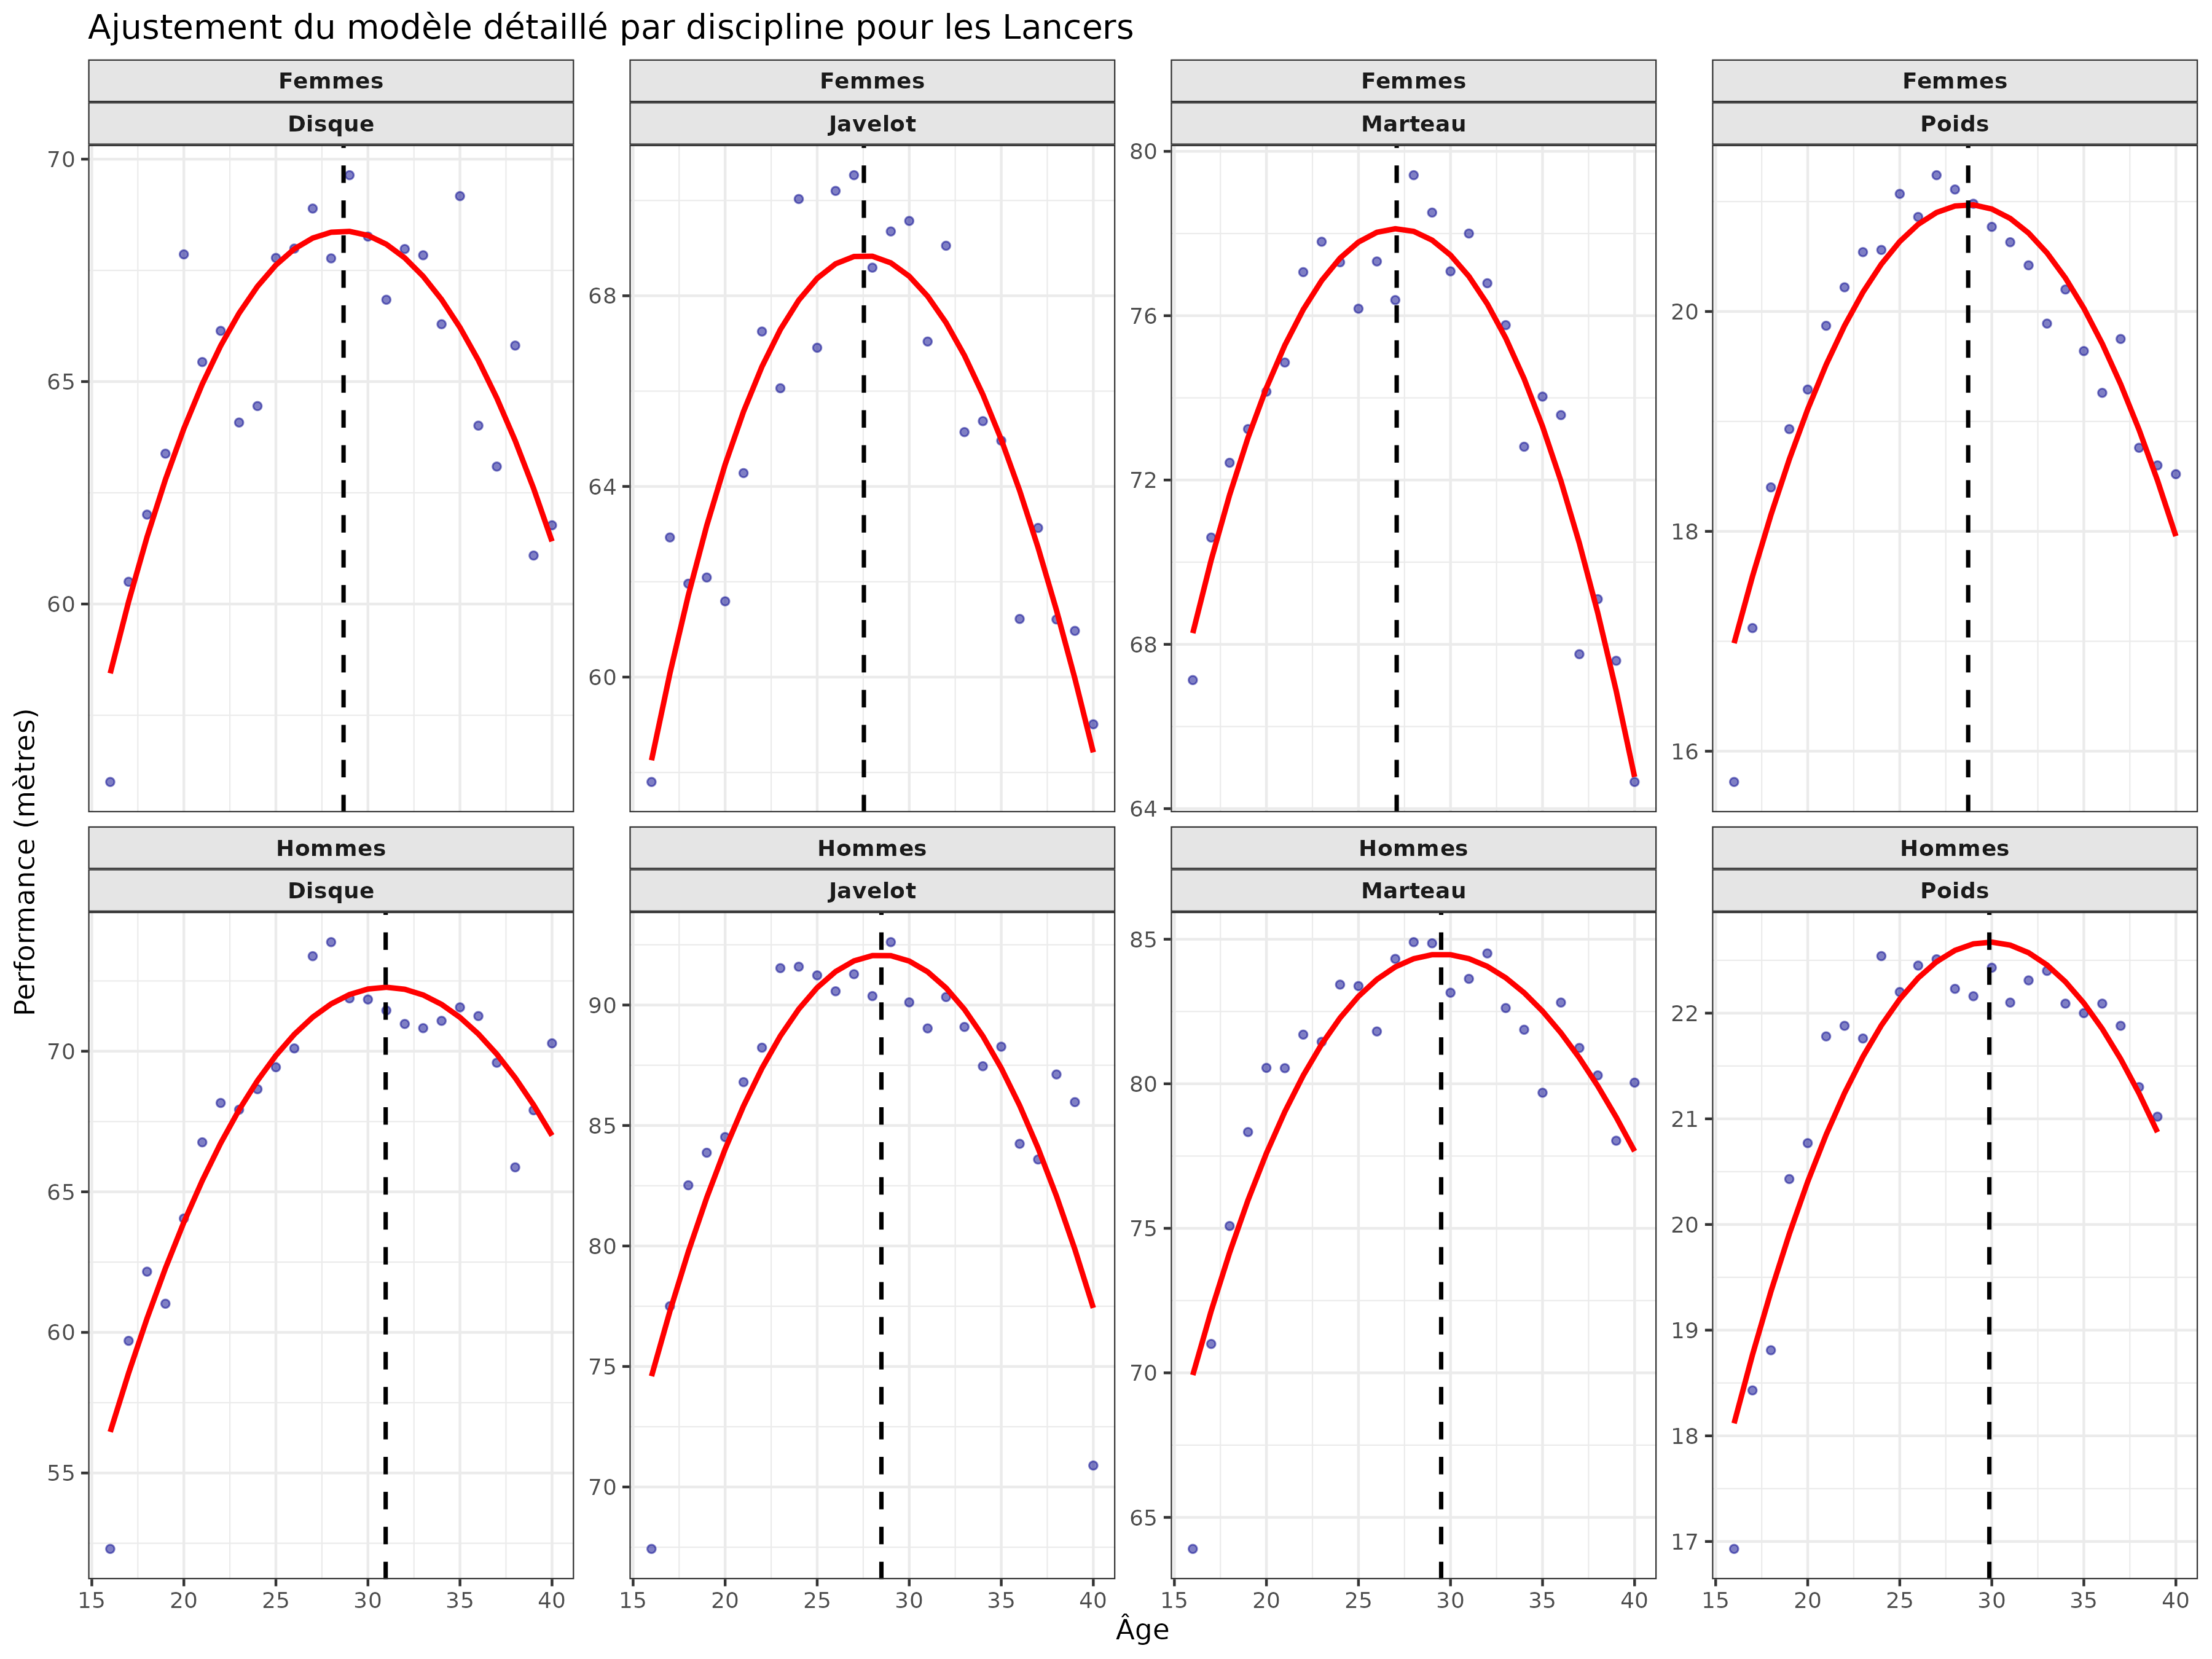
\includegraphics[width=0.8\linewidth,height=\textheight,keepaspectratio]{annexes/ajustement_lancer.png}

}

\caption{Lancers}

\end{figure}%

\begin{figure}[H]

{\centering 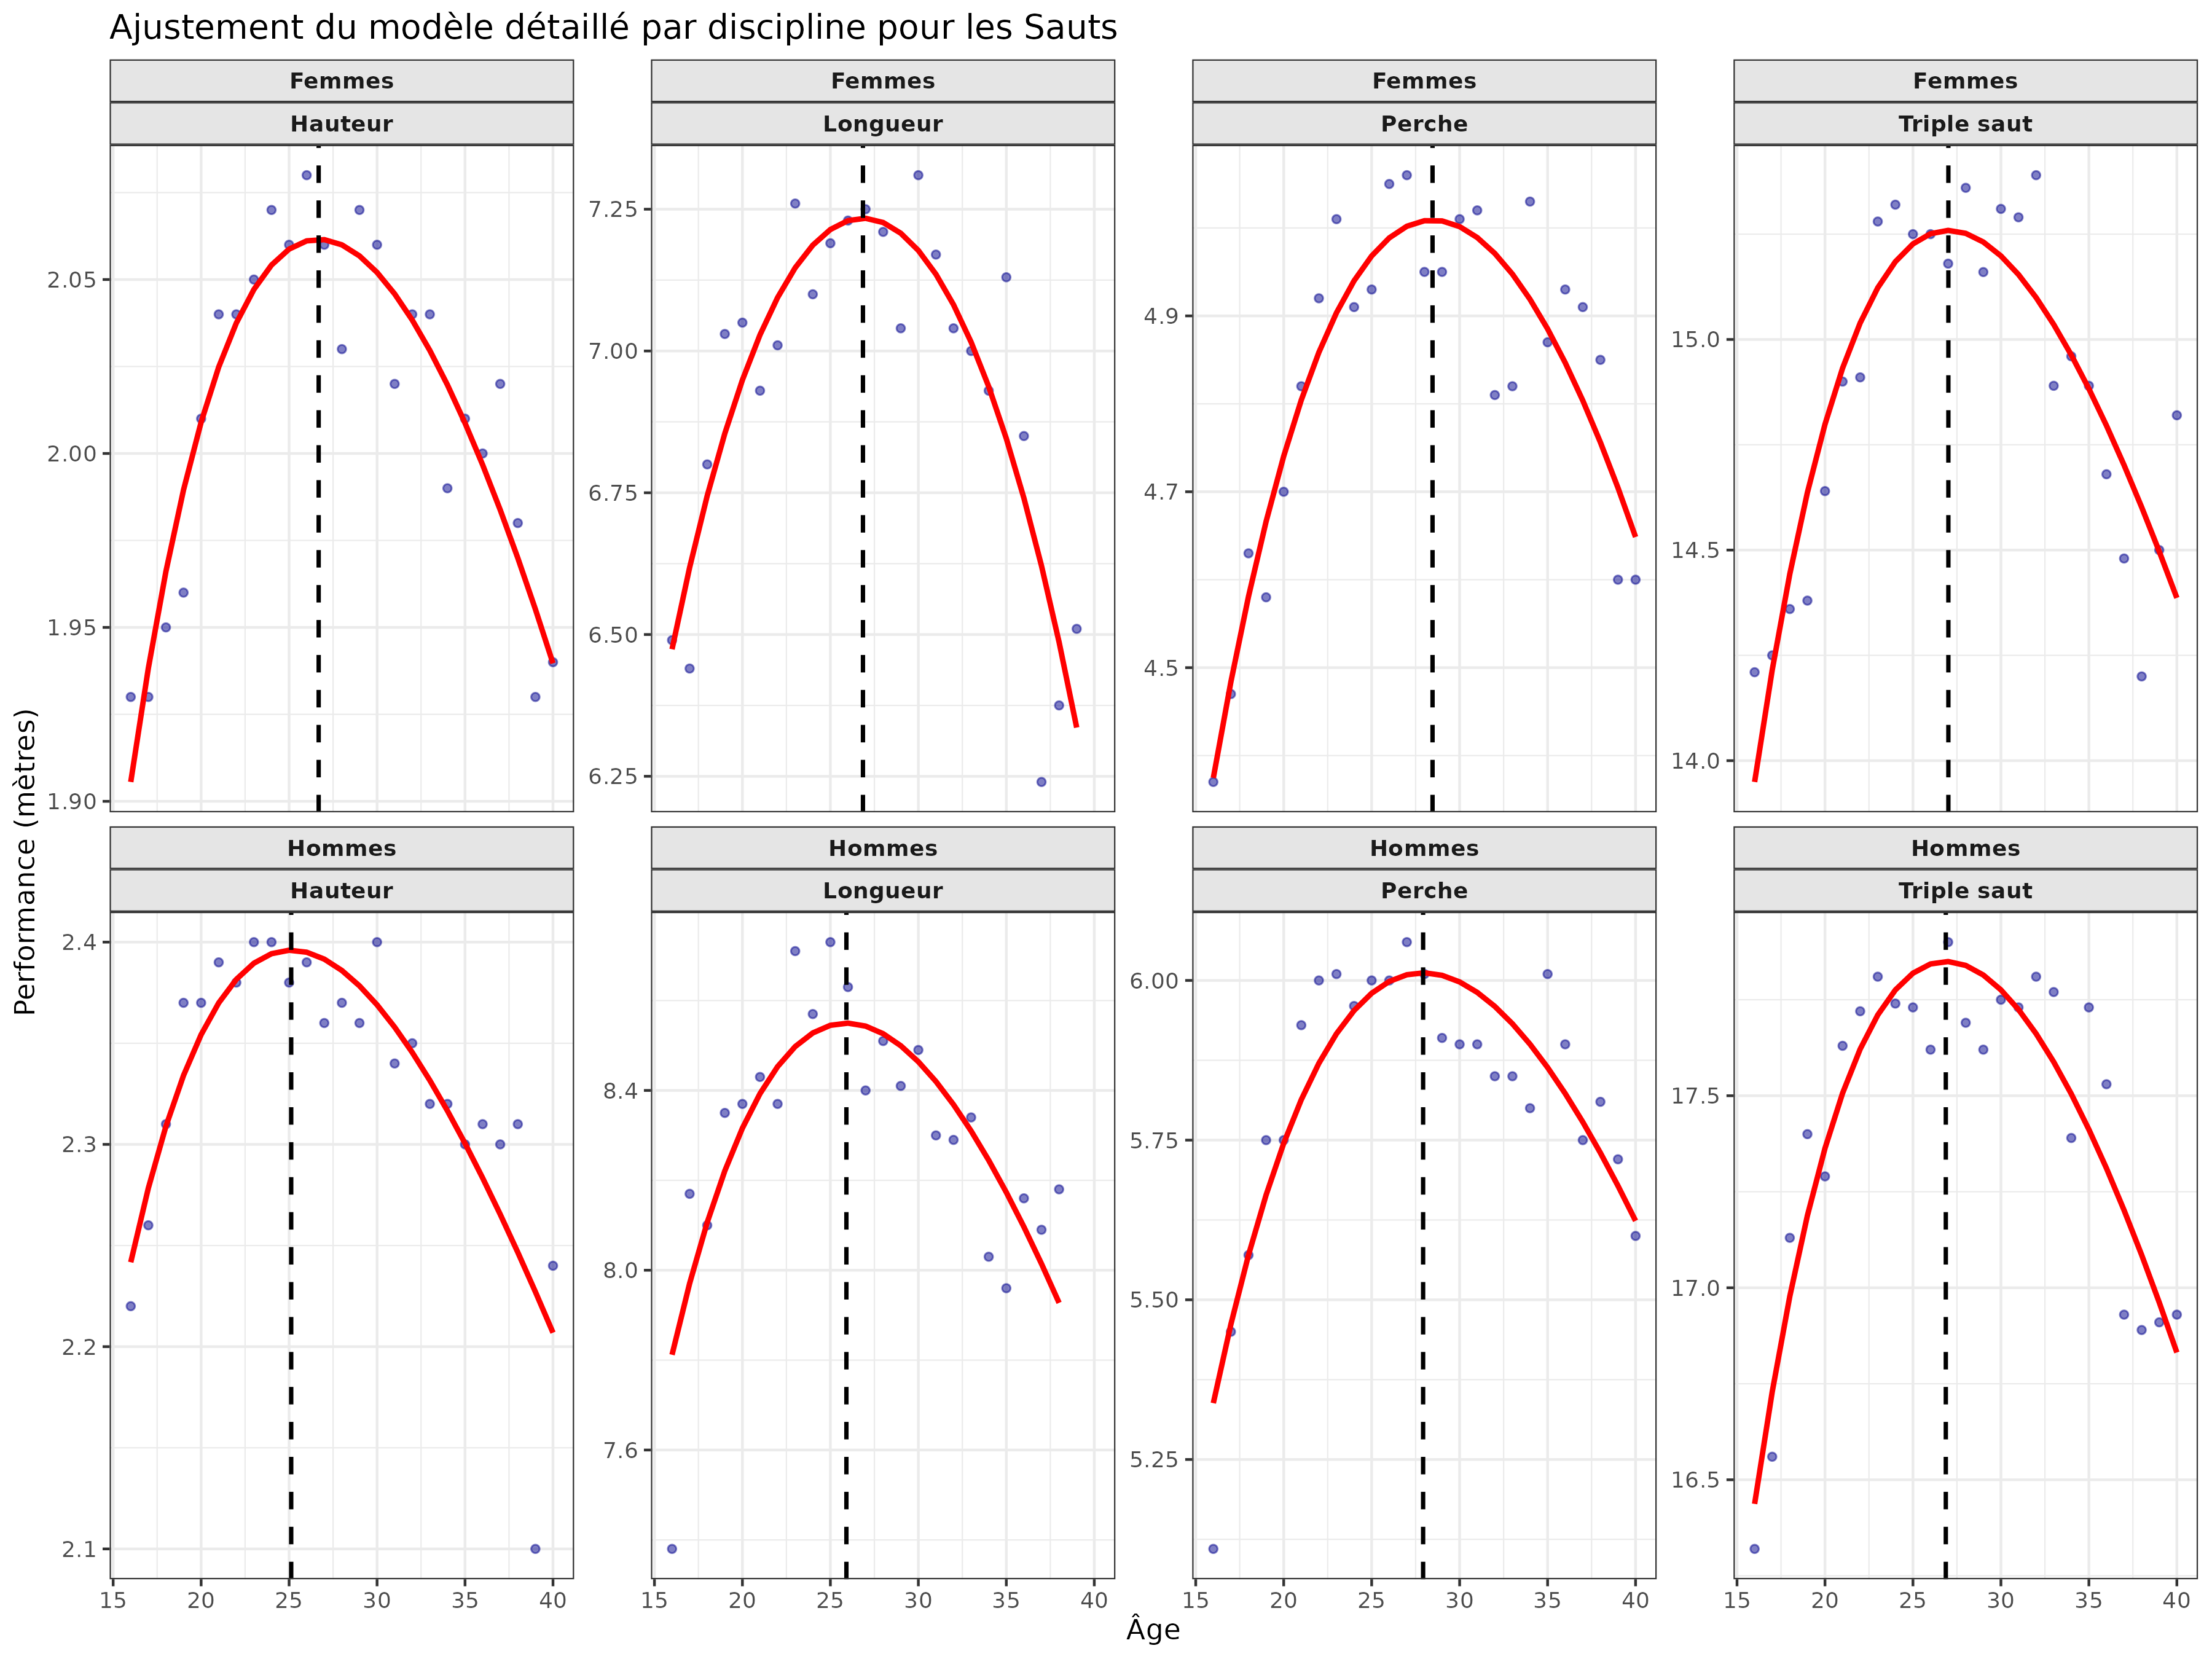
\includegraphics[width=0.8\linewidth,height=\textheight,keepaspectratio]{annexes/ajustement_saut.png}

}

\caption{Sauts}

\end{figure}%

\begin{figure}[H]

{\centering 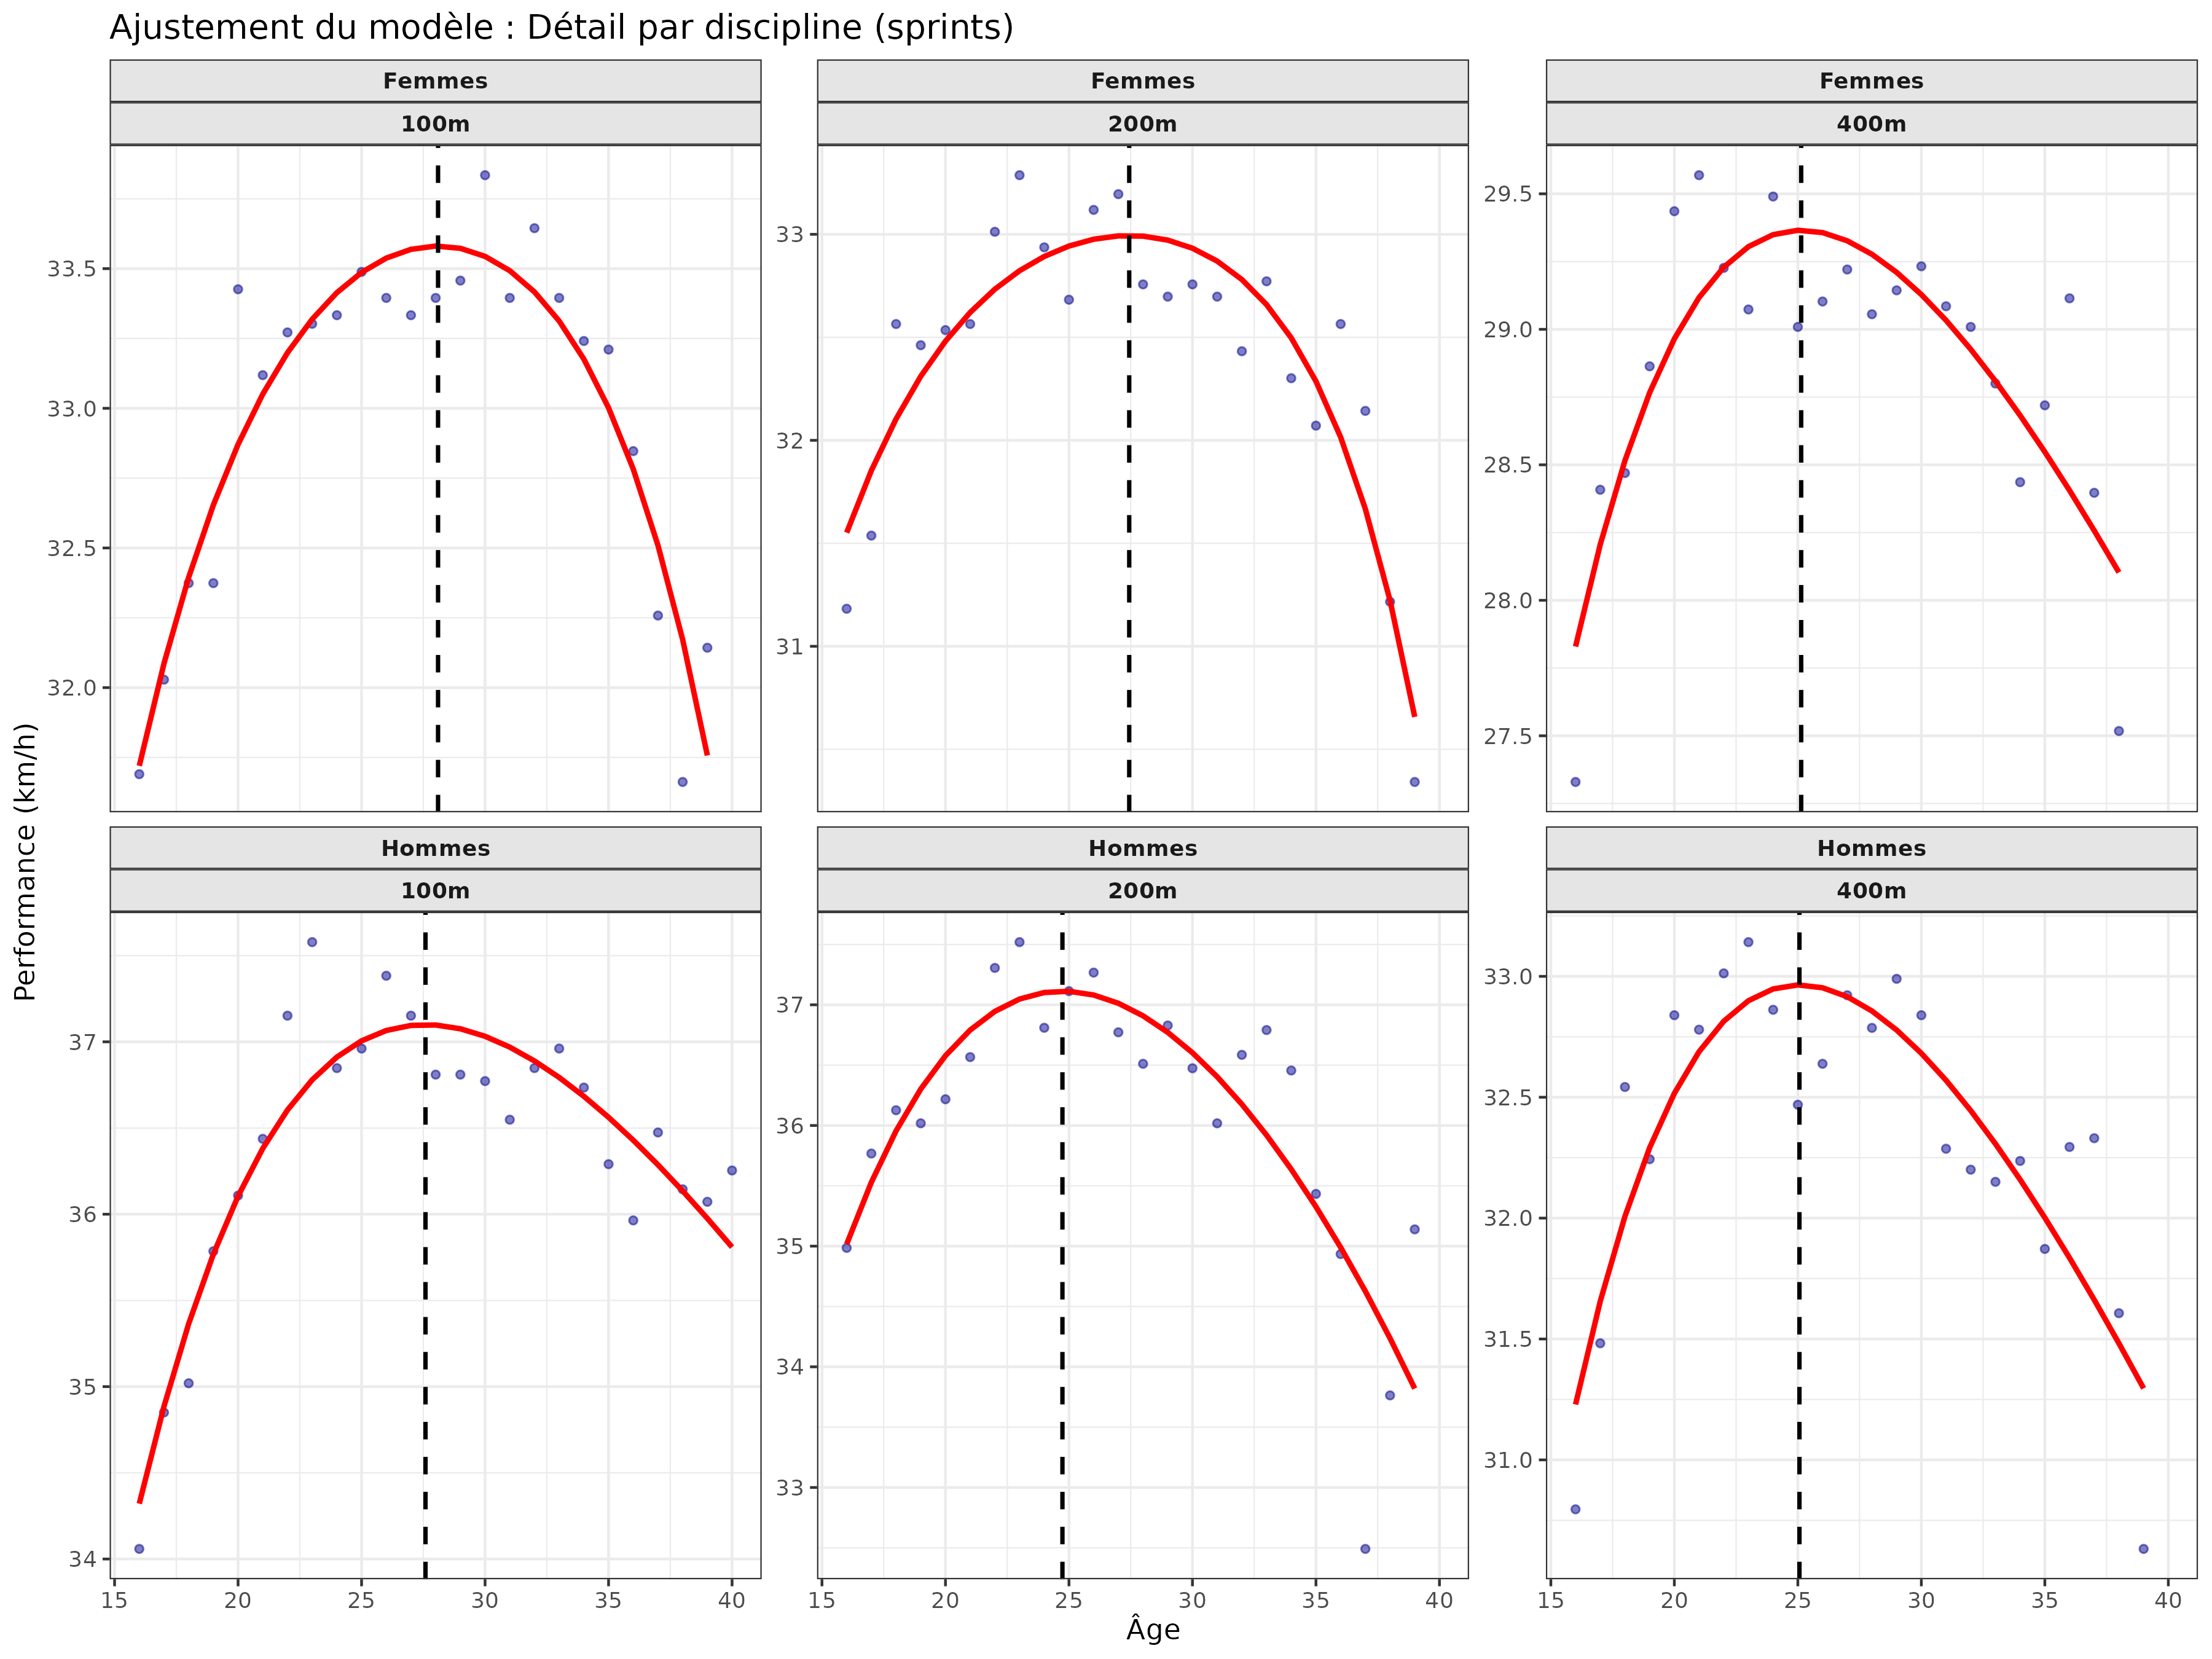
\includegraphics[width=0.8\linewidth,height=\textheight,keepaspectratio]{annexes/ajustement_sprint.png}

}

\caption{Sprint}

\end{figure}%

\begin{figure}[H]

{\centering 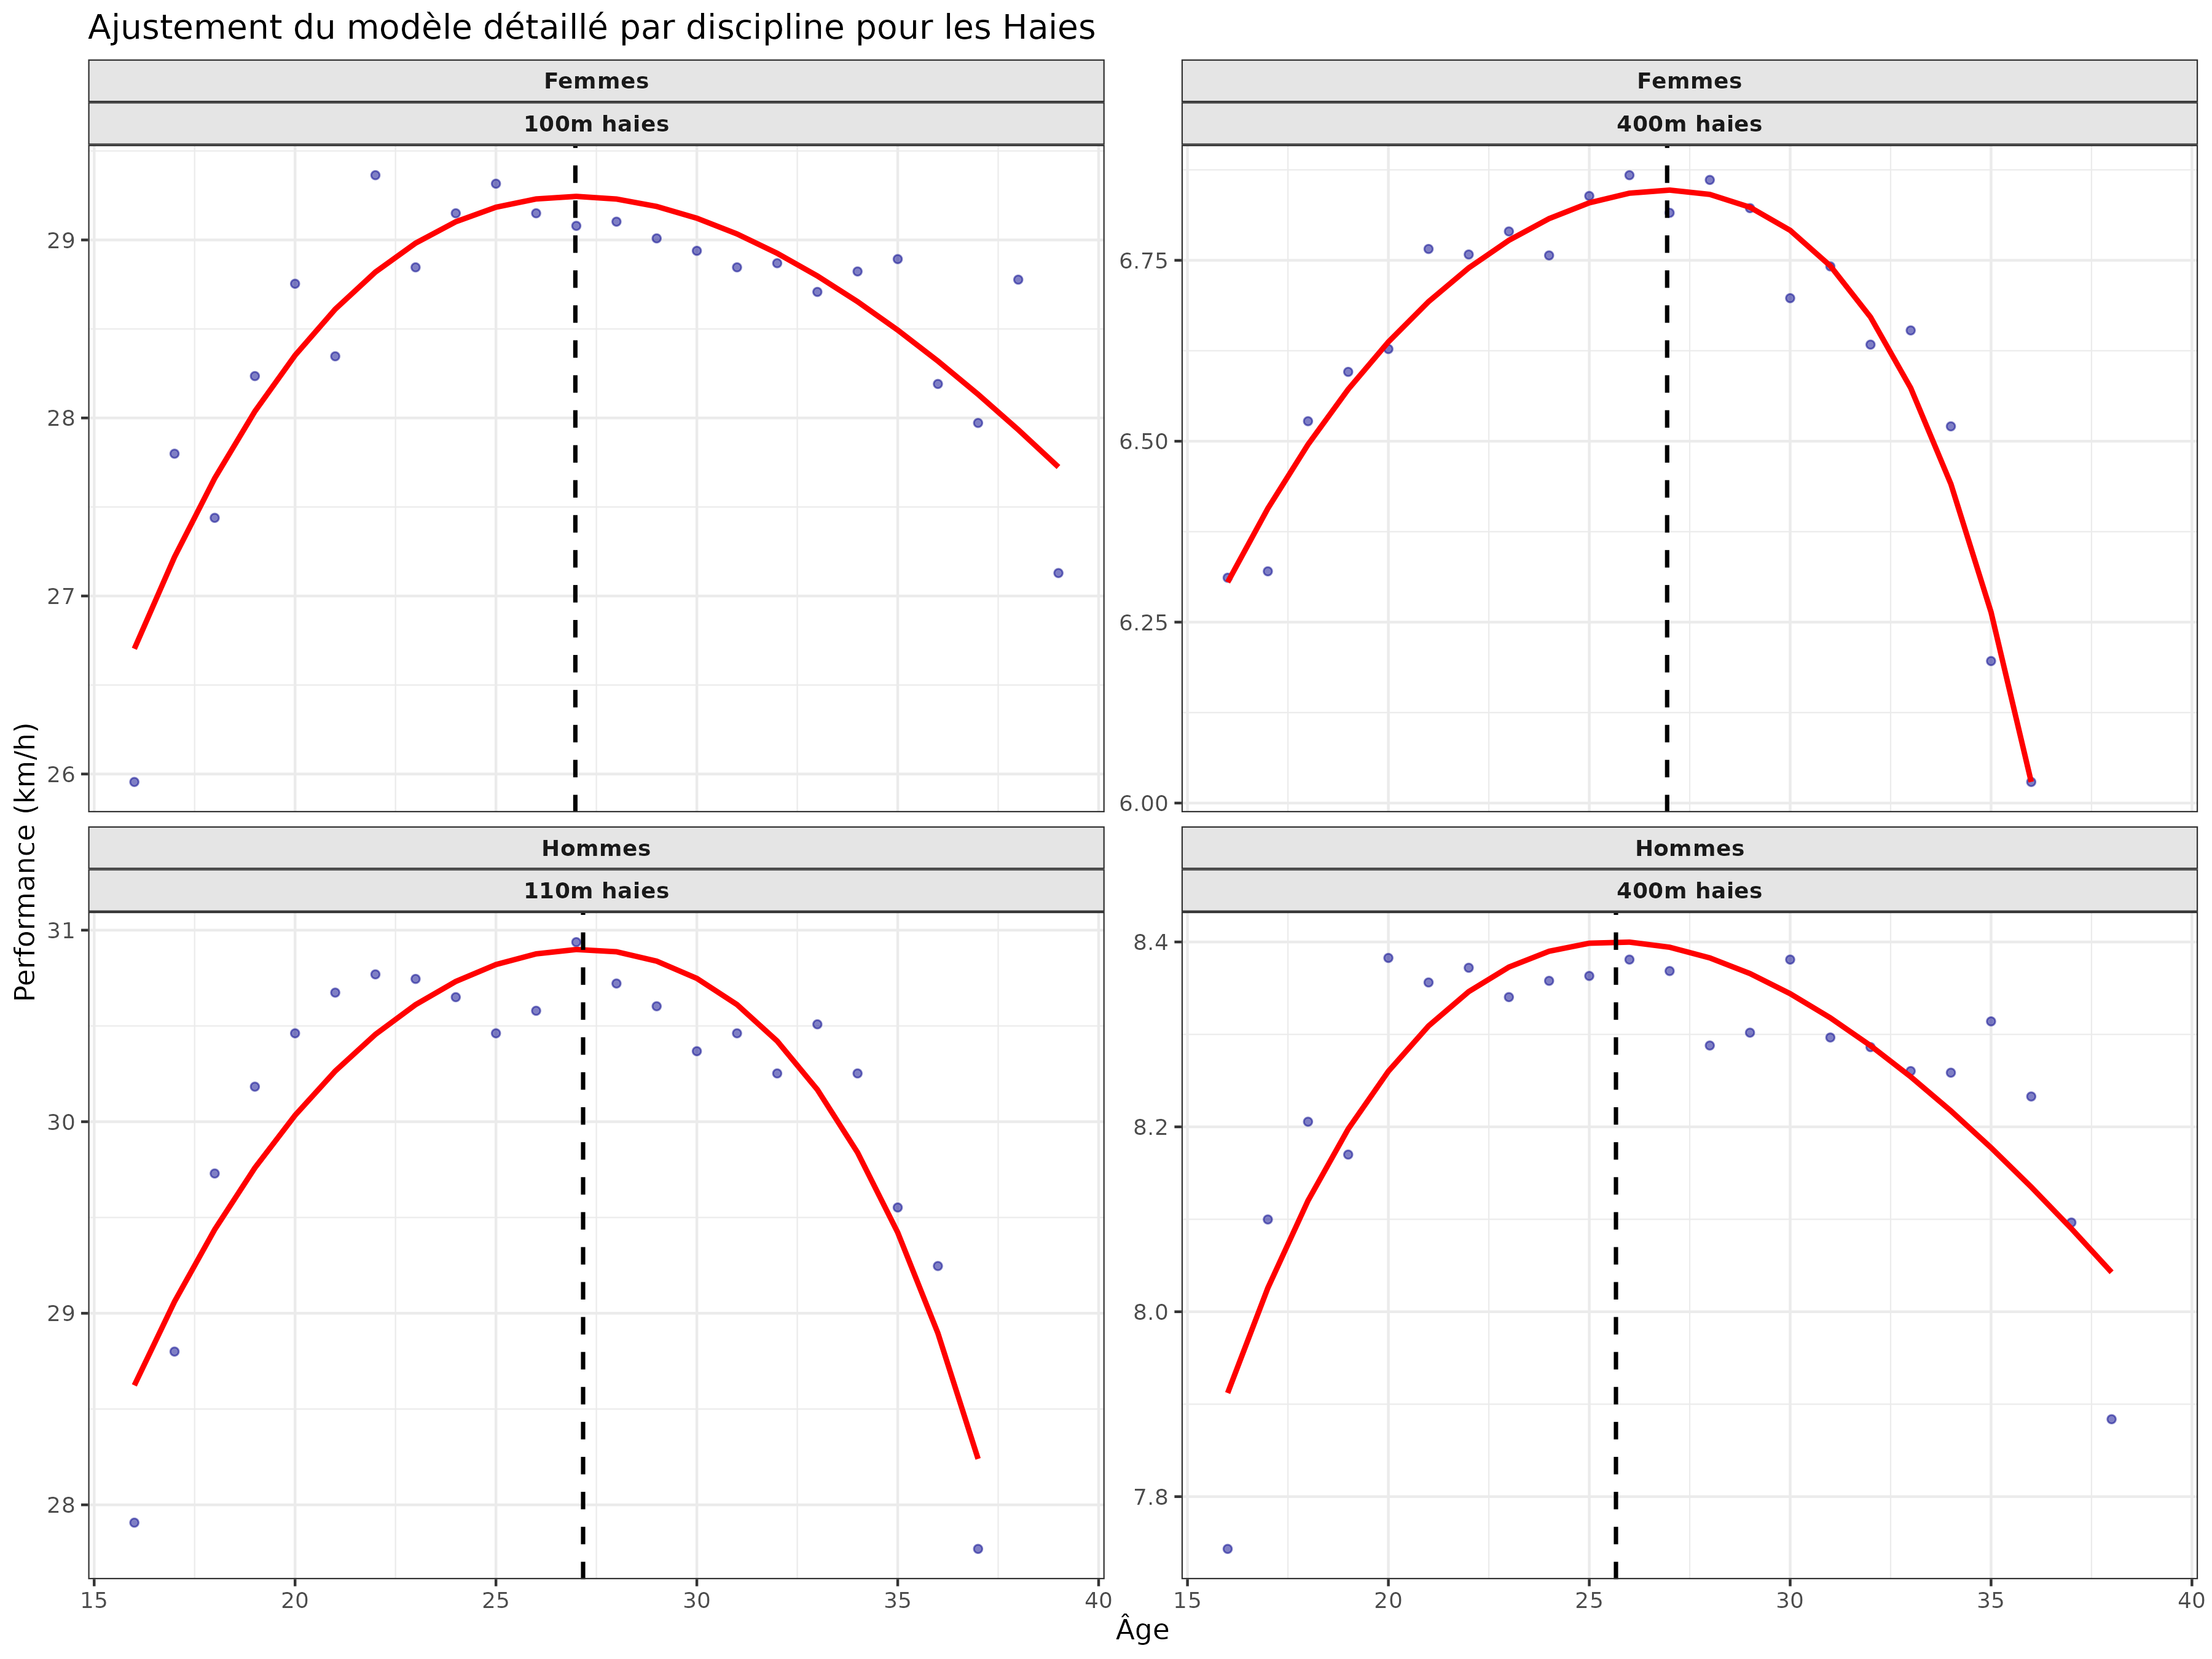
\includegraphics[width=0.8\linewidth,height=\textheight,keepaspectratio]{annexes/ajustement_haies.png}

}

\caption{Haies}

\end{figure}%

\begin{figure}[H]

{\centering 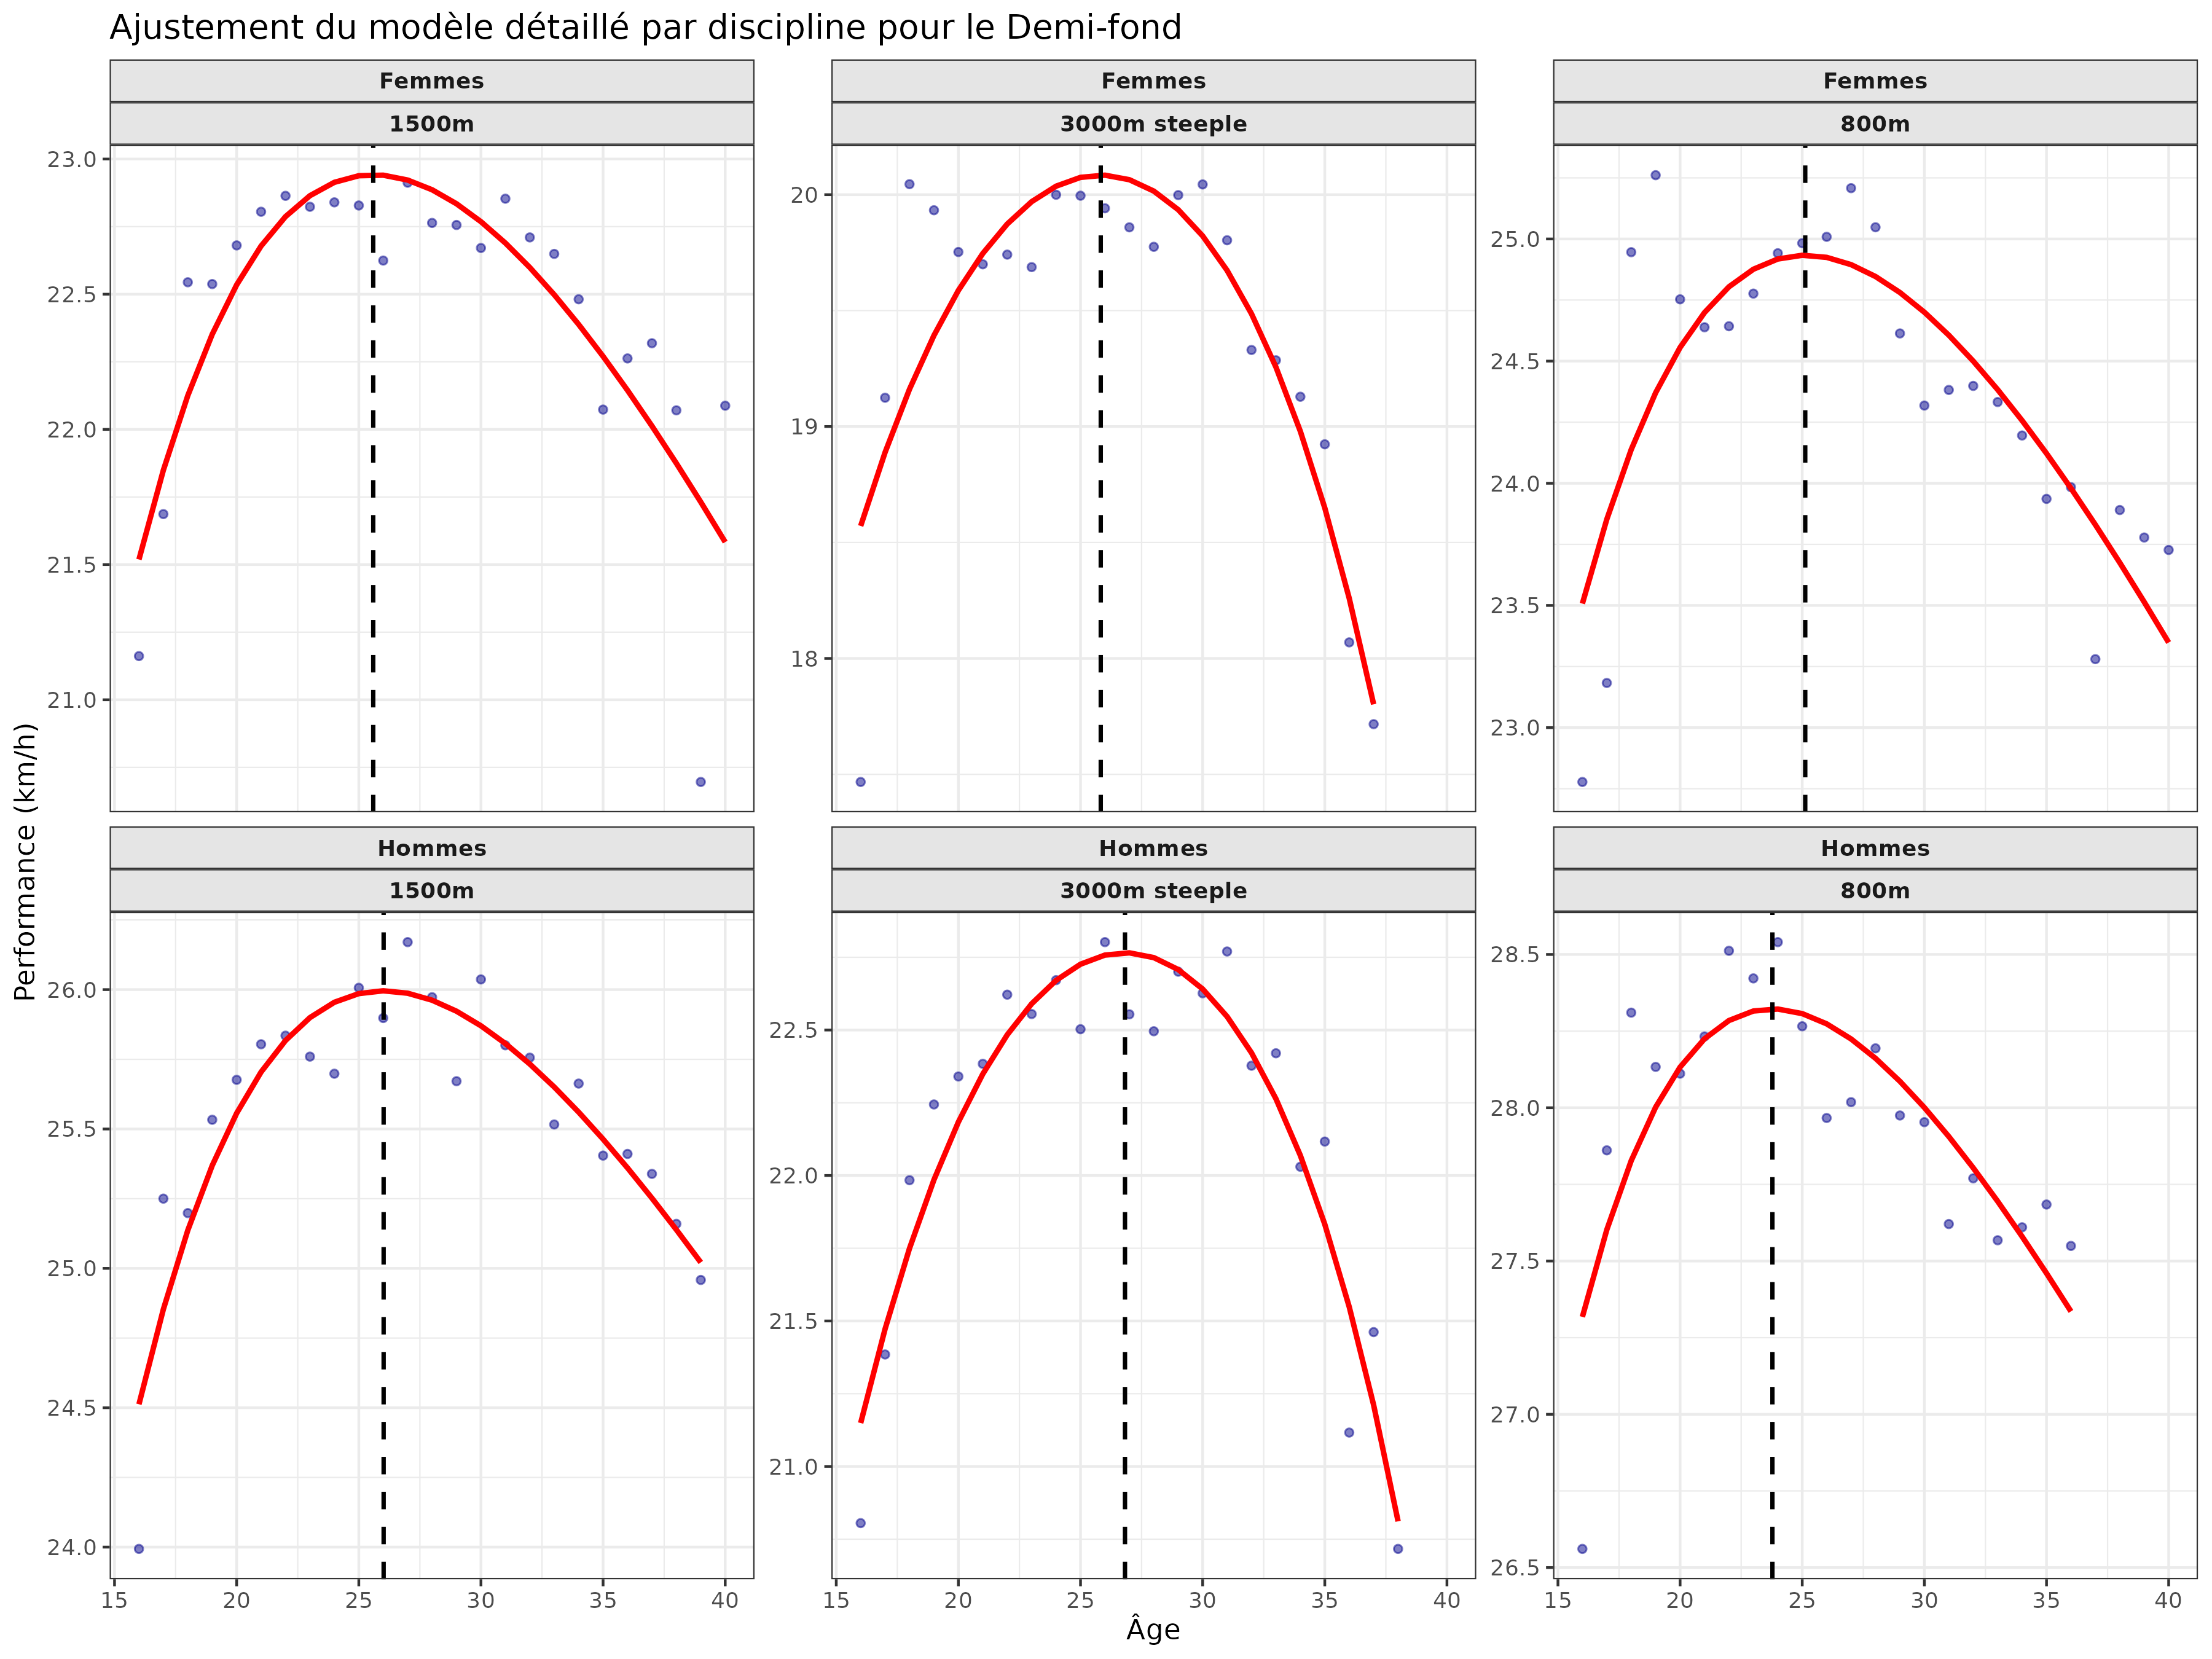
\includegraphics[width=0.8\linewidth,height=\textheight,keepaspectratio]{annexes/ajustement_demi_fond.png}

}

\caption{Demi-fond}

\end{figure}%

\begin{figure}[H]

{\centering 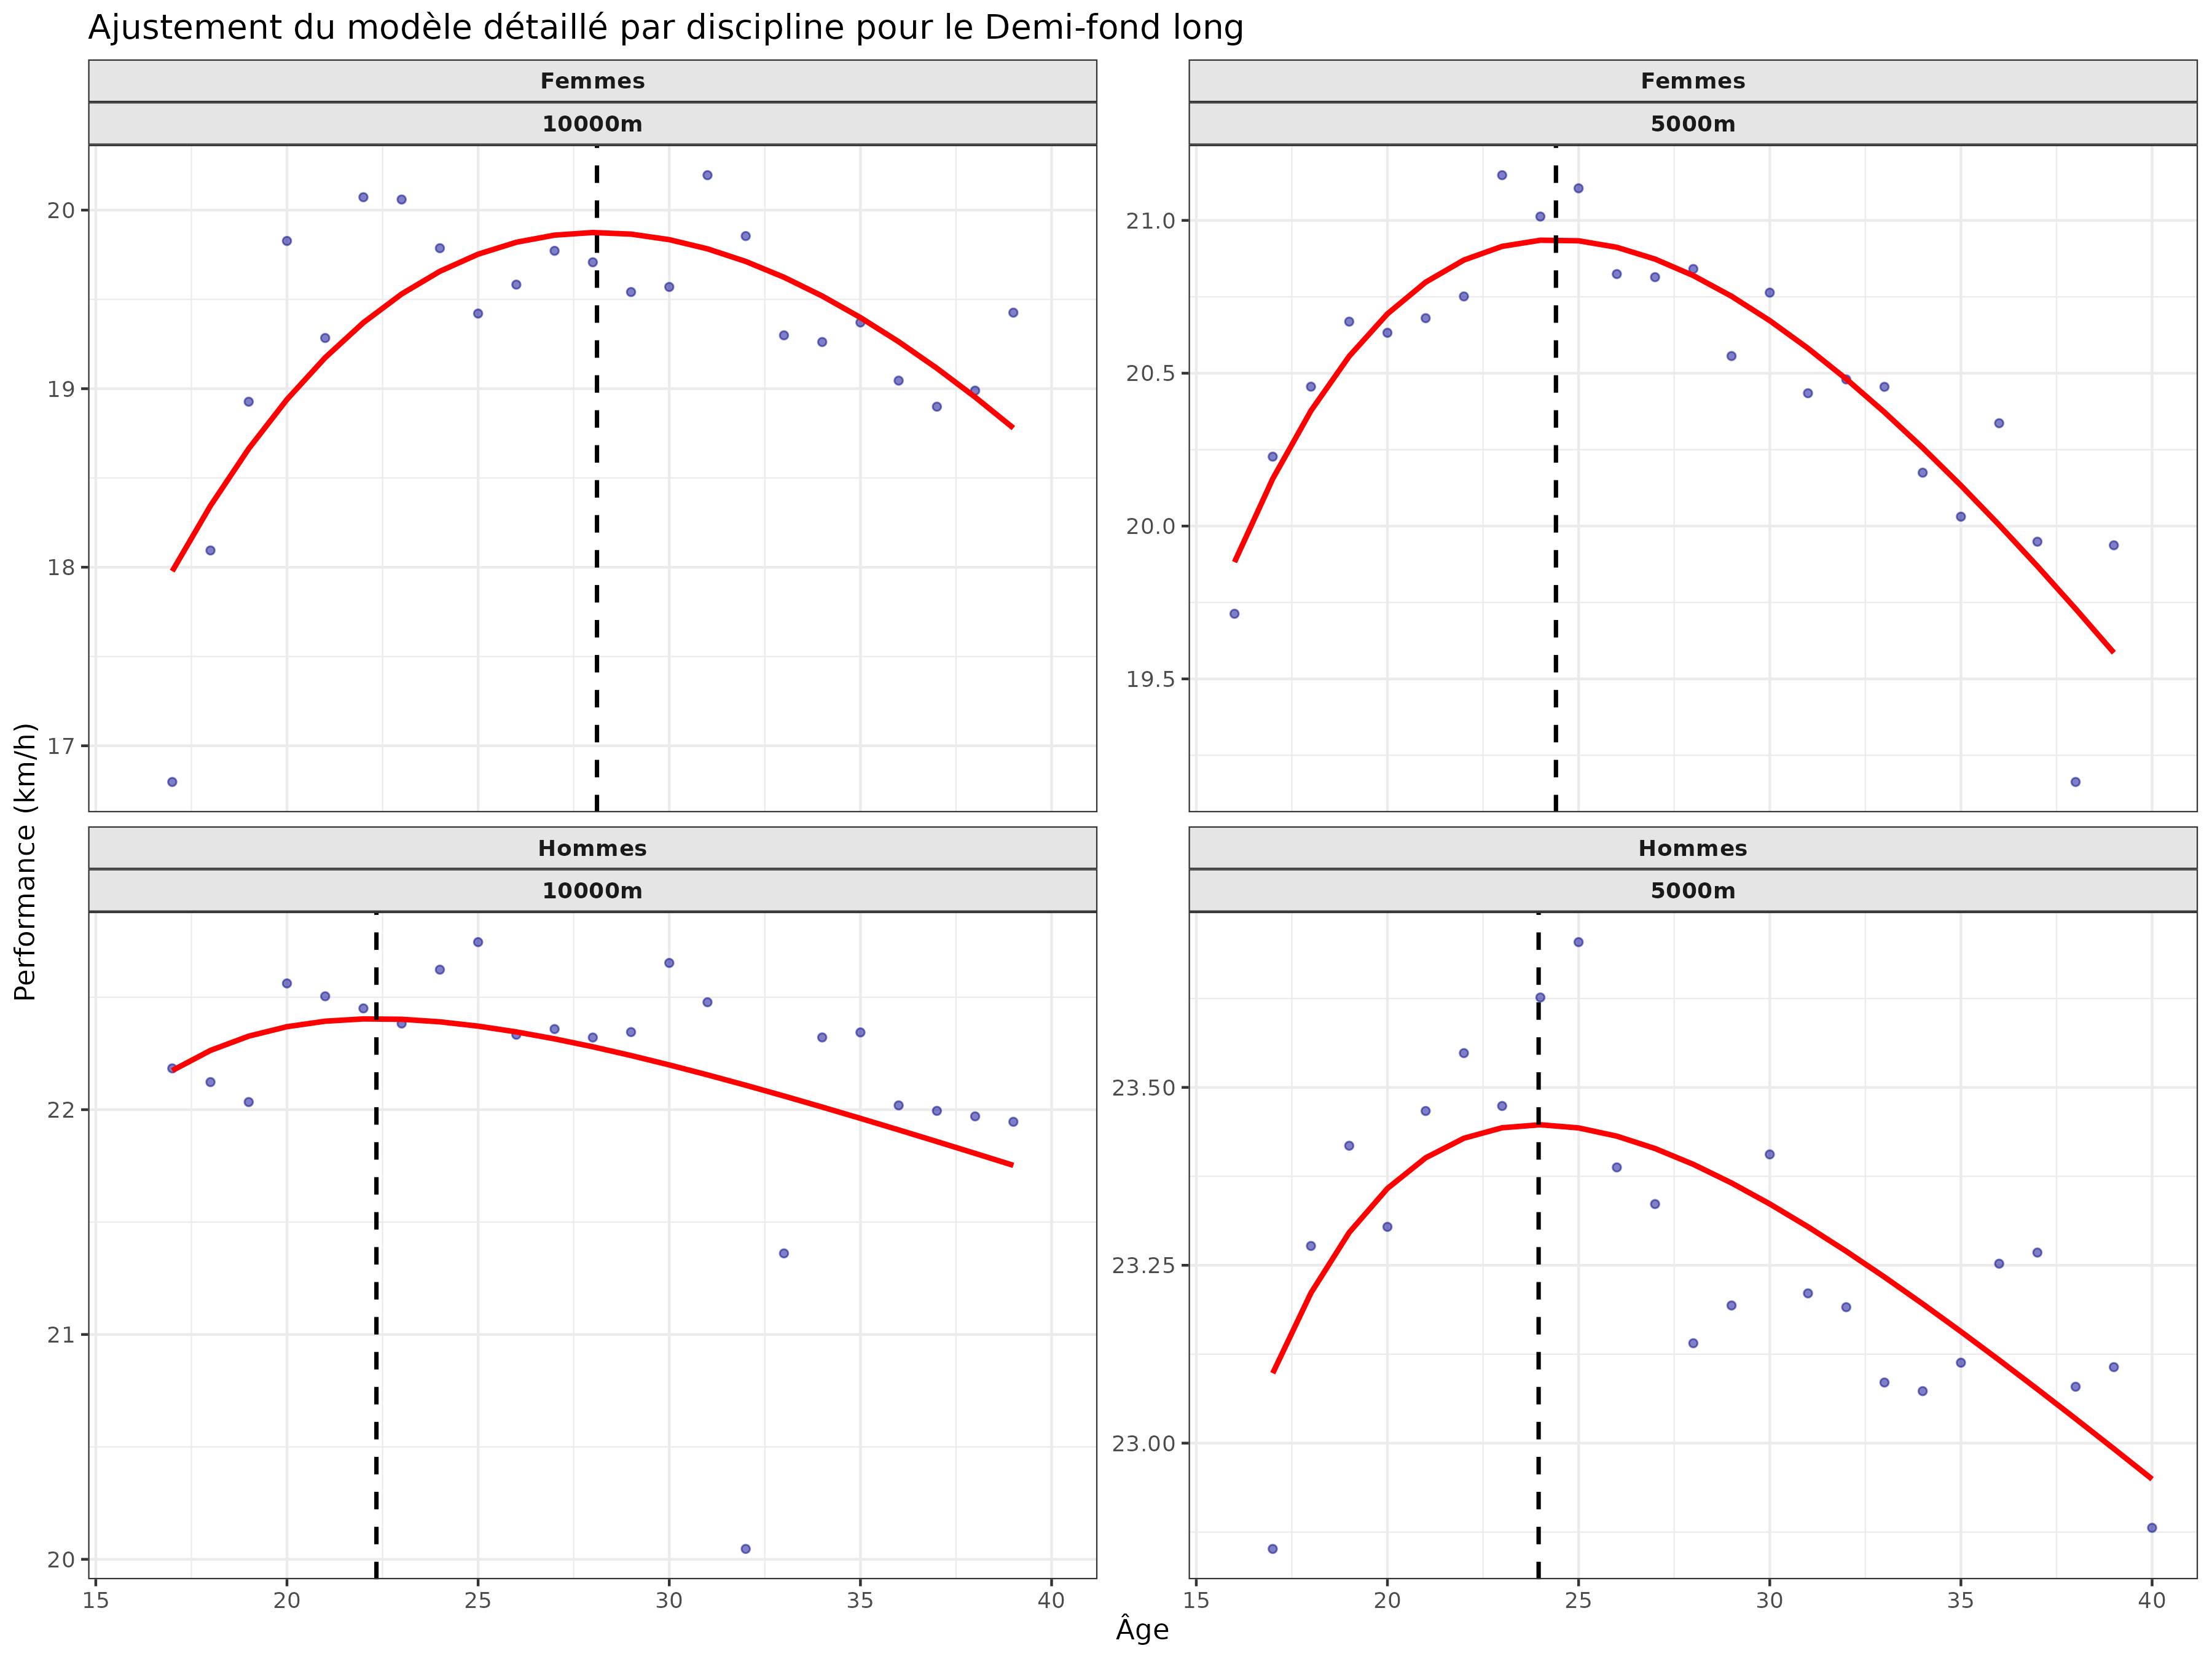
\includegraphics[width=0.8\linewidth,height=\textheight,keepaspectratio]{annexes/ajustement_5000_10000.png}

}

\caption{5000m - 10000m}

\end{figure}%

\begin{figure}[H]

{\centering 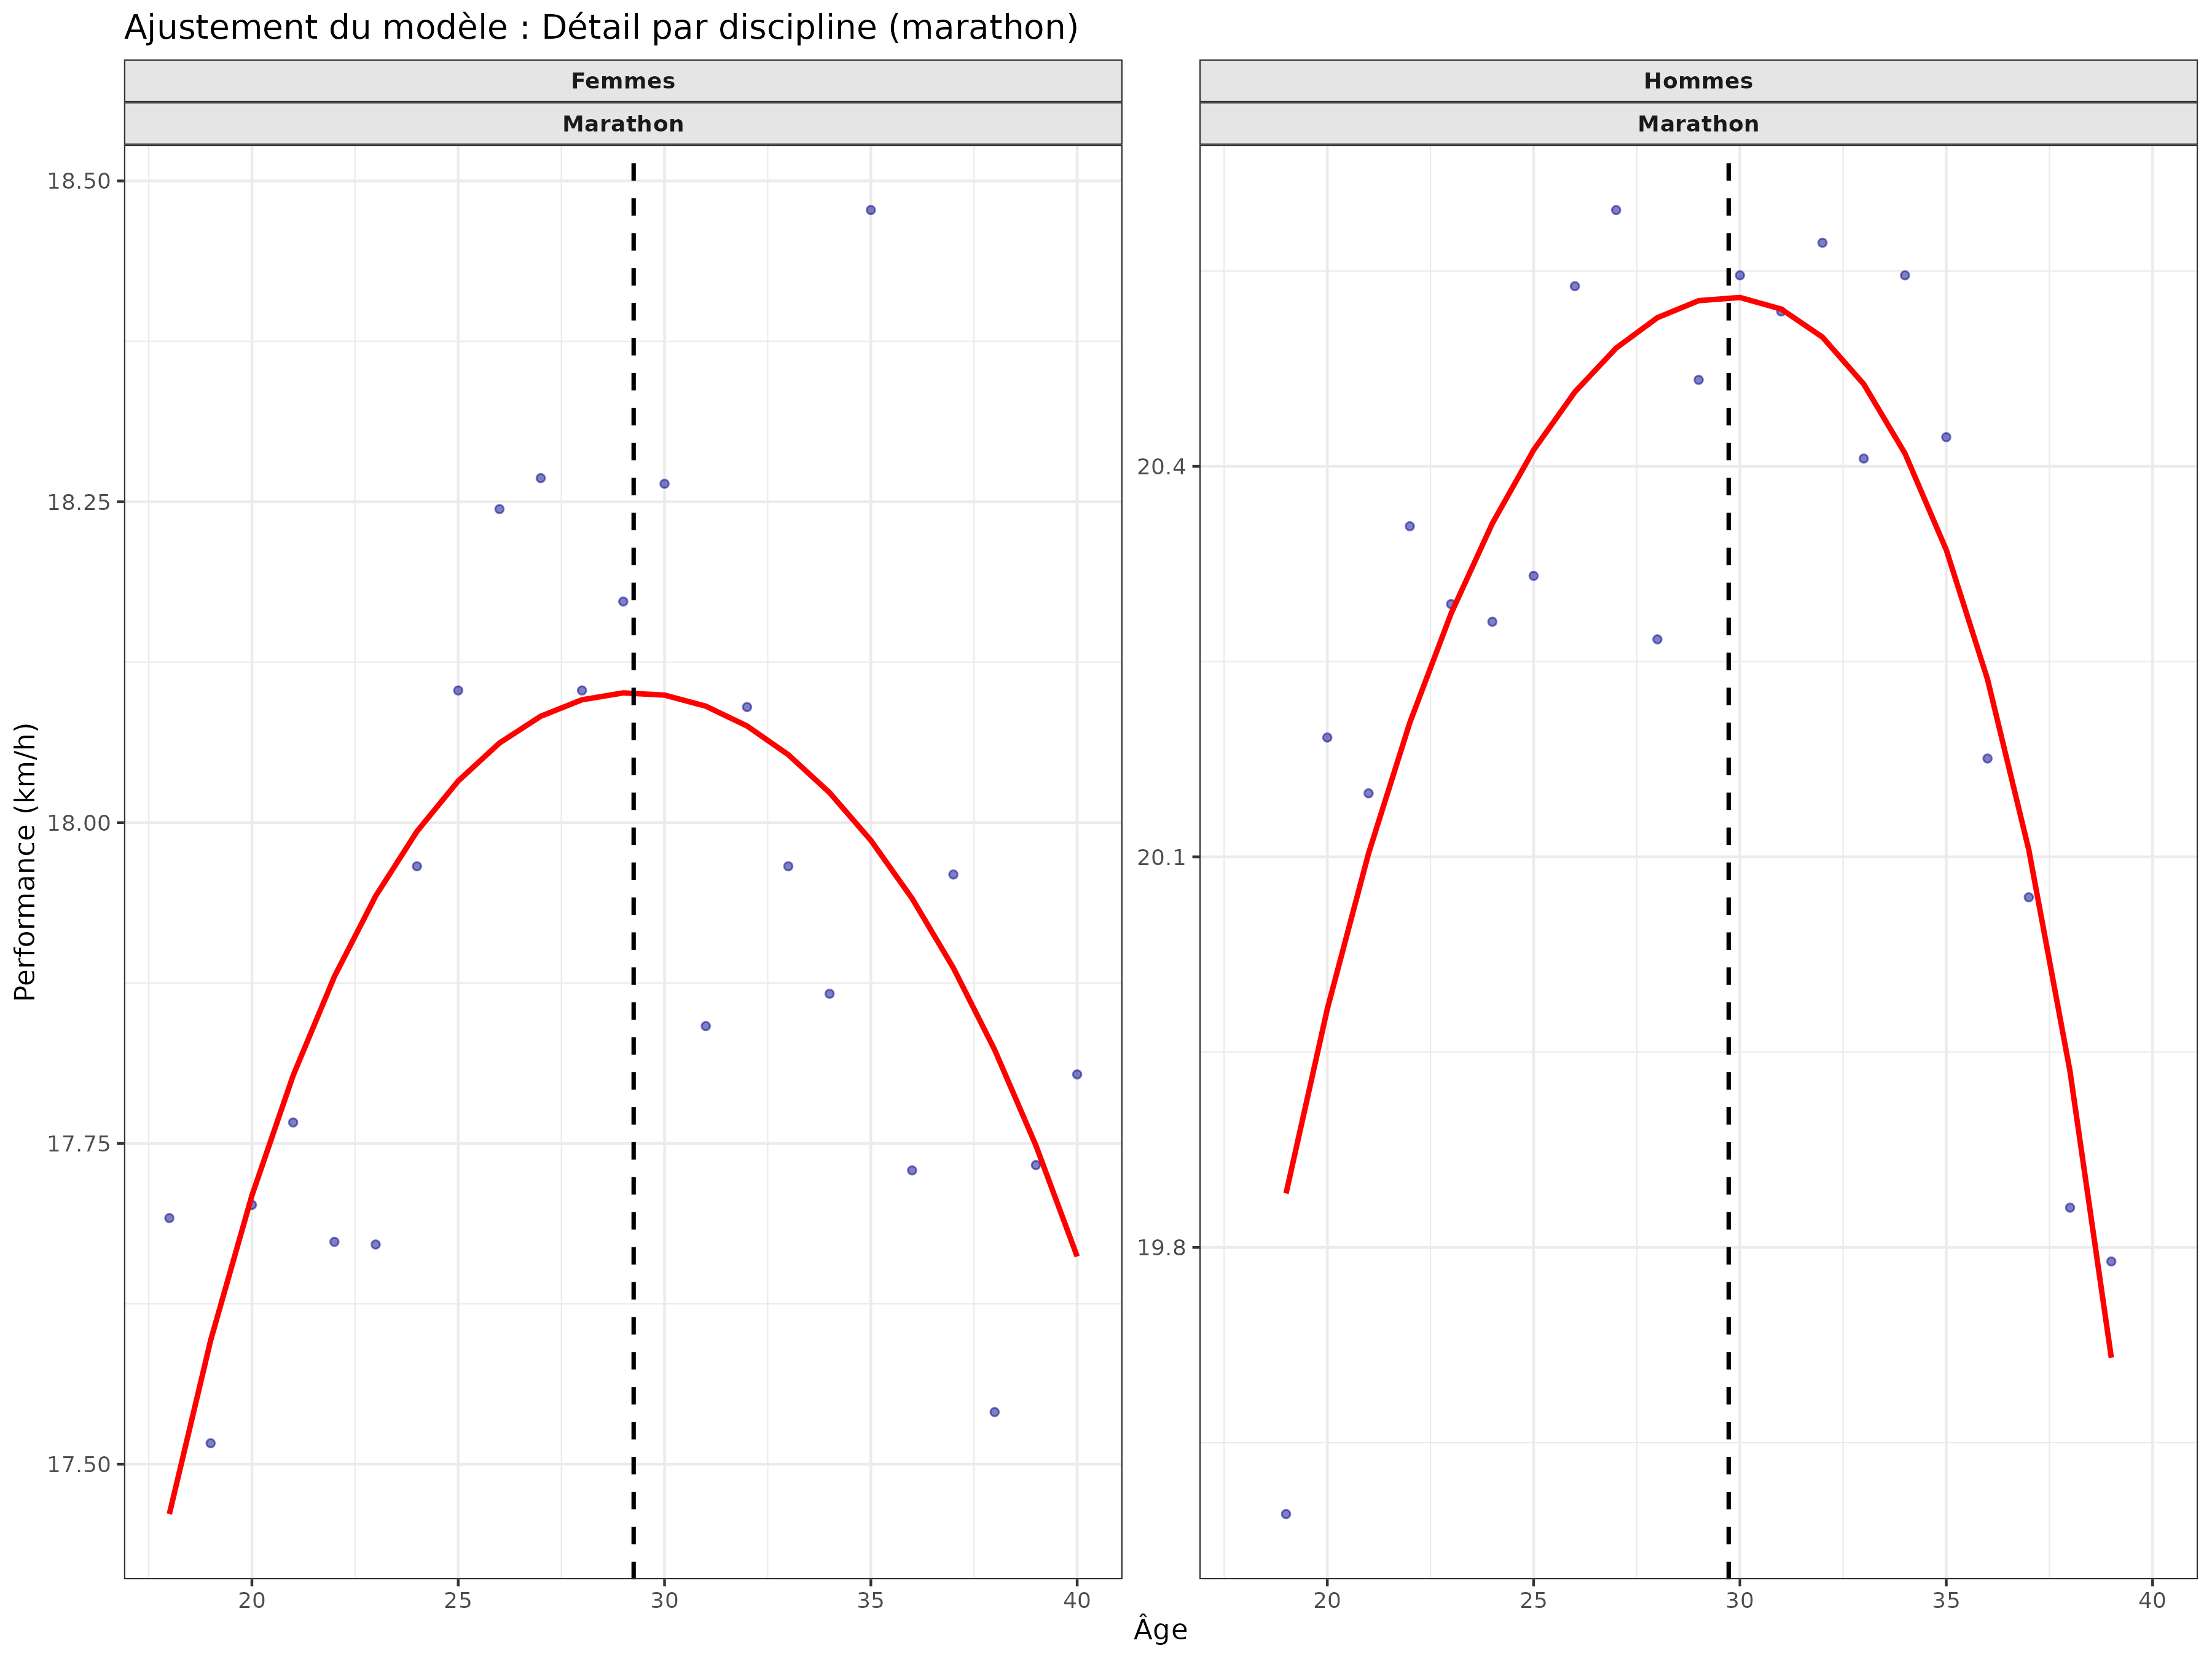
\includegraphics[width=0.8\linewidth,height=\textheight,keepaspectratio]{annexes/ajustement_marathon.png}

}

\caption{Marathon}

\end{figure}%

\begin{figure}[H]

{\centering 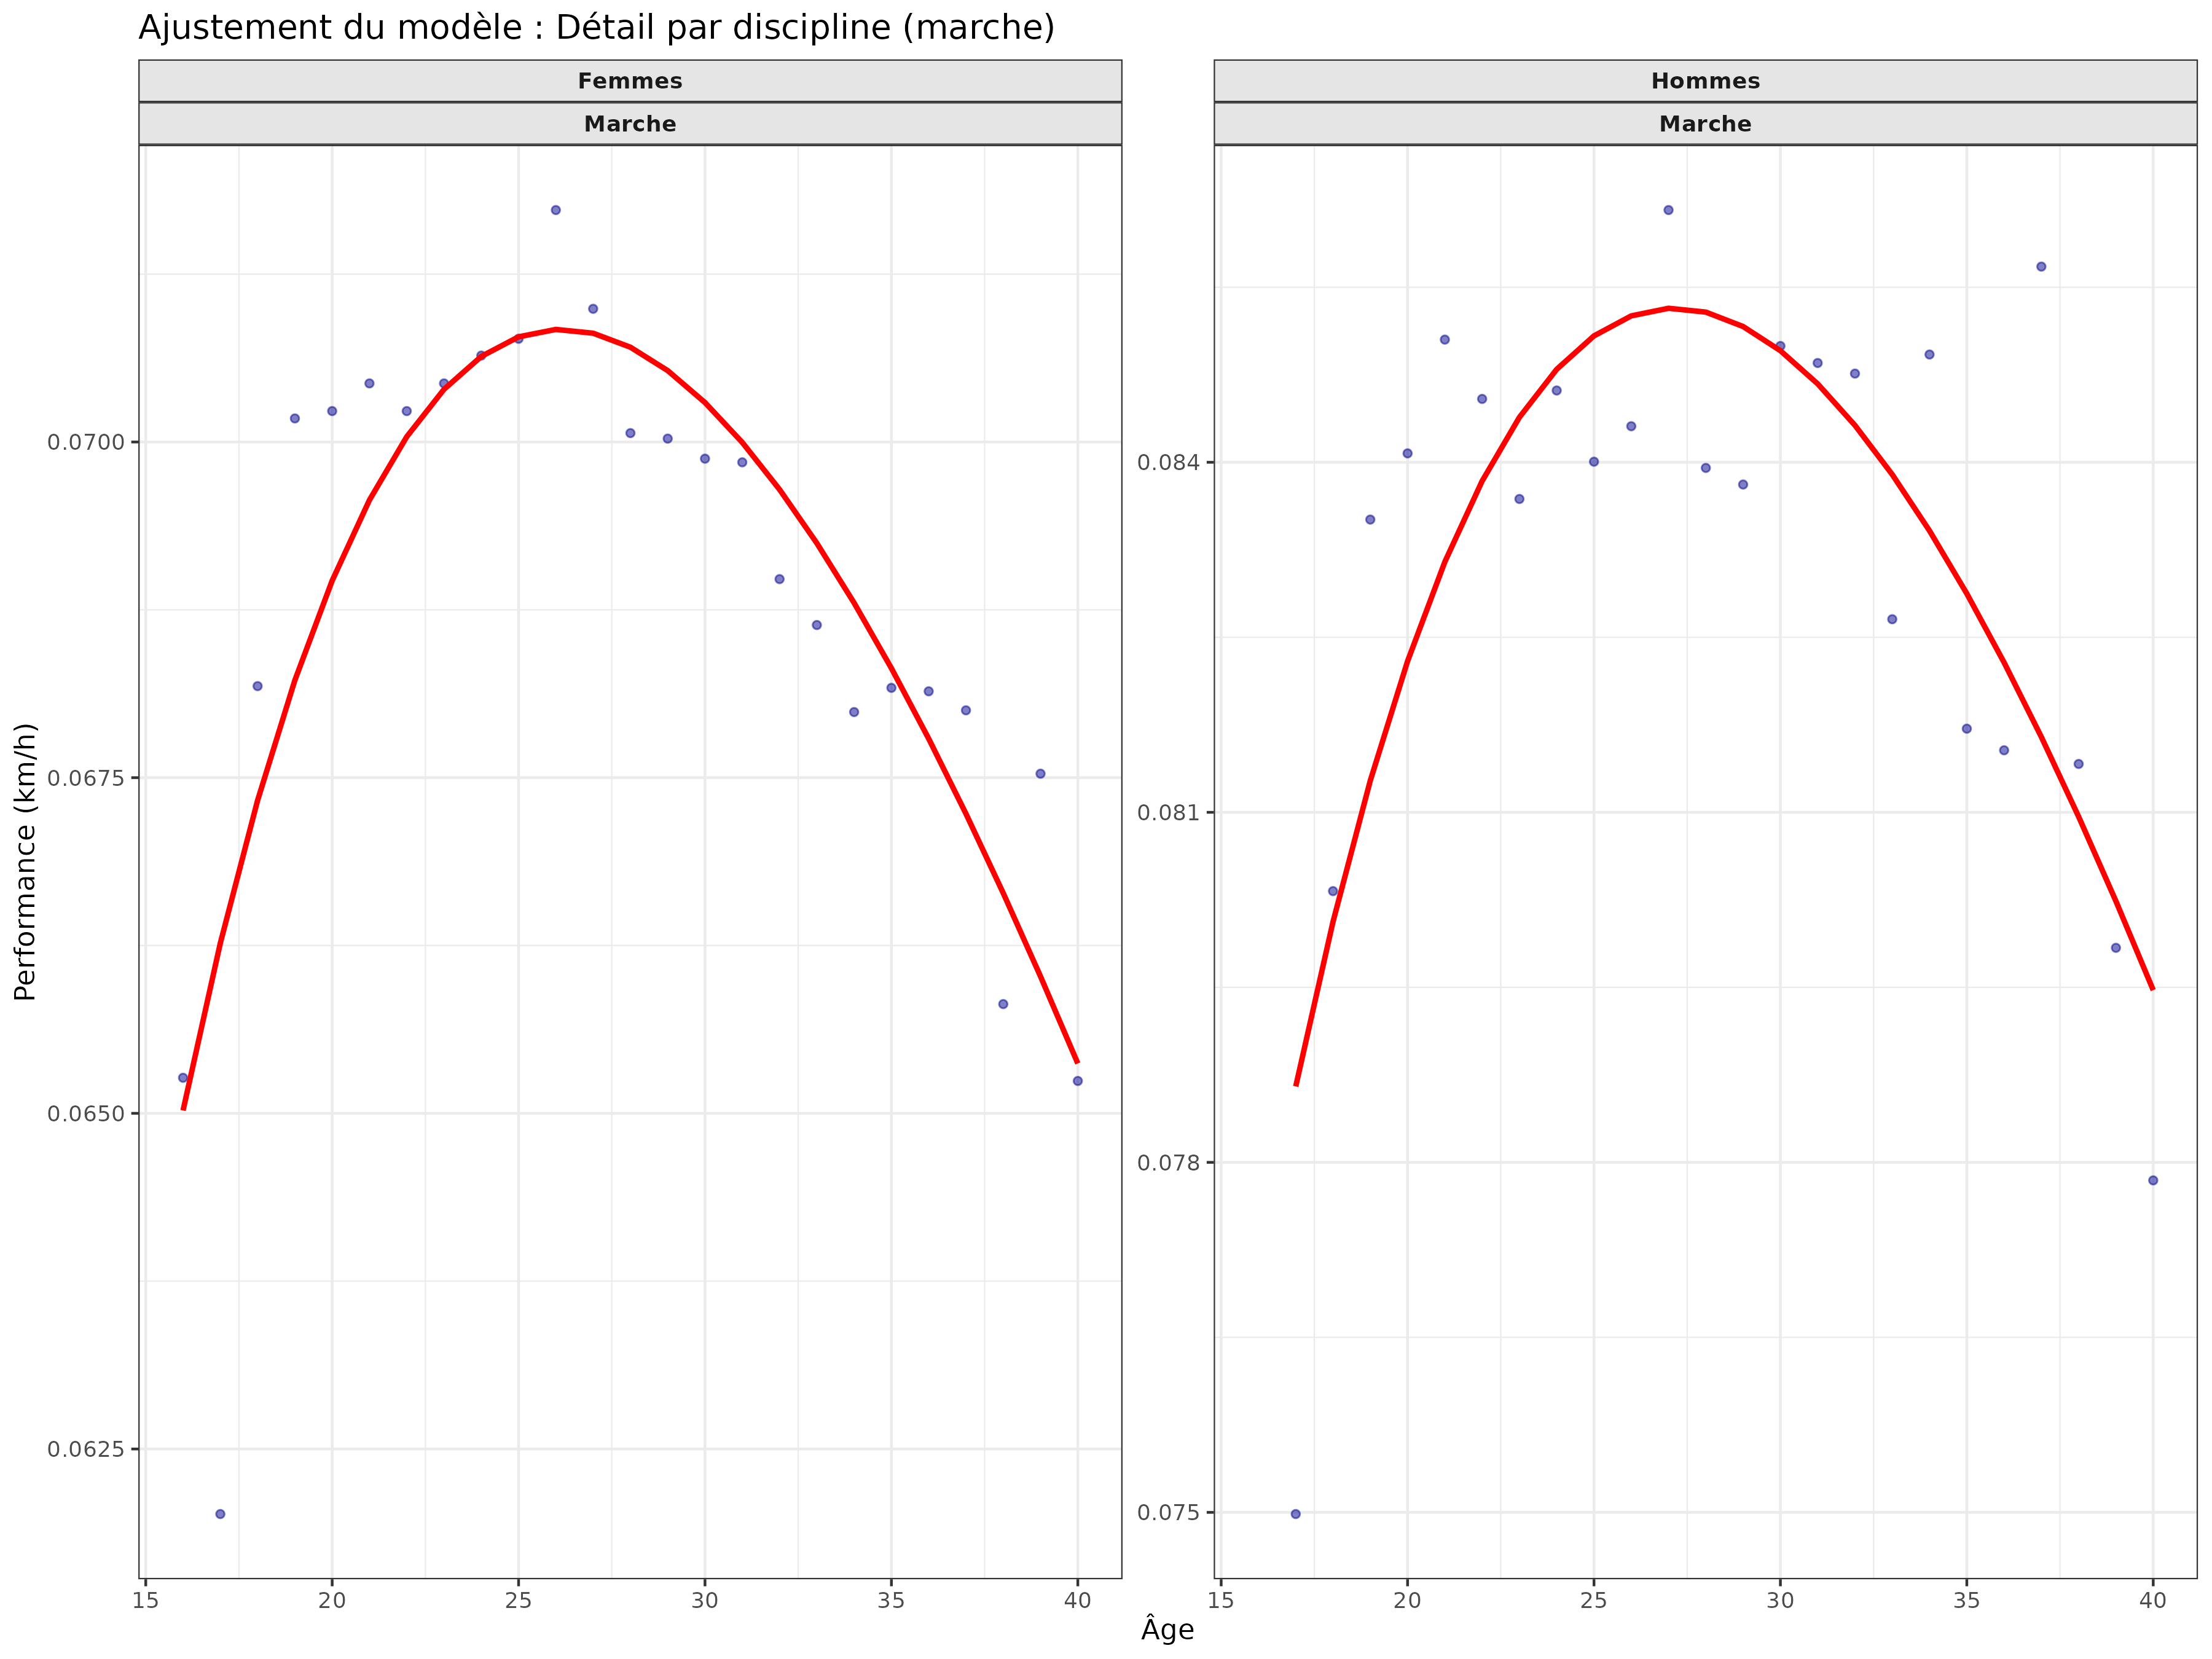
\includegraphics[width=0.8\linewidth,height=\textheight,keepaspectratio]{annexes/ajustement_marche.png}

}

\caption{Marche}

\end{figure}%

\begin{figure}[H]

{\centering 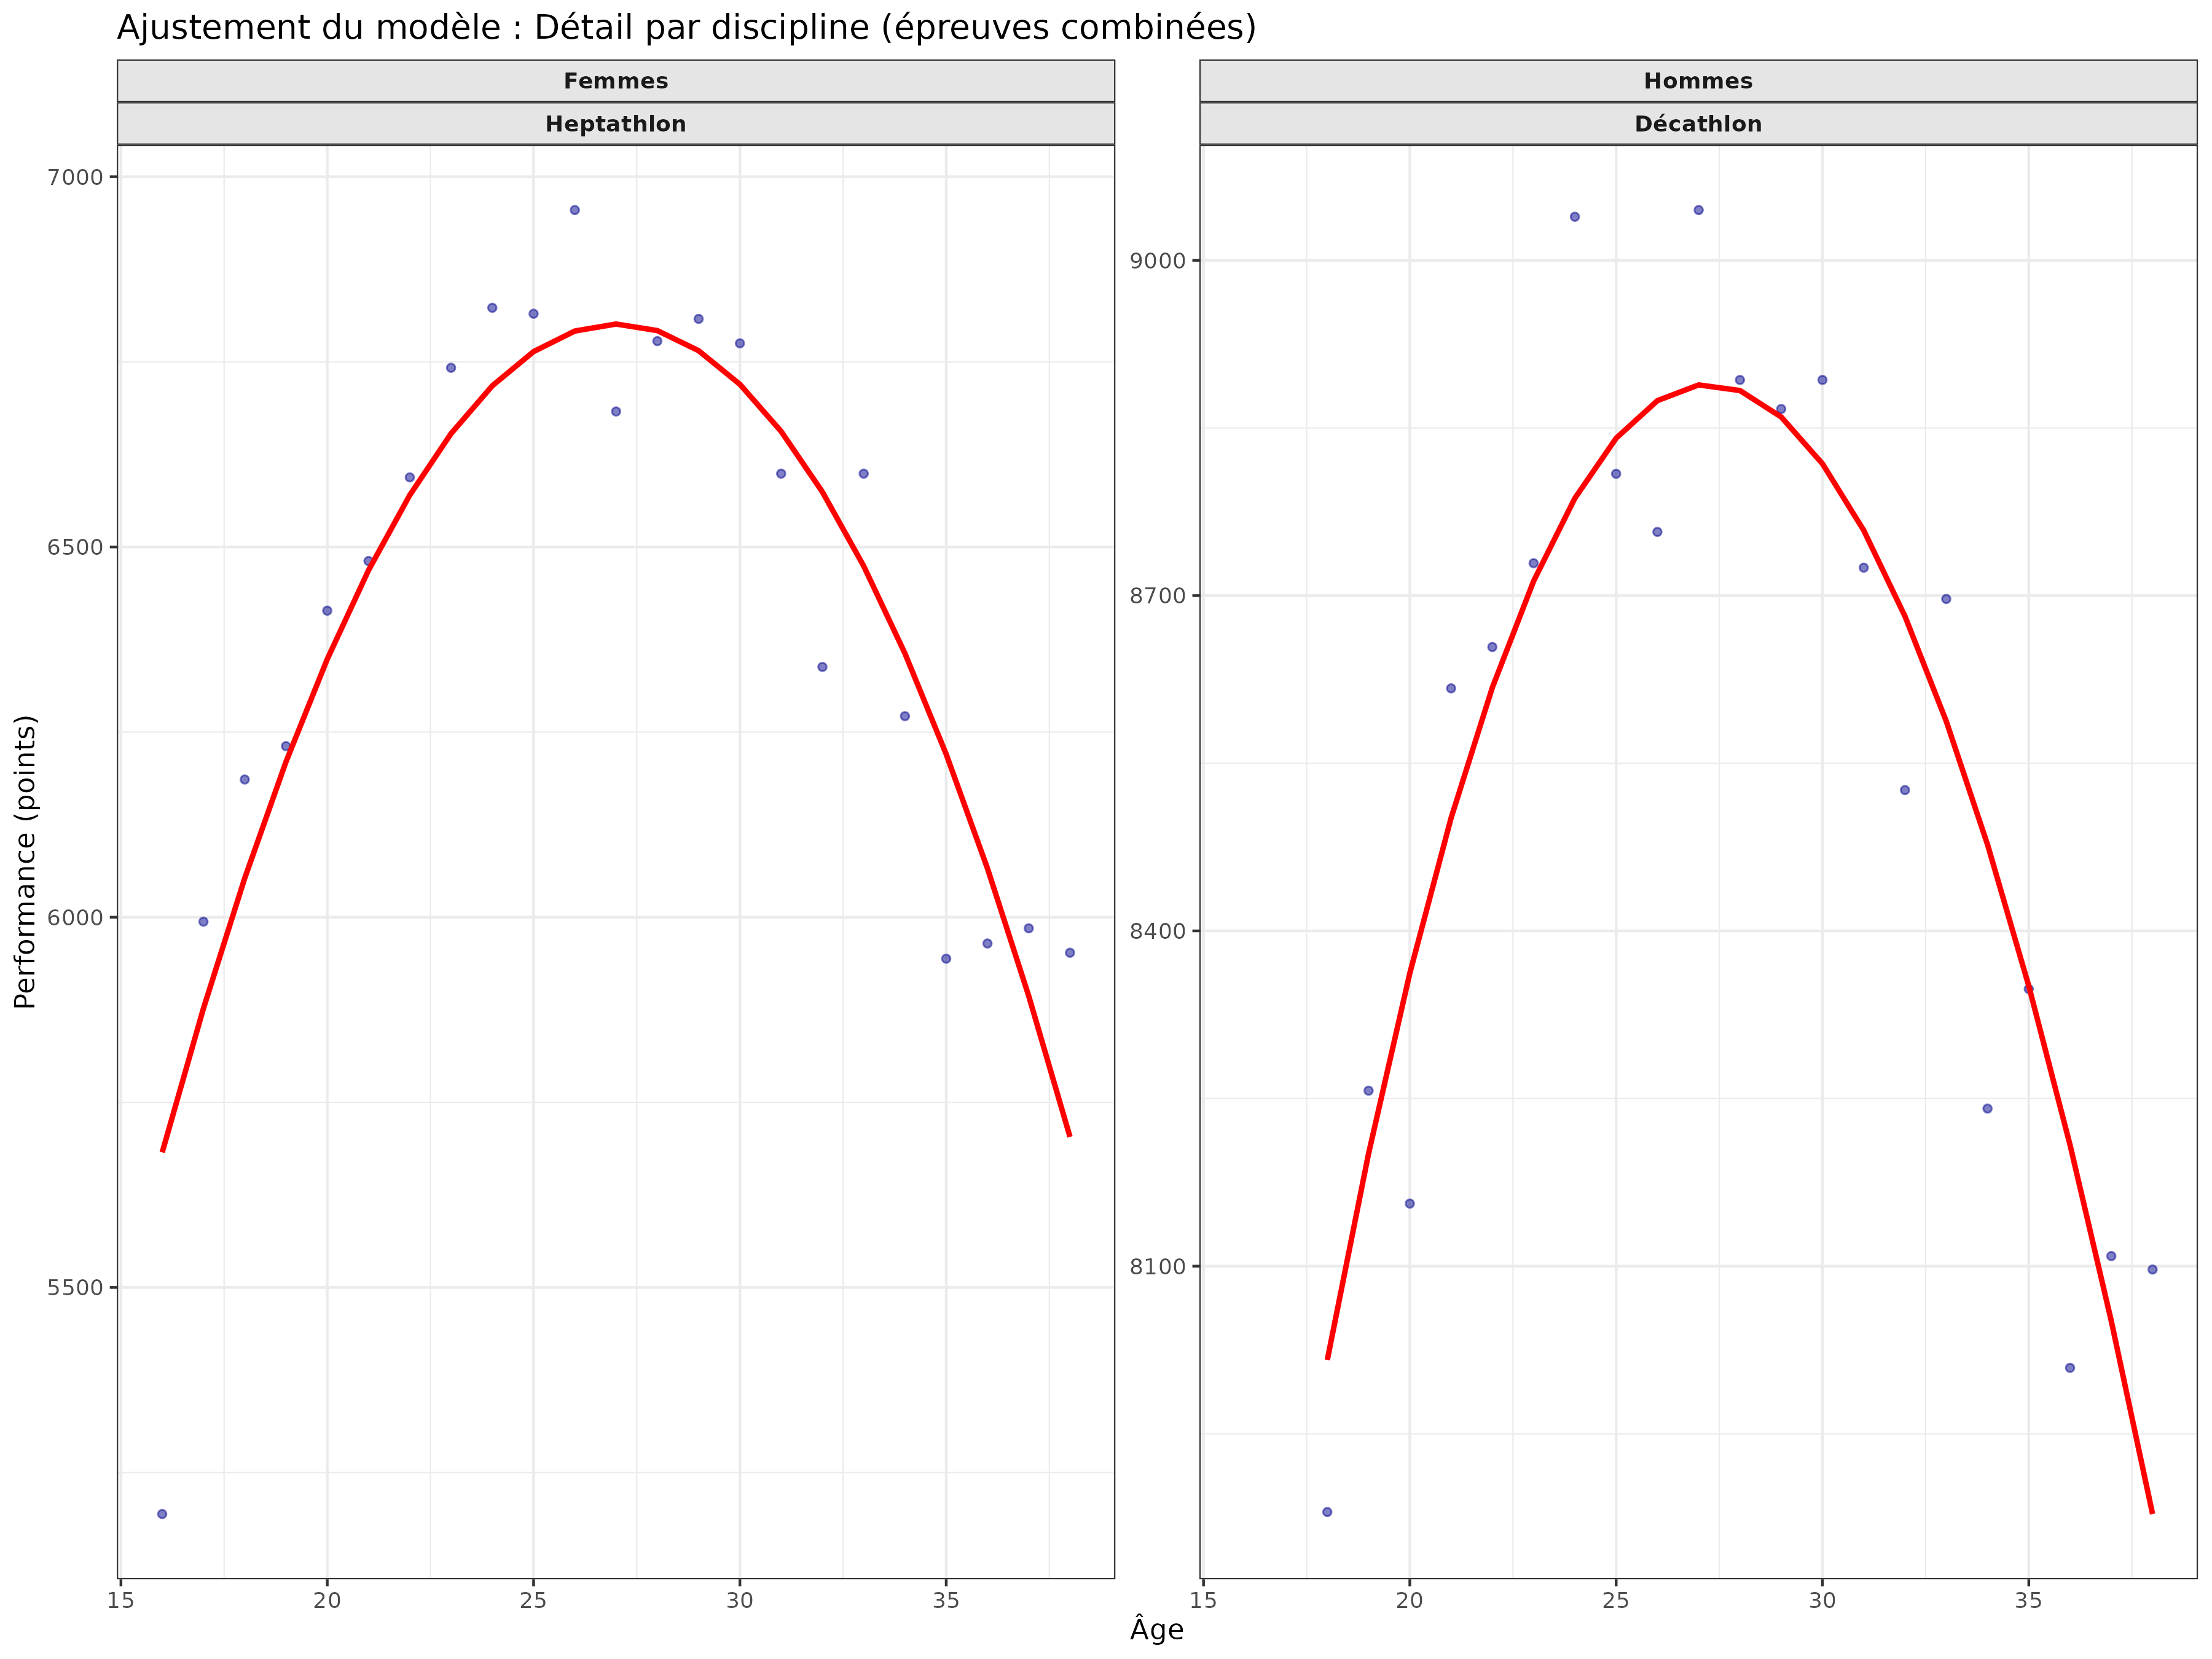
\includegraphics[width=0.8\linewidth,height=\textheight,keepaspectratio]{annexes/ajustement_epreuves_combinees.png}

}

\caption{Epreuves combinées}

\end{figure}%




\end{document}
